\documentclass[11pt]{report}



\usepackage[margin=1in]{geometry}  
\usepackage{graphicx}              
\usepackage{amsmath}               
\usepackage{amsfonts}              
\usepackage{amsthm}                
\usepackage{amssymb}
\usepackage{mathrsfs}
\usepackage{enumerate}
\usepackage{packages/algorithmic}
\usepackage{url}
\usepackage{packages/seqsplit}
\usepackage{packages/lettrine}
\usepackage{packages/type1cm}
\usepackage{packages/multirow}
\usepackage{hyperref}
\usepackage{tikz}
\usepackage{xcolor}
\usepackage[T1]{fontenc}
\usepackage{libertine}
\usepackage[libertine]{newtxmath}


\urlstyle{same}

%//////////////////////////////////////////////////////////////////////////////////////////////////

\definecolor{citecolor}{HTML}{009933}
% to make the refrences clickable, and...
\hypersetup{
	unicode = true,
    colorlinks = true,
    citecolor = citecolor,
    filecolor = blue,
    linkcolor = blue,
    urlcolor = blue,
    pdfstartview = {FitH},
}

%//////////////////////////////////////////////////////////////////////////////////////////////////
% theorem envirenments
\theoremstyle{plain}
\newtheorem{theorem}{Theorem}[chapter]
\newtheorem{lemma}[theorem]{Lemma}
\newtheorem{corollary}[theorem]{Corollary}
\newtheorem{proposition}[theorem]{Proposition}

\theoremstyle{definition}
\newtheorem{definition}[theorem]{Definition}
\newtheorem{conjecture}[theorem]{Conjecture}
\newtheorem{example}[theorem]{Example}
\newtheorem*{remark}{Remark}
\newtheorem*{note}{Note}

%//////////////////////////////////////////////////////////////////////////////////////////////////

\renewcommand{\algorithmicrequire}{\textbf{Input:}}
\renewcommand{\algorithmicensure}{\textbf{Output:}}
\algsetup{linenodelimiter=.}
\setlength{\parindent}{0pt}


\newcommand{\refchapter}[1]{Chapter \ref{#1}}
\newcommand{\refsection}[1]{Section \ref{#1}}
\newcommand{\refequation}[1]{Equation (\ref{#1})}
\newcommand{\reftheorem}[1]{Theorem \ref{#1}}
\newcommand{\reflemma}[1]{Lemma \ref{#1}}
\newcommand{\refcorollary}[1]{Corollary \ref{#1}}
\newcommand{\refproposition}[1]{Proposition \ref{#1}}
\newcommand{\refalgorithm}[1]{Algorithm \ref{#1}}
\newcommand{\refstep}[1]{Step \ref{#1}}


%//////////////////////////////////////////////////////////////////////////////////////////////////
% roman numerals
\newcommand{\romnum}[1]{\romannumeral #1}
\newcommand{\Romnum}[1]{\uppercase\expandafter{\romannumeral #1}}

%//////////////////////////////////////////////////////////////////////////////////////////////////


% characteristic of a field
\DeclareMathOperator{\fieldchar}{char}
% endomorphism ring
\DeclareMathOperator{\ringofend}{End}
% trace of a mtrix
\DeclareMathOperator{\trace}{tr}
% Galois group
\DeclareMathOperator{\gal}{Gal}
% order of an element
\DeclareMathOperator{\order}{ord}
% least common multiple
\DeclareMathOperator{\lcm}{lcm}
% divisor on a curve
\DeclareMathOperator{\divisor}{div}
% support of a divisor
\DeclareMathOperator{\supp}{supp}
% abs
\providecommand{\abs}[1]{\left\vert#1\right\vert}



%//////////////////////////////////////////////////////////////////////////////////////////////////
% The following allows algorithms to split over multiple pages
\makeatletter
\newcounter{algorithm}
\setcounter{algorithm}{0}
\renewcommand{\thealgorithm}{\thechapter.\arabic{algorithm}}
\def\algorithm{\@ifnextchar[{\@algorithma}{\@algorithmb}}
\def\@algorithma[#1]{%
  \refstepcounter{algorithm}
  \trivlist
  \leftmargin\z@
  \itemindent\z@
  \labelsep\z@
  \item[\parbox{\columnwidth}{%
    \hrule
    \hrule
    \noindent\strut\textbf{Algorithm \thealgorithm} #1
    \hrule
  }]\hfil\vskip0em%
}
\def\@algorithmb{\@algorithma[]}
\def\endalgorithm{\hfil\vskip-1em\hrule\endtrivlist}
\makeatother

% defined the end of proof symbol
\renewcommand{\qedsymbol}{$\square$}

%//////////////////////////////////////////////////////////////////////////////////////////////////
% overriding the proof env. for bold font 'Proof'
\makeatletter
\renewenvironment{proof}[1][\proofname]{\par
  \pushQED{\qed}%
  \normalfont \topsep6\p@\@plus6\p@\relax
  \trivlist
  \item[\hskip\labelsep
        \bfseries
    #1\@addpunct{.}]\ignorespaces
}{%
  \popQED\endtrivlist\@endpefalse
}
\makeatletter

%//////////////////////////////////////////////////////////////////////////////////////////////////

\newcommand{\keywords}[1]{\begin{description} \item[\textbf{Keywords.}] #1 \end{description}}

%//////////////////////////////////////////////////////////////////////////////////////////////////




\sloppy

\begin{document}
\pagenumbering{roman}
\thispagestyle{empty}
\vspace*{1.5in}
\begin{center}
\LARGE
\textbf{Point Counting On Genus 2 Curves} \\
\normalsize
\bigskip
%\isdefinedspinetitle{\spinetitle}
(Thesis format: Monograph)\\
\smallskip
\textbf{Javad \underline{Doliskani}}\\
\vspace*{1in}
Graduate Program in Computer Science\\
\vspace*{0.3in}
A thesis submitted in partial fulfillment\\
of the requirements for the degree of\\
Master of Science\\
\vspace*{0.3in}
The School of Graduate and Postdoctoral Studies\\
The University of Western Ontario\\
London, Ontario, Canada\\
\vfill
\copyright \hspace*{0.07in} J. N. Doliskani 2011  \\
\end{center}

%\addcontentsline{toc}{chapter}{Certificate of Examination}

\vspace*{0.5in}

\begin{center}

THE UNIVERSITY OF WESTERN ONTARIO \\
School of Graduate and Postdoctoral Studies \\

\bigskip

\textbf{CERTIFICATE OF EXAMINATION} \\

\vspace*{0.5in}

\begin{table}[h]
\centering
\begin{tabular}{p{8cm}|p{8cm}}
\parbox{3cm}{Supervisor \\ \vspace*{10mm}} & \parbox{3cm}{Examiners \\ \vspace*{10mm}} \\
\parbox{7cm}{\rule{7cm}{0.2mm} \\ \smallskip Dr. \'{E}ric Schost \\ \vspace*{0.2in}} 
& \parbox{7cm}{\rule{7cm}{0.2mm} \\ \smallskip Dr. Marc Moreno Maza \\ \vspace*{0.2in}} \\
& \parbox{7cm}{\rule{7cm}{0.2mm} \\ \smallskip Dr. J\'{an} Min\'{a}\v{c} \\ \vspace*{0.2in}} \\
& \parbox{7cm}{\rule{7cm}{0.2mm} \\ \smallskip Dr. Roberto Solis-Oba \\ \vspace*{0.2in}}
\end{tabular}
\end{table}


\vspace*{1cm}

The thesis by \\

\vspace*{0.2cm}

\textbf{Javad Nazari \underline{Doliskani}} \\

\vspace*{0.2cm}

entitled: \\

\vspace*{0.2cm}

\textbf{Point Counting On Genus 2 Curves} \\

\vspace*{0.2cm}

is accepted in partial fulfillment of the \\
requirements for the degree of \\
Master of Science \\

\vspace*{2cm}

\begin{table}[h]
\centering
\begin{tabular}{p{8cm}p{8cm}}
\parbox{7cm}{Date \rule{5cm}{0.2mm} \\ \smallskip} & \parbox{7cm}{\rule{7cm}{0.2mm} \\ \smallskip 
Chair of the Thesis Examination Board} 
\end{tabular}
\end{table}


\end{center}



%\addcontentsline{toc}{chapter}{Abstract}

\vspace*{2in}
\begin{center}
\large
\textbf{Abstract}
\normalsize
\end{center}

For cryptographic purposes, counting points on the jacobian variety of a given hyperelliptic curve 
is of great importance. There has been several approaches to obtain the cardinality of such a group, 
specially for hyperelliptic curves of genus 2. The best known algorithm for counting points on genus 
2 curves over prime fields of large characteristic is a variant of Schoof's genus 1 algorithm. 
Following a recent work of Gaudry and Schost, we show how to speed up the current state of the art 
genus 2 point counting algorithm by proposing various computational improvements to its basic 
arithmetical ingredients.

\keywords{Point counting, Hyperelliptic curves, Schoof's algorithm, Elliptic curves}

\tableofcontents

\pagenumbering{arabic}

\chapter{Introduction}
\label{chapter:intro}

\lettrine[findent=-0.5em, loversize=0.1]{A}{} one way function is, roughly speaking, a function that 
is easy to compute and hard to invert. The theory of one way functions forms the foundations of the 
modern cryptography \cite{Levin2003, Katz2008}. Given a certain finite cyclic group $G$, and a 
generator $g$ of $G$, the function
$$
\setlength\arraycolsep{2pt}
\begin{array}{llll}
\varphi: & \vmathbb{N}_{\le \abs{G}} & \longrightarrow & G \\
 & x & \longmapsto & g^x
\end{array}
$$
is expected to be a one way function. The problem of computing $\varphi^{-1}$ is called the 
\emph{discrete logarithm problem} (DLP) to the base $g$ in $G$. The security of many cryptographic 
schemes is based on DLP \cite{KoblitzMen2004, Odlyzko2000}. The group $G$ is suitable for this 
purpose if the DLP is hard in $G$, the elements of $G$ are easily and efficiently representable, 
computation in $G$ is fast, and the order of $G$ can be computed efficiently. As a general 
assumption, it is always assumed that $G$ has a non-smooth order, i.e. its order is a prime or a 
product of a large prime and some other very small factors; otherwise it is vulnerable to the 
Pohlig-Hellman attack \cite{Pohlig1978}. 

The traditional candidates for the group $G$ are multiplicative subgroups of finite fields. The 
arithmetic on finite fields is fast, but on the other hand, there are subexponential algorithms for 
computing discrete logarithm in these fields \cite{MenOorVan96}. Another candidate for the group 
$G$, proposed by Koblitz \cite{Koblitz1987} and Miller \cite{Miller1985} independently in 1985, is a 
cyclic subgroup of the group of points of an elliptic curve over a finite field. The advantage of 
systems based on such groups is that there is no known subexponential algorithm for DLP in these 
groups, for example the index-calculus algorithm does not apply to elliptic curves except to those 
of very special structures \cite{SilvermanSuz1998, Miller1985}. This leads to equally secure systems 
with smaller parameter sizes. The primary disadvantage of elliptic curve systems is that the 
addition of points is a relatively costly operation which is now reasonably fast due to the advances 
made in both theory and implementations, e.g. see \cite{Hankerson2004} and the references therein. 
Furthermore, Koblitz \cite{Koblitz1991, KoblitzDS1998} proposed a special family of curves allowing 
fast arithmetic. Computing the order of the group of a given elliptic curve is called point 
counting. There are polynomial time algorithms for counting points on elliptic curves, e.g. 
\cite{Schoof1985}. 

% references for Koblitz curves

As another candidate for group $G$ suitable for cryptosystems, Koblitz \cite{Koblitz1989} proposed 
the jacobian variety of a hyperelliptic curve over a finite field, which is indeed a generalization 
of the elliptic case. This leads to even smaller field sizes, and larger number of choices. Also, 
the elements of the jacobian can be represented using pairs of finite degree polynomials called the 
Mumford representation. According to Riemman-Roch theorem, there is a unique integer attached to 
every curve, called the genus of the curve. For example, a curve is elliptic if and only if it is 
genus one with at least one rational point. The main drawback of the hyperelliptic curve systems is 
that the addition on the jacobian is generally slower than the group operation on elliptic curves, 
and the higher the genus goes the slower would be the arithmetic. Moreover, for large enough genera, 
there is a version of index-calculus method for computing the discrete logarithm in the jacobian 
\cite{Adleman1994, Enge2002, Muller1999, GaudryDL2000}. 

In terms of efficiency, genus 2 curves provide the closest hyperelliptic alternative for elliptic 
curve cryptosystems \cite{Pelzl2003, Gaudry2007, TLange2005}. Furthermore, for an equally secure 
system, and the same parameter lengths, the base field for the genus 2 curve is almost twice 
smaller. To find secure hyperelliptic curves, there are two main approaches:
\begin{description}
\item[Point counting] In which one tries several random curves over a given finite field until a 
good one is found, and then computes the cardinality of the jacobian.
\item[CM method] In which, instead of trying random curves, one starts with the endomorphism ring 
and vary the base field until a curve with a good jacobian order is found, e.g. \cite[ch. 
18]{Cohen2006}, and \cite{Weng2003}. 
\end{description}
There are other methods, e.g. \cite{Sutherland2009}, that work under special conditions. There are 
also known special families of curves with good jacobian order, e.g. \cite{Koblitz1988a}. The 
complex multiplication method is efficient, but curves found by this method have more special 
structures, and it is not generally known if they are stronger or weaker than general curves. In 
this thesis, we investigate point counting on genus 2 curves.

Various approaches have been proposed for point counting on hyperelliptic curves, from which we can 
name (\textbf{\romnum{1}}) Schoof's algorithm which is the generalization of the Schoof's algorithm 
for elliptic curves, and it is polynomial time. (\textbf{\romnum{2}}) Kedlaya's algorithm 
\cite{Kedlaya2001} which is exponential time in general, but efficient in small characteristics. 
(\textbf{\romnum{3}}) Satoh's algorithm \cite{Satoh2000} which is polynomial time in small 
characteristic, but exponential in general. The best of the above approaches, for large 
characteristics, is the Schoof's algorithm. The generalization is essentially due to Pila 
\cite{Pila1990}. The Schoof's algorithm for hyperelliptic curves of genus 2 was then presented in 
Gaudry and Harley \cite{GauHar2000}, and Gaudry and Schost \cite{GauSch2004, GASC2010}. In 
particular, the following is the timeline for point counting on genus $2$ curves.
\begin{itemize}
\item Gaudry and Harley (2000): 126 bit Jacobian
\item Gaudry and Schost (2004): 164 bit, secure Jacobian
\item Sutherland (2007): 188 bit, secure Jacobian (works for special curves)
\item Gaudry and Schost (2008): 256 bit, secure Jacobian
\item Gaudry and Schost (present): 256 bit, doubly-secure Jacobian
\end{itemize}
In this thesis, we show how to improve the work of Gaudry and Schost by improving the arithmetical 
ingredients of their algorithm both theoretically and in terms of implementation. According to their 
most recent work, their algorithm makes extensive use of square (or higher) root computing, modular 
polynomial composition, and power projection. Both modular polynomial composition, and power 
projection are based on  matrix multiplication. For example, to have a fast modular polynomial 
composition, the natural choice is the algorithm of Brent and Kung \cite{BreKun1978}, which is still 
practically the best. So, we have  proposed and implemented an algorithm for fast multiplication of 
matrices with integer entries of arbitrary length. This small parallel low level library, with high 
level interfaces, is embedded into the NTL library \cite{NTL2009}. Consequently, the new modular 
composition, and power projection implementations have been embedded into NTL. For the square root 
computation, we have proposed a new algorithm, implemented it, and integrated it into NTL. This 
algorithm uses polynomial composition for computing a trace-like map that reduces the problem to the 
same problem over the prime field.

In this thesis, rather than an abstract general description of materials, specially the theory of 
elliptic and hyperelliptic curves, we have tried to conduct a concrete and intuitive approach. We 
have made an effort to make this document as self contained as possible with respect to the needed 
materials by giving clean proofs, unless the proofs are too long or there is no point in quoting 
other's proofs. The reader is assumed to have a basic knowledge of algebra, and polynomial 
arithmetic. We shall denote the asymptotic complexity bounds of polynomial multiplication, and 
modular polynomial composition by $O(M(n))$, and $O(C(n))$ respectively. The best known $M(n)$ is 
$n\log n\log\log n$ achieved by using Fast Fourier Transform (FFT) \cite{Schonhage1971}, and the 
best know $C(n)$ is $n^{1.69}$. See \refsection{section:MMapll} for more details on $C(n)$.

A brief summary of the thesis follows. 

To make the introduction of hyperelliptic curves, specially the Schoof's algorithm, smooth, and for 
the sake of completeness, Chapters \ref{chapter:ellibase} and \ref{chapter:elli-pointcount} are 
dedicated to elliptic curves. A short introduction to the theory of elliptic curves over general 
fields, including the group law, endomorphisms, division polynomials, and torsion subgroups is given 
in \refchapter{chapter:ellibase}. \refchapter{chapter:elli-pointcount} includes more specific 
properties of elliptic curves over finite fields, and it is concluded with some point counting 
methods on elliptic curves. In \refchapter{chapter:hyperelliptic}, we give an introduction to the 
theory hyperelliptic curves of general genera. \refchapter{chapter:fastMM} consists of the 
description and implementation of a fast integer matrix multiplication algorithm, and it is 
concluded with applications of this algorithm to modular polynomial composition, and power 
projection. In \refchapter{chapter:rootcomp}, we first present various algorithms, including a new 
one, for computing square roots in finite field, and then extend each of those algorithms to compute 
$k$-th roots for arbitrary $k \in \vmathbb{N}$. The last chapter consists of a quick review of a 
genus 2 Schoof algorithm, and some experimental results.
\chapter{Elliptic Curves}
\label{chapter:ellibase}

The origin of the elliptic curves goes back to the 18th century when mathematicians tried to 
calculate the arc length of an ellipse. This led to the study of elliptic integrals, and then 
elliptic functions, and the brilliant works of Weierstrass. Of course, all these were happening in 
the complex field $\vmathbb{C}$. But the theory was extended over arbitrary fields, specially finite 
fields, afterwards, and today, there is a huge literature on elliptic curves and their applications. 
In this chapter, we give a brief introduction to the basic concepts of the theory of elliptic curves 
over general fields. 







\section{The Weierstrass equation and the group law}
\label{section:W-grouplaw}

Let $k$ be a field. The set $\vmathbb{A}_{k}^2 = \{ (x, y) \in k \times k \}$ is called the affine 
plane over $k$. Any nonconstant squarefree polynomial $f \in k[x,y]$ defines an affine plane curve 
$C_f$ whose points are the zero set of $f$ in $\vmathbb{A}_k^2$. We say that $C_f$ is defined over 
$k$. For an extension $L \supseteq k$, the zero set of $f$ in $\vmathbb{A}_L^2$ is denoted by 
$C_f(L)$. The projective plane over $k$, denoted by $\vmathbb{P}_k^2$, is the set of all triples $(x, 
y, z) \in k^3$ with $(x, y, z) \ne (0, 0, 0)$ modulo an equivalence relation $\sim$ where $(x, y, z) 
\sim (x_1, y_1, z_1)$ if and only if there exists a nonzero $\mu \in k$ such that $(z_1, y_1, z_1) = 
(\mu x, \mu y, \mu z)$. The class of the point $(x, y, z)$ is denoted by $(x: y: z)$. A projective 
plane curve is defined similar to the affine curve except that the defining polynomial $f \in k[x, 
y, z]$ should be homogeneous, otherwise the zero set of $f$ in $\vmathbb{P}_k^2$ is not well defined. 
A point $(x: y: z) \in \vmathbb{P}_k^2$ is a finite point if $z \ne 0$, and a point at infinity if $z 
= 0$. There is a natural embedding
$$
\setlength\arraycolsep{2pt}
\begin{array}{llll}
\varphi: & \vmathbb{A}_k^2 & \hookrightarrow & \vmathbb{P}_k^2 \\
 & (x, y) & \mapsto & (x: y: 1)
\end{array}
$$
A plane curve $C_f$ is said to be singular at a point $P$ if $\frac{\partial f}{\partial x}(P) = 
\frac{\partial f}{\partial y}(P) = 0$, where the partial derivative of a polynomial is defined in 
the usual way, and nonsingular at $P$ otherwise. The curve $C_f$ is nonsingular if it has no 
singular points. An \emph{elliptic curve} over $k$, denoted by $E_k$, is a nonsingular projective 
plane curve defined over $k$ by a polynomial of the form $f(x, y) = y^2z + a_1xyz + a_3yz^2 - (x^3 + 
a_2x^2z + a_4xz^2 + a_6z^3) \in k[x, y, z]$. Thus, the points of $E_k$ are the solution set in 
$\vmathbb{P}_k^2$ of an equation of the form
\begin{equation}
\label{equation:PEC}
E_k: \quad y^2z + a_1xyz + a_3yz^2 = x^3 + a_2x^2z + a_4xz^2 + a_6z^3
\end{equation}
with $a_1, a_3, a_2, a_4, a_6 \in k$. If we let $z = 0$ in \refequation{equation:PEC} then $x^3 = 
0$, and hence $(0: 1: 0)$ is the only point at infinity of $E_k$. Therefore, all point of $E_k$ are 
of the form $(x: y: 1)$, i.e. are in the finite plane, except the above point which we denote by 
$\infty$. So, the set of points on $E_k$ is the solution set in $\vmathbb{A}_k^2$ of 
\begin{equation}
\label{equation:AEC}
\quad y^2 + a_1xy + a_3y = x^3 + a_2x^2 + a_4x + a_6
\end{equation}
together with $\infty$.  For an extension $L \supseteq k$, the points on $E_k$ with coordinates in 
$L$ will be denoted by $E_k(L)$, i.e. 
$$
E_k(L) = \{ \infty \} \cup \{ (x, y) \in \vmathbb{A}_L^2 \mid y^2 + a_1xy + a_3y = x^3 + a_2x^2 + 
a_4x + a_6\}
$$
Equation (\ref{equation:AEC}) is called the generalized Weierstrass equation of $E_k$. If the 
characteristic of $k$ is not $2$ then, applying the change variables $y \mapsto y - a_1x / 2 - a_3 / 
2$, \refequation{equation:AEC} can be rewritten as
\begin{equation}
\label{equation:AEC2}
\quad y^2 = x^3 + \frac{b_2}{4}x^2 + \frac{b_4}{2}x + \frac{b_6}{4}
\end{equation}
where  $b_2 = a_1^2 + 4a_2,\: b_4 = a_1a_3 + 2a_4,\: b_6 = a_3^2 + 4a_6$. Let us also define $b_8 = 
a_1^2a_6 + 4a_2a_6 - a_1a_3a_4 + a_2a_3^2 - a_4^2$ for future references. If the characteristic is 
also not $3$ then the change of variables $x \mapsto x - b_2 / 7$ results in
\begin{equation}
\label{equation:AEC3}
\quad y^2 = x^3 + Ax + B
\end{equation}
for some constants $A, B \in k$. Equation (\ref{equation:AEC3}) is called the Weierstrass equation 
of $E_k$. We shall simply use $E$ instead of $E_k$ when $k$ is uniquely known from the context. 
Unless otherwise specified, by an elliptic curve $E$ we shall mean an elliptic curve defined by 
\refequation{equation:AEC3}. Since $E$ is nonsingular, the cubic $x^3 + Ax + B$ cannot have repeated 
roots and hence $\Delta = -4A^3 - 27B^2 \ne 0$ where $\Delta$ is the discriminant of the cubic. So, 
we always have $4A^3 + 27B^2 \ne 0$. Let $P = (x_P, y_P)$ and $Q = (x_Q, y_Q)$ be two points on $E$. 
Define the addition $R = (x_R, y_R) = P + Q$ as follows. For any point $P$, $P + \infty = P$, so for 
example $\infty + \infty = \infty$. For $P, Q \ne \infty$:
\begin{enumerate}
\item If $x_P \ne x_Q$ then $x_R = \left( \frac{y_Q - y_P}{x_Q - x_P} \right)^2 - x_P - x_Q$ and 
$y_R = \frac{y_Q - y_P}{x_Q - x_P}(x_P - x_R) - y_P$.
\label{item:glaw-dist}
\item If $x_P = x_Q$ but $y_P \ne y_Q$ then $P + Q = \infty$.
\item If $P = Q$ and $y_P \ne 0$ then $x_R = \left( \frac{3x_P^2 + A}{2y_P} \right)^2 - 2x_P$ and 
$y_R = \frac{3x_P^2 + A}{2y_P}(x_P - x_R) - y_P$.
\item If $P = Q$ and $y_P = 0$ then $P + Q = \infty$.
\end{enumerate}
It is not hard to prove that under the above addition, the points on $E$ form an abelian group with 
$\infty$ as identity (e.g. \cite[Sec. 2.4]{Washington2008} or \cite[Sec. 2.11]{Enge1999}). From rule 
2 and 4, and \refequation{equation:AEC3} we have $-P = (x_P, -y_P)$. Figure \ref{figure:elli-glaw} 
illustrates the geometrical view of the group law for the curve $y^2 = x^3 + x^2 - 2x$ over the real 
field $\vmathbb{R}$ when $x_P \ne x_Q$, i.e. Case \ref{item:glaw-dist} of the above. The two ends of 
the $y$-axis are labelled with $\infty$ to show that they meet at infinity.

\begin{figure}[ht]
\setlength{\abovecaptionskip}{-0.5cm}
%\setlength{\belowcaptionskip}{0cm}
\begin{center}
\begin{tikzpicture}[scale=0.85]
%\draw[very thin, color=gray] (-3.9, -3.9) grid (5.9, 3.9);
\draw[->] (-4, 0)--(6, 0) node[right] {$x$};
\draw[->] (0, -4) node[below] {$\infty$} --(0, 4) node[right] {$y$} node[above] {$\infty$};
\draw[color=blue, samples=100, smooth, domain=-2:0] plot (\x, {0.75 * sqrt(\x*(\x + 2)*(\x - 1))});
\draw[color=blue, samples=100, smooth, domain=-2:0] plot (\x, {-0.75 * sqrt(\x*(\x + 2)*(\x - 1))});
\draw[color=blue, samples=100, smooth, domain=1:3] plot (\x, {0.75 * sqrt(\x*(\x + 2)*(\x - 1))});
\draw[color=blue, samples=100, smooth, domain=1:3] plot (\x, {-0.75 * sqrt(\x*(\x + 2)*(\x - 1))}) 
node[right] {$y^2 = x^3 + x^2 - 2x$};
\draw[color=red, samples=100, smooth, domain=-3:4] plot (\x, {0.49*(\x+0.7)+0.93});
%----------------------------------------
\coordinate[label=above:$P$] (P) at (-0.7, 0.93);
\coordinate[label=above left:$Q$] (Q) at (-1.97, 0.31);
\coordinate[label=above left:$R'$] (R) at (2.1, 2.31);
\coordinate[label=left:$R$] (S) at (2.1, -2.31);
%----------------------------------------
\fill [red] (P) circle (1.3pt);
\fill [red] (Q) circle (1.3pt);
\fill [red] (R) circle (1.3pt);
\fill [red] (S) circle (1.3pt);
%----------------------------------------
\draw[color=orange, densely dashed] (2.1, 2.25)--(2.1, -2.25);  
\end{tikzpicture}
\end{center}
\caption{$P + Q = R$}
\label{figure:elli-glaw}
\end{figure}







\section{Endomorphisms}
Let $E^1$ and $E^2$ be elliptic curves defined over the field $k$ and let $\overline{k}$ be the 
algebraic closure of $k$. An \textbf{isogeny} from $E^1$ to $E^2$ is a group homomorphism
$$
\setlength\arraycolsep{2pt}
\begin{array}{llll}
\sigma: & E^1(\overline{k}) & \longrightarrow & E^2(\overline{k}) \\
& (x, y) & \longmapsto & (f(x, y), g(x, y))
\end{array}
$$
where $f, g \in \overline{k}(x, y)$ are rational functions. Replacing $y^2$ by $x^3 + Ax + B$ in 
$f(x, y)$ we can write $f(x, y) = (a(x) + yb(x)) / (c(x) + yd(x))$ where $a, b, c, d$ are 
polynomials. Removing $y$ from the denominator by multiplying $c(x) - yd(x)$ on both denominator and 
numerator, and using the fact that $(f(x, -y), g(x, -y)) = \sigma(x, -y) = \sigma(-(x, y)) = (f(x, 
y), -g(x, y))$ we have $f(x, y) = r(x)$ where $r(x)$ is a rational function in $x$. By a similar 
process $g(x, y) = ys(x)$ for some rational function $s(x)$. So, we can always write $\sigma(x, y) = 
(r(x), ys(x))$ for some rational functions $r$ and $s$.

Let $r(x) = r_1(x) / r_2(x)$ where $\gcd(r_1(x), r_2(x)) = 1$. The degree of $\sigma$ is defined to 
be $\max\{ \deg r_1(x), \deg r_2(x)\}$ when $\sigma$ is nontrivial. If $\sigma = 0$ then $\deg 
\sigma = 0$. A nontrivial isogeny $\sigma$ is \textbf{separable} if the derivative $r'(x)$ is not 
the zero function.
\begin{lemma}
Every nontrivial isogeny $\sigma: E^1(\overline{k}) \rightarrow E^2(\overline{k})$ of elliptic 
curves is surjective.
\end{lemma}
\begin{proof}
See \cite{Washington2008} for an elementary proof, and \cite{Fulton2008} for a proof for general 
projective curves.
\end{proof}
By the kernel of an isogeny $\sigma$ we mean its kernel as a group homomorphism.
\begin{proposition}
\label{proposition:iso-ker}
For any nontrivial isogeny $\sigma$, $\#\ker(\sigma) \le \deg(\sigma)$ with equality if $\sigma$ is 
separable. 
\end{proposition}
\begin{proof}
See \cite[Sec. 3.4]{Silverman2009} or \cite{Washington2008}.
\end{proof}
An \textbf{endomorphism} of elliptic curve $E$ is an isogeny $\varphi: E(\overline{k}) \rightarrow 
E(\overline{k})$. The set of all endomorphisms of $E$ is denoted by $\ringofend(E)$. For every two 
endomorphisms $\alpha, \beta \in \ringofend(E)$ define $(\alpha + \beta)(P) = \alpha(P) + \beta(P)$, 
and $(\alpha\beta)(P) = \alpha(\beta(P))$ for $P \in E$. Then it can easily be verified that 
$\ringofend(E)$ is a ring. Two basic maps on $E$ are
$$
\setlength\arraycolsep{2pt}
\begin{array}{llll}
\text{id}: & E(\overline{k}) & \rightarrow & E(\overline{k}) \\
& P & \mapsto & P
\end{array}
\qquad
\text{ and }
\qquad
\begin{array}{llll}
[n]: & E(\overline{k}) & \rightarrow & E(\overline{k}) \\
& P & \mapsto & [n]P = P + P + \cdots + P \quad (n \text{ times})
\end{array}
$$
The first one is clearly an endomorphism. Using the addition laws and a simple induction shows that 
the map $[n]$ is also an endomorphism. This means that $\ringofend(E)$ always contains a copy of the 
integer ring $\vmathbb{Z}$. We will show that $[n]$ is separable if and only if $n$ is relatively 
prime to $\fieldchar(k)$. To this end, let first prove the following result.
\begin{lemma}
\label{lemma:mult-by-n-diff}
Let $\varphi_1, \varphi_2 \in \ringofend(E)$ such that $\varphi_i(x, y) = (r_i(x), ys_i(x))$, $i = 
1, 2$ where $r_i, s_i$ are rational functions. Let $\varphi(x, y) = (r(x), ys(x))$ such that 
$\varphi = \varphi_1 + \varphi_2$. If $r_i'(x) / s_i(x) = c_i$ for some constants $c_i, \: i = 1, 2$ 
then $r'(x) / s(x) = c_1 + c_2$.
\end{lemma}
\begin{proof}
Let $\tau_Q(x, y) = (f, g)$ be the translation-by-$Q$ map on $E$. Then it is straightforward, but 
lengthy, to show that $\frac{\partial f}{\partial x} + \frac{dy}{dx}\frac{\partial f}{\partial y} = 
\frac{g}{y}$. Let $\varphi(x, y) = (x_3, y_3)$, and let $\varphi_i(x, y) = (x_i, y_i)$, $i = 1, 2$. 
If we let $Q = (x_1, y_1)$ then $\frac{\partial x_3}{\partial x_2} + \frac{dy_2}{dx_2}\frac{\partial 
x_3}{\partial y_2} = \frac{y_3}{y_2}$, and if $Q = (x_2, y_2)$ then $\frac{\partial x_3}{\partial 
x_1} + \frac{dy_1}{dx_1}\frac{\partial x_3}{\partial y_1} = \frac{y_3}{y_1}$. Therefore
\begin{align*}
r'(x) 
&= \frac{dx_3}{dx} = \frac{dx_1}{dx}\frac{\partial x_3}{\partial x_1} + 
\frac{dx_2}{dx}\frac{\partial x_3}{\partial x_2} + \frac{dx_1}{dx}\frac{dy_1}{dx_1}\frac{\partial 
x_3}{\partial y_1} + \frac{dx_2}{dx}\frac{dy_2}{dx_2}\frac{\partial x_3}{\partial y_2} \\
&= \frac{dx_1}{dx}\frac{y_3}{y_1} + \frac{dx_2}{dx}\frac{y_3}{y_2} = c_1\frac{y_3}{y} + 
c_2\frac{y_3}{y} = (c_1 + c_2)s(x)
\end{align*}
as desired.
\end{proof}
\begin{corollary}
\label{corollary:mult-by-n}
Let $P = (x, y)$ be a point on $E$, and let $[n]P = (r(x), ys(x))$ for some rational functions $r, 
s$. Then $r'(x) / s(x) = n$. Therefore, the mapping $[n]$ is separable if and only if $\gcd(n, 
\fieldchar(k)) = 1$.
\end{corollary}
\begin{proof}
The statement is clear for $n = 1$. Assume it is true for all $k < n$. Let $[n - 1]P = (r_1(x), 
ys_1(x))$. Then $r_1'(x) / s_1(x) = n - 1$. We have $(r(x), ys(x)) = [n]P = [n - 1]P + P = (r_1(x), 
ys_1(x)) + (x, y)$, so by \reflemma{lemma:mult-by-n-diff}, $r'(x) / s(x) = n - 1 + 1 = n$.
\end{proof}
We will give explicit formulae for the endomorphism $[n]$ in \refsection{section:div-poly}. In the 
theory of elliptic curves over finite fields, i.e. $k = \vmathbb{F}_q$, the following map plays an 
important role.
\begin{equation}
\label{equation:Frobenius}
\setlength\arraycolsep{2pt}
\begin{array}{llll}
\phi_q: & E(\overline{\vmathbb{F}_q}) & \rightarrow & E(\overline{\vmathbb{F}_q}) \\
& (x, y) & \mapsto & (x^q, y^q), \: \infty \mapsto \infty
\end{array}
\end{equation}
It is called the Frobenius map. It is, indeed, the curve version of the Frobenius automorphism 
$\phi_q: \overline{\vmathbb{F}_q} \rightarrow \overline{\vmathbb{F}_q}$. Since $a^q = a$ for every $a 
\in \vmathbb{F}_q$, the field $\vmathbb{F}_q$ is characterized by $\phi_q$. Thus, applying $\phi_q$ to 
the equation of $E$, it is clear that $\phi_q(x, y) \in E(\overline{\vmathbb{F}_q})$. We also have $P 
\in E(\vmathbb{F}_q)$ if and only if $\phi_q(P) = P$. By the group laws defined in 
\refsection{section:W-grouplaw}, it can be easily seen that $\phi$ is an endomorphism of $E$. Also 
it is clear that $\phi_q$ is not separable. In fact we have
\begin{corollary}
\label{corollary:Frob-sep}
Let $E$ be an elliptic curve defined over $\vmathbb{F}_q$. For integers $a$ and $b$, not both zero, 
and the Frobenius endomorphism $\phi_q$, the endomorphism $a\phi_q + b$ is separable if and only if 
$\gcd(b, q) = 1$.
\end{corollary}
\begin{proof}
\reflemma{lemma:mult-by-n-diff} and \refcorollary{corollary:mult-by-n}.
\end{proof}
\begin{proposition}
\label{proposition:Frob-ker-E}
Let $E$ be an elliptic curve defined over $\vmathbb{F}_q$, and $\phi_q$ the Frobenius endomorphism. 
Then 1. $\#E(\vmathbb{F}_{q^n}) = \deg(\phi_q^n - 1)$, and 2. $\ker(\phi_q^n - 1) = 
E(\vmathbb{F}_{q^n})$
\end{proposition}
\begin{proof}
The map $\phi_q^n$ is equivalent to the Frobenius map on $E(\overline{\vmathbb{F}_{q^n}})$. So, 
$(\phi_q^n - 1)(P) = 0$ if and only if $P \in E(\vmathbb{F}_{q^n})$ which proves 2. By 
\refcorollary{corollary:Frob-sep}, $(\phi_q^n - 1)$ is separable hence $\#E(\vmathbb{F}_{q^n}) = 
\#ker(\phi_q^n - 1) = \deg(\phi_q^n - 1)$ by \refproposition{proposition:iso-ker}. This proves 1.
\end{proof}









\section{Division polynomials}
\label{section:div-poly}

For a positive integer $n$ and a point $P$ on an elliptic curve $E$, $[n]P$ can be computed using 
the repeated squaring algorithm. Another way of computing $[n]P$ is using explicit formulae 
expressed by division polynomials. The division polynomials for an elliptic curve defined by 
\refequation{equation:AEC} are defined recursively as follows.
\begin{align*}
& \psi_0 = 0 \\
& \psi_1 = 1 \\
& \psi_2 = 2y + a_1x + a_3 \\
& \psi_3 = 3x^4 + b_2x^3 + 3b_4x^2 + 3b_6x + b_8 \\
& \psi_4 = \psi_2 \cdot (2x^6 + b_2x^5 + 5b_4x^4 + 10b_6x^3 + 10b_8x^2 + (b_2b_8 - b_4b_6)x + 
(b_4b_8 - b_6^2)) \\
& \psi_{2m + 1} = \psi_{m + 2}\psi_m^3 - \psi_{m - 1}\psi_{m + 1}^3 & \text{ for } m \ge 2\\
& \psi_{2m} = \psi_2^{-1}\psi_m(\psi_{m - 1}^2\psi_{m + 2} - \psi_{m - 2}\psi_{m + 1}^2) & \text{ 
for } m \ge 2
\end{align*}
where $b_2, b_4, b_6$, and $b_8$ are the values defined in \refequation{equation:AEC2}. Also define
\begin{align*}
\phi_m &= x\psi_m^2 - \psi_{m - 1}\psi_{m + 1} \\
\omega_m &= (2\psi_m)^{-1}(\psi_{2m} - (a_1\phi_m + a_3\psi_m^2)\psi_m^2)
\end{align*}
where $\omega_m$ is defined when the field $k$ is not of characteristic $2$. In the following let $R 
= \vmathbb{Z}[a_1, \dots, a_6, x, \psi_2^2]$.
\begin{lemma}
\label{lemma:divpoly-in-R}
If $m$ is odd then $\psi_m \in R$. If $m$ is even then $(\psi_2)^{-1}\psi_m \in R$.
\end{lemma}
\begin{proof}
The lemma is clear for $m \le 4$. Assume it is true for $\vmathbb{N}_{< k}$. If $k$ is odd, say $k = 
2\ell + 1$, then $\psi_k = \psi_{\ell + 2}\psi_\ell^3 - \psi_{\ell - 1}\psi_{\ell + 1}^3$. If $\ell$ 
is odd then $\psi_{\ell - 1}\psi_{\ell + 1}^3 \in \psi_2^4R \subseteq R$ hence $\psi_k \in R$. If 
$\ell$ is even then $\psi_{\ell + 2}\psi_\ell^3 \in \psi_2^4R \subseteq R$ hence $\psi_k \in R$. If 
$k$ is even, say $k = 2\ell$, then $\psi_k = \psi_2^{-1}\psi_\ell(\psi_{\ell - 1}^2\psi_{\ell + 2} - 
\psi_{\ell - 2}\psi_{\ell + 1}^2)$. If $\ell$ is odd then $\psi_{\ell - 1}^2, \psi_{\ell + 1}^2 \in 
\psi_2^2R$ hence $\psi_k \in \psi_2^{-1}(\psi_2^2R) = \psi_2R$. If $\ell$ is even then $\psi_\ell, 
\psi_{\ell + 2}, \psi_{\ell - 2} \in \psi_2R$ hence $\psi_k \in \psi_2^{-1}(\psi_2^2R) = \psi_2R$.
\end{proof}
A direct consequence of \reflemma{lemma:divpoly-in-R} is that $\psi_m^2, \phi_m \in R$ for all $m$. 
From \refequation{equation:AEC2} we have $\psi_2^2 = (2y + a_1x + a_3)^2 = 4(y^2 + a_1xy + a_3y) + 
(a_1x + a_3)^2 = 4(x^3 + a_2x^2 + a_4x + a_6) + (a_1x + a_3)^2 \in \vmathbb{Z}[a_1, \dots, a_6, x]$ 
hence $R = \vmathbb{Z}[a_1, \dots, a_6, x]$. Therefore, $\psi_m^2$ and $\phi_m$ are polynomials in 
$x$ over the ring $\vmathbb{Z}[a_1, \dots, a_6]$ for all $m$. For a polynomial $f$ over an arbitrary 
polynomial ring $A[x, y]$, let $\Lambda(f)$ denote the leading term of $f$ as a polynomial of $x$.
\begin{lemma}
\label{lemma:psi-lead}
$$
\Lambda(\psi_m) = 
\begin{cases}
mx^{(m^2 - 1) / 2} & \text{ if } m \text{ is odd} \\ 
\frac{m}{2}\psi_2x^{(m^2 - 4) / 2} & \text{ if } m \text{ is even}
\end{cases}
$$
\end{lemma}
\begin{proof}
We will proceed by induction on $m$. The lemma is true for $m \le 4$. Let $m = 2\ell + 1$ with 
$\ell$ even. Since $\Lambda(\psi_2^2) = 4x^3$ and $(\ell + 2)\ell^3 \ne (\ell - 1)(\ell + 1)^3$, we 
have $\Lambda(\psi_{\ell + 2}\psi_\ell^3) \ne \Lambda(\psi_{\ell - 1}\psi_{\ell + 1}^3)$. Thus
\begin{align*}
\Lambda(\psi_m) 
&= \Lambda(\psi_{\ell + 2}\psi_\ell^3 - \psi_{\ell - 1}\psi_{\ell + 1}^3) \\
&= \Lambda(\Lambda(\psi_{\ell + 2}\psi_\ell^3) - \Lambda(\psi_{\ell - 1}\psi_{\ell + 1}^3)) \\
&= \Lambda\left(\frac{\ell + 2}{2}x^{(\ell^2 + 4\ell) / 2}\frac{\ell^3}{8}x^{3(\ell^2 - 4) / 
2}(16x^6) - (\ell - 1)x^{(\ell^2 - 2\ell) / 2}(\ell + 1)^3x^{3(\ell^2 + 2\ell) / 2}\right) \\
&= ((\ell + 2)\ell^3x^{(4\ell^2 + 4\ell) / 2} - (\ell - 1)(\ell + 1)^3x^{(4\ell^2 + 4\ell) / 2}) \\
&= (2\ell + 1)x^{(4\ell^2 + 4\ell) / 2} = mx^{(m^2 - 1) / 2}
\end{align*} 
as desired. The other cases of $m$ can be verified similarly.
\end{proof}
\begin{corollary}
$\Lambda(\psi_m^2) = m^2x^{m^2 - 1}$, and $\Lambda(\phi_m) = x^{m^2}$.
\end{corollary}
\begin{proof}
The first identity is trivial from \reflemma{lemma:psi-lead}. For the second identity assume $m$ is 
odd. Then $\Lambda(x\psi_m^2) \ne \Lambda(\psi_{m - 1}\psi_{m + 1})$. Thus
\begin{align*}
\Lambda(\phi_m) 
&= \Lambda(\Lambda(x\psi_m^2) - \Lambda(\psi_{m - 1}\psi_{m + 1})) \\
&= \Lambda(m^2x^{m^2} - \frac{m - 1}{2}x^{(m^2 - 2m - 3) / 2}\frac{m + 1}{2}x^{(m^2 + 2m - 3) / 
2}(4x^3)) \\
&= m^2x^{m^2} - (m^2 - 1)x^{m^2} = x^{m^2}
\end{align*}
The case of even $m$ is treated similarly.
\end{proof}
It can be shown that polynomials $\psi_m^2$ and $\phi_m$ are coprime \cite[Sec. 1.3]{Schmitt2003}. 
Let $P = (x, y)$ be a point on the elliptic curve $E$ defined by the generalized Weierstrass 
equation, (\ref{equation:AEC}), over a field $k$ with $\fieldchar(k) \ne 2$. Then for any integer $n 
\in \vmathbb{N}$
\begin{equation}
\label{equation:mult-by-n}
[n]P = \left( \frac{\phi_n(P)}{\psi_n^2(P)}, \frac{\omega_n(P)}{\psi_n^3(P)}\right)
\end{equation}
This is usually proved by a complex analytic approach using the Weierstrass $\wp$ function, see for 
example \cite{Lang1978}. One of the important properties of the division polynomials implied from 
\refequation{equation:mult-by-n} is that if $n$ is relatively prime to $\fieldchar(k)$ then $[n]P = 
\infty$ if and only if $\psi_n(x, y) = 0$; For if $\psi_n(x, y) \ne 0$ then $\phi_n(P) / 
\psi_n^2(P), \omega_n(P) / \psi_n^3(P) \in k$ hence $[n]P \ne \infty$. Conversely, if $[n]P \ne 
\infty$ then $\psi_n(x, y) \ne 0$, since $\phi_n(P) / \psi_n^2(P) \in k$ is defined and 
$\gcd(\psi_n^2, \phi_n) = 1$.

For an elliptic curve $E$ defined over a field $k$, and a positive integer $n$, define the 
$n$-torsion subgroup of $E$ to be
$$
E[n] = \{ P \in E(\overline{k}) \mid [n]P = \infty\}
$$
which is the kernel of the endomorphism $[n]: E(\overline{k}) \rightarrow E(\overline{k})$. From 
\refequation{equation:mult-by-n}, the degree of $[n]$ is $n^2$, and by 
\refcorollary{corollary:mult-by-n}, $[n]$ is separable if and only if $\fieldchar(k) \nmid n$. So, 
$\#E[n] < n^2$ if  $\fieldchar(k) \mid n$, and $\#E[n] = n^2$ if  $\fieldchar(k) \nmid n$ by 
\refproposition{proposition:iso-ker}. For the field $k$ of characteristic $p > 0$, $E$ is called 
\textbf{ordinary} if $E[p] \cong \vmathbb{Z}_p$, and \textbf{supersingular} if $E[p] \cong 0$. The 
structure of $E[n]$ for an arbitrary $n$ is determined by the following.
\begin{theorem}
\label{theorem:n-torsion-struct}
Let $E$ be an elliptic curve over a field $K$ with $\fieldchar(K) = p$, and let $n$ be a positive 
integer. Let $m = 1$ if $p = 0$. Otherwise, let $m = p^r$ where $r$ is the largest integer such that 
$p^r \mid n$. Then
$$
E[n] = \vmathbb{Z}_m^{\delta} \oplus \vmathbb{Z}_{n / m} \oplus \vmathbb{Z}_{n / m}
$$
where $\delta = 0$ if the curve is supersingular, and $\delta = 1$ if it is ordinary.
\end{theorem}
\begin{proof}
Let $t$ be a prime divisor of $n$. Then we consider two cases for $t$: \\
Case 1: $t = p$. We have $\#E[p] < p^2$ hence $E[p] \cong 0 \text{ or } \vmathbb{Z}_p$. If $E[p] 
\cong 0$ then $E[p^k] \cong 0$ for all $k$. So let $E[p] \cong \vmathbb{Z}_p$. Since the endomorphism 
$[p]$ is surjective, there are points of order $p^j$ for all $j$. Therefore $E[p^k]$ is cyclic of 
order $p^k$ hence $E[p^k] \cong \vmathbb{Z}_{p^k}$. \\
Case 2: $t \ne p$. We have $\#E[t^k] = t^{2k}$ so that $E[t^k]$ is a finite abelian $t$-group. Every 
finite abelian $t$-group can be expressed as a direct product of cyclic groups, hence $E[t^k] \cong 
\bigoplus_{i = 1}^\ell \vmathbb{Z}_{t^{\beta_i}}$ where $\beta_i \ge 1$. Thus, $E[t^k]$ contains 
$t^\ell - 1$ elements of order $t$ which implies that $E[t] \subseteq E[t^k]$ is of order $t^\ell$ 
hence $\ell = 2$. Therefore, $E[t^k] \cong \vmathbb{Z}_{t^{\beta_1}} \oplus \vmathbb{Z}_{t^{\beta_2}}$ 
with $\beta_1 + \beta_2 = 2k$. Since $E[t^k]$ is not cyclic, we have $\beta_i \le k$ and hence 
$\beta_i = k$, $i = 1, 2$. \\
Now, assume first that $p \ne 0$. Let $n = p^\alpha p_1^{\alpha_1} \cdots p_k^{\alpha_k}$ be the 
prime factorization of $n$ in which $\alpha \ge 0$ and $\alpha_i > 0$ for $i = 1, \dots, k$, and let 
$m = p^\alpha$. Then by case 1 and 2
\begin{align*}
E[n] 
&= E[p^\alpha] \oplus \left( \bigoplus_{i = 1}^k E[p_i^{\alpha_i}] \right) = E[p^\alpha] \oplus 
\left( \bigoplus_{i = 1}^k \vmathbb{Z}_{p_i^{\alpha^i}} \oplus \vmathbb{Z}_{p_i^{\alpha^i}} \right) \\
&= E[p^\alpha] \oplus \left( \bigoplus_{i = 1}^k  \vmathbb{Z}_{p_i^{\alpha^i}} \right) \oplus \left( 
\bigoplus_{i = 1}^k  \vmathbb{Z}_{p_i^{\alpha^i}} \right) = E[p^\alpha] \oplus \vmathbb{Z}_{n / m} 
\oplus \vmathbb{Z}_{n / m} \\
&= \vmathbb{Z}_m^{\delta} \oplus \vmathbb{Z}_{n / m} \oplus \vmathbb{Z}_{n / m}
\end{align*}
If $p = 0$ then assume $n = p_1^{\alpha_1} \cdots p_k^{\alpha_k}$ is the prime factorization of $n$, 
and let $m = 1$. Then the same process results in $E[n] = \vmathbb{Z}_{n} \oplus \vmathbb{Z}_{n} = 
\vmathbb{Z}_{n / m} \oplus \vmathbb{Z}_{n / m}$ which completes the proof.
\end{proof}
\chapter{Elliptic Curves Over Finite Fields}
\label{chapter:elli-pointcount}

Let $\vmathbb{F}_q$ be a finite field where $q = p^n$ is a power of a prime. Then, the group 
$E(\vmathbb{F}_q)$ is finite. As a finite abelian group, its order is one of the most important 
quantities attached to it. Computing the quantity $\#E(\vmathbb{F}_q)$ is referred to as 
\textit{point counting}. In this chapter, we present some point counting algorithms. We start by 
deducing some general properties of the endomorphisms of $E(\vmathbb{F}_q)$ by means of the Weil 
pairing. Then we prove the Hasse's theorem which puts a bound on the number of points. Before the 
final section, we will give some comments on the structure of $E(\vmathbb{F}_q)$.









\section{The Weil pairing}

The Weil pairing, introduced by Weil \cite{Weilp1940}, is a major computational and theoretical tool 
in the theory of elliptic curves, connecting the torsion subgroups to the roots of 
unity\footnote{The Weil pairing is of great importance in pairing based cryptography. See  chapters 
IX and X of \cite{Blake2004} for details. Also see \cite{Miller2004} for an efficient computation of 
the pairing.}. 
\begin{theorem}
\label{theorem:Weil-pairing}
Let $E$ be an elliptic curve over a field $k$ and let $m$ be a positive integer such that 
$\fieldchar(k) \nmid m$. Let also $\mu_m \subset \overline{k}^\times$ be the subgroup of $m$-th 
roots of unity. Then there exist a mapping 
$$
e_m: E[m] \times E[m] \longrightarrow \mu_m
$$
called the Weil pairing with the following properties:
\begin{enumerate}
\item 
Bilinearity
\begin{align*}
e_m(S_1 + S_2, T) &= e_m(S_1, T)e_m(S_2, T) \\
e_m(S, T_1 + T_2) &= e_m(S, T_1)e_m(S, T_2), & \text{for all }\: T, T_1, T_2, S, S_1, S_2 \in E[m]. 
\end{align*}
\item
Nondegeneracy.
\begin{align*}
e_m(S, T) = 1 \text{ for all } T \in E[m] \Leftrightarrow S = \infty \\
e_m(S, T) = 1 \text{ for all } S \in E[m] \Leftrightarrow T = \infty
\end{align*}
\item
Identity. $e_m(T, T) = 1$ for all $T \in E[m]$.
\item
Alternation. $e_m(S, T) = e_m(T, S)^{-1}$ for all $S, T \in E[m]$.
\item
Endomorphism compatibility. For any $\alpha \in \ringofend(E)$, $e_m(\alpha(S), \alpha(T)) = e_m(S, 
T)^{\deg \alpha}$.
\item
\label{item:Weil-pair-aut}
Galois invariancy. $e_m(\sigma S, \sigma T) = \sigma(e_m(S, T))$ for any $\sigma \in 
\gal(\overline{k} / k)$, where $\gal(\overline{k} / k)$ is the Galois group of the extension 
$\overline{k} / k$. 
\end{enumerate}
\end{theorem}
\begin{proof}
The proof needs some knowledge of divisors on elliptic curves, which is beyond the scope of this 
chapter. See \cite[Sec. 3.8]{Silverman2009}.
\end{proof}
\textbf{Remark.} In some cases, one may work in a subfield of $\overline{k}$ over which the full 
$n$-torsion may not be available. There is a pairing, called \textbf{Tate-Lichtenbaum Pairing}, that 
can be used in those cases \cite{Frey1994, Lichtenbaum1969}.

Since $\fieldchar(k) \nmid m$, we have $E[n] \cong \vmathbb{Z}_n^2$ by 
\reftheorem{theorem:n-torsion-struct} i.e. $E[m]$ is a $\vmathbb{Z}$-module of rank $2$. If $\alpha$ 
is an endomorphism of $E$ then $\alpha\vert_{E[m]}$ is a homomorphism of $\vmathbb{Z}$-modules. 
Therefore, the action of $\alpha$ on a basis $\{B_1, B_2\}$ of $E[m]$ is a matrix $\alpha_m = 
[\alpha_{ij}]_{2 \times 2}$ over $\vmathbb{Z}_n$.
\begin{theorem}
\label{theorem:endo-deg-det}
Let $E$ be an elliptic curve defined over a field $k$, and $\alpha$ be a nontrivial endomorphism of 
$E$. Let $n$ be a positive integer such that $\fieldchar(k) \nmid n$. Then $\det(\alpha_n) \equiv 
\deg \alpha \pmod n$.
\end{theorem}
\begin{proof}
Let $e_n(B_1, B_2)^k = 1$. Then for every $T \in E[n]$,
\begin{align*}
e_n(kB_1, T) 
&= e_n(kB_1, aB_1 + bB_2) \quad \text{for some } a, b \in \vmathbb{Z}_n \\ 
&= e_n(B_1, B_1)^{ak}e_n(kB_1, B_2)^b \quad \text{by bilinearity}\\
&= e_n(B_1, B_2)^{kb} = 1 \quad \text{by bilinearity and identity}
\end{align*}
which implies that $kB_1 = \infty$, and hence $n \mid k$. Thus, $e_n(B_1, B_2)$ is a primitive 
$n$-th root of unity. Therefore, by the properties of the Weil pairing, 
\begin{align*}
e_n(B_1, B_2)^{\deg \alpha} 
&= e_n(\alpha(B_1), \alpha(B_2)) = e_n(\alpha_{11}B_1 + \alpha_{21}B_2, \alpha_{12}B_1 + 
\alpha_{22}B_2) \\
&= e_n(B_1, B_1)^{\alpha_{11}\alpha_{12}}e_n(B_1, B_2)^{\alpha_{11}\alpha_{22}}e_n(B_2, 
B_1)^{\alpha_{21}\alpha_{12}}e_n(B_2, B_2)^{\alpha_{21}\alpha_{22}} \\
&= e_n(B_1, B_2)^{\alpha_{11}\alpha_{22} - \alpha_{12}\alpha_{21}} = e_n(B_1, B_2)^{\det(\alpha_n)}
\end{align*}
which implies $\det(\alpha_n) \equiv \deg \alpha \pmod n$, since $e_n(B_1, B_2)$ is a primitive 
$n$-th root of unity.
\end{proof}
\begin{corollary}
\label{corollary:homo-lin-deg}
Let $\varphi, \psi \in \ringofend(E)$, and $a, b$ be integers. Then for the endomorphism $a\varphi + 
b\psi \in \ringofend(E)$, $\deg(a\varphi + b\psi) = a^2\deg \varphi + b^2\deg \psi + ab(\deg(\varphi 
+ \psi) - \deg\varphi - \deg\psi)$.
\end{corollary}
\begin{proof}
Let $\varphi_n$ and $\psi_n$ be the matrices representing $\varphi\vert_{E[n]}$ and 
$\psi\vert_{E[n]}$ respectively. Then $(a\varphi + b\psi) \vert_{E[n]}$ is represented by 
$a\varphi_n + b\psi_n$. It can easily be seen that $\det(a\varphi_n + b\psi_n) = a^2\det(\varphi_n) 
+ b^2\det(\psi_n) + ab(\det(\varphi_n + \psi_n) - \det(\varphi_n) - \det(\psi_n))$ which implies 
$\deg(a\varphi + b\psi) \equiv a^2\deg \varphi + b^2\deg \psi + ab(\deg(\varphi + \psi) - 
\deg\varphi + \deg\psi) \pmod n$. Since the degrees are finite and this holds for infinitely many 
$n$, it is an equality. 
\end{proof}










\section{The Hasse's Theorem}
In this section, we prove the following result, first proved by Hasse \cite{Hasse1934} in 1934. 
\begin{theorem}[\textbf{Hasse}]
\label{theorem:Hasse}
Let $E$ be an elliptic curve over the finite field $\vmathbb{F}_q$, and let $\phi_q$ be the Frobenius 
endomorphism of $E$. Assume $\#E(\vmathbb{F}_q) = q + 1 - t$ for some integer $t$. Then
\begin{enumerate}
\item 
\label{item:hasse-bound}
$\abs{t} \le 2 \sqrt{q}$.
\item
\label{item:hasse-frob-char}
the endomorphism $\phi_q^2 - t\phi_q + q \in \ringofend(E)$ is trivial.
\end{enumerate}
Moreover, $t$ is the unique integer $\ell$ such that $\phi_q^2 - \ell\phi_q + q = 0$.
\end{theorem}
\textbf{Proof of \ref{item:hasse-bound}}. Let $a$ and $b$ be nonzero integers. Then by 
\refcorollary{corollary:homo-lin-deg},
\begin{align*}
\deg(a\phi_q - b) 
&= a^2\deg \phi_q + b^2\deg(-id) + ab(\deg(\phi_q - 1) -a\deg \phi_q - b\deg(-id)) \\
&= a^2q + b^2 + ab(\#E(\vmathbb{F}_q) - q - 1) \quad \text{by 
\refproposition{proposition:Frob-ker-E}} \\
&= a^2q + b^2 - abt
\end{align*}
Since $\deg(a\phi_q - b) \ge 0$, we have $a^2q + b^2 - abt \ge 0$ hence $q + (b / a)^2 - (b / a)t 
\ge 0$. This is true for all rational numbers $b / a$, and since the set of such numbers is dense in 
$\vmathbb{R}$, we have $x^2 - tx + q \ge 0$ for all $x \in \vmathbb{R}$. This implies that $t^2 - 4q 
\ge 0$ which yields the result. \hfill $\square$\\
To prove part \ref{item:hasse-frob-char}, we need the following result from commutative algebra.
\begin{lemma}
\label{lemma:fg-module-endo}
Let $R$ be a commutative ring, and let $M$ be a finitely generated $R$-module of rank $n$. Let $I$ 
be an Ideal of $R$, and let $\varphi$ be an $R$-module endomorphism of $M$ such that $\varphi(M) 
\subseteq IM$. Then $\varphi$ satisfies an equation of the form
$$
\varphi^n + a_1\varphi^{n - 1} + \cdots + a_{n - 1}\varphi + a_n = 0
$$
where $a_i \in I, \: i = 1, \dots, n$.
\end{lemma}
\begin{proof}
See \cite[page 21]{Atiyah1969}.
\end{proof}
\textbf{Proof of \ref{item:hasse-frob-char}}. Let $n$ be a positive integer relatively prime to $q$. 
As noted earlier, $E[n] \cong \vmathbb{Z}_n^2$ is a $\vmathbb{Z}_n$-module of rank 2. Let $I = 
\vmathbb{Z}_n$ be the unit ideal of $\vmathbb{Z}_n$. For the endomorphism $(\phi_q)_n = 
\phi_q\vert_{E[n]}$ of $E[n]$, where $\phi_q$ is the Frobenius endomorphism, we have 
$(\phi_q)_n(E[n]) \subseteq E[n] = IE[n]$. So, by \reflemma{lemma:fg-module-endo}, $(\phi_q)_n^2 + 
a(\phi_q)_n + b = 0$ for some $a, b \in \vmathbb{Z}_n$. Let $(\phi_q)_n$ be represented by 
$[a_{ij}]_{2 \times 2}$. Then, by elementary linear algebra, $a_{11} + a_{22} = \trace((\phi_q)_n) = 
a$, and $a_{11}a_{22} - a_{12}a_{21} = \det((\phi_q)_n) = b$. On the other hand, since $\phi_q - 1$ 
is separable, 
\begin{align*}
\#E(\vmathbb{F}_q) &= \ker(\phi_q - 1) \quad \text{by \refproposition{proposition:Frob-ker-E}} \\
&= \deg(\phi_q - 1) \equiv \det((\phi_q)_n - I_2) \pmod n \quad \text{by 
\reftheorem{theorem:endo-deg-det}} \\
&= a_{11}a_{22} - a_{12}a_{21} - (a_{11} + a_{22}) + 1 = \det((\phi_q)_n) - \trace((\phi_q)_n) + 1 
\\
&= q - a + 1 \quad \text{by \reftheorem{theorem:endo-deg-det}}
\end{align*}
Therefore, $a = t, b = q$ hence $(\phi_q)_n^2 + t(\phi_q)_n + q = 0$. This means that $(\phi_q^2 + 
t\phi_q + q)\vert_{E[n]} = 0$. Since this holds for infinitely many $n$, the endomorphism $\phi_q^2 
+ t\phi_q + q$ has an infinite kernel which is not possible by \refproposition{proposition:iso-ker}. 
So, it is the zero endomorphism. For the uniqueness assume that $\phi_q^2 + s\phi_q + q = 0$ for 
some integer $s$. Then $(t - s)\phi_q = (\phi_q^2 + t\phi_q + q) - (\phi_q^2 + s\phi_q + q) = 0$. 
Since $\phi_q$ is surjective, $[t - s]E(\overline{\vmathbb{F}_q}) = \infty$ which implies that the 
endomorphism $[t - s]$ is trivial. This is not true unless $t - s = 0$. This completes the proof. 
\hfill $\square$









\section{The structure of $E(\vmathbb{F}_q)$}

The group $E(\vmathbb{F}_q)$ is a finite abelian group. So, by the fundamental theorem of finite 
abelian groups, $E(\vmathbb{F}_q)$ is isomorphic to a direct sum of cyclic groups $E(\vmathbb{F}_q) 
\cong \vmathbb{Z}_{n_1} \oplus \vmathbb{Z}_{n_2} \oplus \cdots \oplus \vmathbb{Z}_{n_k}$ such that $n_i 
\mid n_{i + 1}$ for $i = 1, \dots, k - 1$. This means that there are $n_1^k$ elements of 
$E(\vmathbb{F}_q)$ of order $n_1$. But, by \reftheorem{theorem:n-torsion-struct}, there are $\le 
n_1^2$ such elements. Thus, $k \le 2$ hence
$$
E(\vmathbb{F}_q) \cong \vmathbb{Z}_{n}  \quad \text{or} \quad E(\vmathbb{F}_q) \cong \vmathbb{Z}_{n_1} 
\oplus \vmathbb{Z}_{n_2}
$$
for some positive integer $n$, or some positive integers $n_1, n_2$ with $n_1 \mid n_2$.  We show 
that $n_1 \mid q - 1$ in the second case. Let first prove the following.
\begin{lemma}
\label{lemma:fq-structure-mu}
Let $E$ be an elliptic curve defined over a field $k$, and let $n$ be a positive integer not 
divisible by $\fieldchar(k)$. If $E[n] \subseteq E(k)$ then $\mu_n \subset k$ where $\mu_n$ is the 
group of $n$-th roots of unity.
\end{lemma}
\begin{proof}
Let $e_n$ be the Weil pairing on the $n$-torsion $E[n]$, and let $\{B_1, B_2\}$ be a basis for 
$E[n]$. Then $e_n(B_1, B_2)$ is a primitive root of unity by the proof of 
\reftheorem{theorem:endo-deg-det}. Since $E[n] \subset E(k)$, $B_1, B_2 \in E(k)$. For any $\sigma 
\in \gal(\overline{k} / k)$ we have $\sigma(e_n(B_1, B_2)) = e_n(\sigma B_1, \sigma B_2) = e_n(B_1, 
B_2)$ by part $\ref{item:Weil-pair-aut}$ of \reftheorem{theorem:Weil-pairing}. By the fundamental 
theorem of Galois theory, the primitive $n$-th root of unity is contained in $k$ hence $\mu_n 
\subset k$.
\end{proof}
Since $\vmathbb{Z}_{n_1} \oplus \vmathbb{Z}_{n_1} \subset E(\vmathbb{F}_q)$, $E(\vmathbb{F}_q)$ contains 
all $n_1^2$ elements of the $n_1$-torsion subgroup hence $p \nmid n_1$. By 
\reflemma{lemma:fq-structure-mu}, $\mu_{n_1} \subset \vmathbb{F}_q$ hence $n_1 \mid q - 1$.

So, we have determined the structure of $E(\vmathbb{F}_q)$. The converse to this problem is that 
given a finite field $\vmathbb{F}_q$ and a positive integer $\ell$, is there an elliptic curve $E$ 
over $\vmathbb{F}_q$ such that $\#E(\vmathbb{F}_q) = \ell$? The answer to this is given in 
\cite{Ruck1987} and \cite{Waterhouse1969}.











\section{Point counting on $E(\vmathbb{F}_q)$}
\label{section:elli-pointcount}

There have been various approaches for determining the number of rational points on elliptic curves 
over finite fields, see \cite{Blake1999} for a survey. In this section, we present three point 
counting algorithms on elliptic curves over finite fields: the naive counting, the baby-step 
giant-step, and the Schoof's algorithm. Over this section, by a polynomial time algorithm we shall 
mean an algorithm with running time polynomial in $\log q$. Therefore, for example, an algorithm 
with the running time $O(\sqrt[4]{q})$, or more generally $O(q^{O(1)})$, is not a polynomial time 
algorithm. Let first make the following observation. 
\begin{theorem}[\textbf{Weil}]
\label{theorem:Weil-subfc}
Let $E$ be an elliptic curve over $\vmathbb{F}_q$, and let $\#E(\vmathbb{F}_q) = q + 1 - t$. Write 
$x^2 - tx + q = (x - \lambda_1)(x - \lambda_2)$ with $\lambda_1, \lambda_2 \in \vmathbb{C}$. Then 
$\#E(\vmathbb{F}_{q^n}) = q^n + 1 - (\lambda_1^n + \lambda_2^n)$ for all $n \ge 0$.
\end{theorem}
\begin{proof}
Let $\ell$ be a positive integer relatively prime to $q$, and let $\phi_q$ be the Frobenius 
endomorphism of $E$. Then $(\phi_q)_\ell^2 - t(\phi_q)_\ell + q = 0$ by \reftheorem{theorem:Hasse}. 
So, $\lambda_1$ and $\lambda_2$ are the eigenvalues of $(\phi_q)_\ell$ hence $\trace((\phi_q)_\ell) 
= \lambda_1 + \lambda_2$. From linear algebra we have $\trace((\phi_q)_\ell^n) = \lambda_1^n + 
\lambda_2^n$ for any positive integer $n$. Also, it is trivial that $\det(A - I_2) = 1 + \det(A) - 
\trace(A)$ for all $2 \times 2$ matrices $A$. Thus
\begin{align*}
\#E(\vmathbb{F}_{q^n}) 
&= \#\ker(\phi_q^n - 1) = \deg(\phi_q^n - 1) \equiv \det((\phi_q)_\ell^n - I_2) \pmod \ell \\
&= 1 + \det((\phi_q)_\ell^n) - \trace((\phi_q)_\ell^n) = 1 + q^n - (\lambda_1^n + \lambda_2^n)
\end{align*}
Since this holds for infinitely many $\ell$, it must be an equality. 
\end{proof}
\reftheorem{theorem:Weil-subfc} says that if we know $\#E(\vmathbb{F}_q)$ then we can easily compute 
$\#E(\vmathbb{F}_{q^n})$. So if, for example, the elements of $\vmathbb{F}_q$ are represented by 
polynomials, which is usually the case, then computing $\#E(\vmathbb{F}_{q^n})$ amounts to computing 
$\#E(\vmathbb{F}_p)$. 



\subsection{The naive method}

When the size of the field $\vmathbb{F}_q$ is small we can simply run through all its elements to 
find pairs satisfying the equation of $E$. This amounts to check, for every $x \in \vmathbb{F}_q$, if 
$x^3 + Ax + B$ is a square in $\vmathbb{F}_q$. Let 
$$
\left(\frac{a}{\vmathbb{F}_q}\right) =
\begin{cases}
1 & \text{ if } a \text{ is a square in } \vmathbb{F}_q^{\times}\\
-1 & \text{ if } a \text{ is not a square in } \vmathbb{F}_q^{\times}\\
0 & \text{ otherwise}
\end{cases}
$$
be the Legendre symbol over $\vmathbb{F}_q$. For every $\alpha \in \vmathbb{F}_q$ if $(\frac{\alpha^3 
+ A\alpha + B}{\vmathbb{F}_q}) = 1$ or $-1$ or $0$ then there are two points $(\alpha, \pm y)$ or no 
points or one point $(\alpha, 0)$ on $E(\vmathbb{F}_q)$ respectively. Therefore, the number of points 
with first coordinate $\alpha$ is $1 + (\frac{\alpha^3 + A\alpha + B}{\vmathbb{F}_q})$. Summing over 
all $\alpha \in \vmathbb{F}_q$, and taking into account the point $\infty$, gives
$$
\#E(\vmathbb{F}_q) = 1 + \sum_{\alpha \in \vmathbb{F}_q} \left(1 + \left( \frac{\alpha^3 + A\alpha + 
B}{\vmathbb{F}_q} \right) \right) = q + 1 + \sum_{\alpha \in \vmathbb{F}_q} \left( \frac{\alpha^3 + 
A\alpha + B}{\vmathbb{F}_q} \right)
$$

\begin{algorithm}
[Naive algorithm for counting points on $E(\vmathbb{F}_q)$]
\label{algorithm:naive-count}
\begin{algorithmic}[1]
\REQUIRE The elliptic curve $E$ defined by $y^2 = x^3 + Ax + B$ with $A, B \in \vmathbb{F}_q$
\ENSURE  The number of points on $E(\vmathbb{F}_q)$
\STATE $n \leftarrow q + 1$
\FORALL {$\alpha \in \vmathbb{F}_q$}
	\STATE $n \leftarrow n + \left( \frac{\alpha^3 + A\alpha + B}{\vmathbb{F}_q} \right)$
\ENDFOR
\RETURN $n$
\end{algorithmic}
\end{algorithm}

We have $\left( \frac{\alpha^3 + A\alpha + B}{\vmathbb{F}_q} \right) = (\alpha^3 + A\alpha + B)^{(q - 
1) / 2}$. So the Legendre symbol can be computed in $O(\log q)$ multiplications in $\vmathbb{F}_q$. 
Therefore, the running time of \refalgorithm{algorithm:naive-count} is $O(q\log q)$ operations in 
$\vmathbb{F}_q$.



\subsection{The Baby-step Giant-step}

Assume we know how to compute the order of an arbitrary point $P \in E(\vmathbb{F}_q)$. By the 
Hasse's theorem, $q + 1 -2\sqrt{q} \le \#E(\vmathbb{F}_q) \le q + 1 + 2\sqrt{q}$. For large enough 
$q$ there is exactly one multiple of $\#E(\vmathbb{F}_q)$ in this interval. The order of any point $P 
\in E(\vmathbb{F}_q)$ divides the order of the group $E(\vmathbb{F}_q)$. So, for a randomly selected 
point $P_1 \in E(\vmathbb{F}_q)$, if $N_1 = \order(P_1)$ has only one multiple in the above interval 
then $\#E(\vmathbb{F}_q) = N_1$, otherwise select another point $P_2$ and let $N_2 = \lcm(N_1, 
\order(P_2))$ and do the same for $N_2$. This process continues, by selecting further random points 
and taking least common multiples, until $N_k$ has a unique multiple in the Hasse interval for some 
$k$.

To compute the order of a point $P \in E(\vmathbb{F}_q)$, we can first find an integer $\ell$ such 
that $[\ell] P = \infty$. Then \refalgorithm{algorithm:elem-ord-ann} computes the order of $P$ from 
$\ell$.

\begin{algorithm}
[Compute the order of a point from a given annihilator]
\label{algorithm:elem-ord-ann}
\begin{algorithmic}[1]
\REQUIRE A point $P \in E(\vmathbb{F}_q)$ and an integer $\ell$ such that $[\ell] P = \infty$
\ENSURE  The order of $P$
\STATE $n \leftarrow \ell$
\FORALL {prime divisors $p$ of $n$}
	\WHILE {$[n] P = \infty$}
		\STATE $n \leftarrow n / p$
	\ENDWHILE
\ENDFOR
\RETURN $n$
\end{algorithmic}
\end{algorithm}

To find an integer $q + 1 -2\sqrt{q} \le \ell \le q + 1 + 2\sqrt{q}$ such that $[\ell] P = \infty$, 
one can try all elements of this interval which takes around $4\sqrt{q}$ steps. But, using an 
adaptation of the Shanks's algorithm \cite{Shank1971}, the number of steps can be reduced to around 
$4\sqrt[4]{q}$ as follows. Let $m > \sqrt[4]{q}$ be an integer. Compute the sequences of points $B = 
\{ [j]P, \: j = 0, \pm 1, \dots, \pm m \}$ and $G = \{[q + 1 + 2mk]P, \: k = -m, -m + 1, \dots, m - 
1, m\}$. Then there is an element occurring in both sequences, because: in the identity 
$\#E(\vmathbb{F}_q) = q + 1 - t$ we have $\abs{t} \le 2m^2$, then there are always $-m < t_0 \le m$ 
and $-m \le t_1 \le m$ such that $t = 2mt_1 + t_0$. Now, letting $k = -t_1$ we have $G \ni [q + 1 
-2mt_1]P = [q + 1 - t + t_0]P = [\#E(\vmathbb{F}_q) + t_0]P = [t_0]P \in B$.

\begin{algorithm}
[baby-step giant-step point counting]
\label{algorithm:count-baby-giant}
\begin{algorithmic}[1]
\REQUIRE An elliptic curve $E$ over $\vmathbb{F}_q$
\ENSURE  The number of point on $E(\vmathbb{F}_q)$
\STATE $m \leftarrow \lceil \sqrt[4]{q} \rceil$, $d \leftarrow 1$
\STATE select a random point $P \in E(\vmathbb{F}_q)$
\label{step:b-g-rand}
\STATE $P_1 \leftarrow [2m]P$
\STATE $B_0 \leftarrow \infty$
\STATE $G \leftarrow [q + 1]P - [m]P_1,$, $j \leftarrow 0$
\FOR {$i = 1$ to $m$}
	\STATE $B_i \leftarrow B_{i - 1} + P$
\ENDFOR
\WHILE {$G \ne \pm B_i, \: 0 \le i \le m$}
	\STATE $G \leftarrow G + P_1$, $j \leftarrow j + 1$
\ENDWHILE
\STATE $\ell \leftarrow q + 1 + 2mj \mp i$
\STATE compute $\order(P)$ using \refalgorithm{algorithm:elem-ord-ann} with input $\ell$
\STATE $d \leftarrow \lcm(d, \order(P))$
\IF {$d$ has only one multiple in the range $[q + 1 - 2\sqrt{q}, q + 1 + 2\sqrt{q}]$}
	\RETURN $d$
\ENDIF
\STATE go to \refstep{step:b-g-rand}
\end{algorithmic}
\end{algorithm}

It is not hard to show that the expected running time of \refalgorithm{algorithm:count-baby-giant} 
is $O(\sqrt[4]{q}\log^3 q)$ group operations, and it needs storage for $O(\sqrt[4]{q})$ group 
elements, see \cite{Enge1999} for details.





\subsection{Schoof's Algorithm}

The first polynomial time algorithm for counting points on $E(\vmathbb{F}_q)$ was introduced by 
Schoof \cite{Schoof1985}. By the Hasse's theorem $\#E(\vmathbb{F}_q) = q + 1 - t$ with $\abs{t} \le 
2\sqrt{q}$. The idea of the algorithm is to compute $t$ modulo many small primes, and then recombine 
the results using the Chinese remaindering theorem to obtain $t$. Let $\phi_q$ be the Frobenius map 
on $E$. By \reftheorem{theorem:Hasse}, $\phi_q^2 - t\phi_q + q = 0$. Let $\gamma > 2$ be a prime not 
equal to  $\fieldchar(\vmathbb{F}_q) = p$. Assume $P = (x, y) \ne \infty$ is a $\gamma$-torsion 
point. Then $\phi_q^2(P) - [t_\gamma]\phi_q(P) + [q_\gamma]P = 0$ where $t_\gamma \equiv t \pmod 
\gamma$, and $q_\gamma \equiv q \pmod \gamma$. In other words,
\begin{equation}
\label{equation:Schoof-lt}
(x^{q^2}, y^{q^2}) -[t_\gamma](x^q, y^q) + [q_\gamma](x, y) = 0
\end{equation}
hence $[t_\gamma](x^q, y^q) = (x^{q^2}, y^{q^2}) + [q_\gamma](x, y)$. Since we know the right side, 
and $\gamma$ is small, we can try all values in the range $[0, \gamma - 1]$ to find the $t_\gamma$ 
satisfying the above equation. The problem is how to obtain a point $P \in E[\gamma]$. As we saw in 
\refsection{section:div-poly}, $P$ is a $\gamma$-torsion if and only if $\psi_\gamma(P) = 0$, where 
$\psi_\gamma$ is the $\gamma$-th division polynomial. Since $\gamma$ is odd, $\psi_\gamma \in 
\vmathbb{F}_q[x]$. Therefore, we can compute a root of $\psi_\gamma$ to obtain the $x$-coordinate of 
a $\gamma$-torsion point $P$, and then compute the $y$-coordinate using the equation of $E$. But, 
the roots of the division polynomials $\psi_\gamma$ usually occupy in extensions $K / \vmathbb{F}_q$ 
of fairly large degree. The crucial observation is that \refequation{equation:Schoof-lt} holds for 
all $\gamma$-torsion points so that we can work modulo $\psi_\gamma$, i.e. work with all 
$\gamma$-torsion points simultaneously. 

In other words, if $f$ and $g$ are the $x$-coordinates of $[\alpha](x^q, y^q)$ and $(x^{q^2}, 
y^{q^2}) + [q_\gamma](x, y)$, for some integer $\alpha$, respectively, then $\alpha$ is the desired 
value for $t_\gamma$ if $f - g \equiv 0 \pmod {\psi_\gamma}$. Therefore, we shall do all 
computations in the quotient ring $A_\gamma = \vmathbb{F}_q[x, y] / \langle \psi_\gamma(x), y^2 - 
f(x) \rangle$ where $y^2 = f(x)$ is the equation of $E$. Let $\{ \gamma_i \}_{i \le k}$ be the set 
of primes required by the Chinese remaindering theorem to uniquely reconstruct the value of $t$. 
Then we should have
\begin{equation}
\label{equation:Schoof-ch-req}
\prod_{i = 1}^k \gamma_i \ge 4\sqrt{q}
\end{equation}

\begin{algorithm}
[Schoof's point counting]
\label{algorithm:count-Schoof}
\begin{algorithmic}[1]
\REQUIRE An elliptic curve $E$ over $\vmathbb{F}_q$
\ENSURE  The number of point on $E(\vmathbb{F}_q)$
\STATE $M \leftarrow 1$, $\gamma \leftarrow 3$
\WHILE {$M \le 4\sqrt{q}$}
	\STATE $P \leftarrow (x^q, y^q) \mod {\langle \psi_\gamma(x), y^2 - f(x) \rangle}$
	\label{step:Schoof-P}
	\STATE $Q \leftarrow (x^{q^2}, y^{q^2}) + [q_\gamma](x, y) \mod {\langle \psi_\gamma(x), y^2 - 
f(x) \rangle}$
	\label{step:Schoof-Q}
	\FOR {$n = 0$ to $\gamma - 1$}
		\IF {$Q  \equiv 0 \pmod {\langle \psi_\gamma(x), y^2 - f(x) \rangle}$}
			\STATE $t_\gamma \leftarrow n$, go to \refstep{step:Schoof-M}
		\ELSE 
			\STATE $Q \leftarrow Q - P$
		\ENDIF
	\ENDFOR
	\STATE $M \leftarrow M.\gamma$
	\label{step:Schoof-M}
	\STATE $\mathcal{P} \leftarrow \mathcal{P} \cup \gamma$
	\STATE $\gamma \leftarrow$ the next largest prime
	\label{step:Schoof-gamma}	
\ENDWHILE
\STATE use the Chinese remaindering theorem to solve the system \\ of congruences $t \equiv t_\gamma 
\pmod \gamma, \: \gamma \in \mathcal{P}$.
\RETURN $q + 1 - t$ 
\end{algorithmic}
\end{algorithm}

The prime number theorem says that $\lim_{x \rightarrow \infty} \pi(x)\log(x) / x = 1$ where 
$\pi(x)$ is the number of primes not larger than $x$. It can be shown that this is equivalent to 
$\lim_{x \rightarrow \infty} \vartheta(x) / x = 1$ where 
$$
\vartheta(x) = \sum_{\substack{\gamma \le x \\ \gamma \text{ prime}}} \log \gamma
$$
is the Chebyshev's $\vartheta$-function. This implies
$$
1 = \lim_{x \rightarrow \infty} \frac{\vartheta(x)}{x} = \lim_{x \rightarrow \infty} \frac{1}{x} 
\sum_{\substack{\gamma \le x \\ \gamma \text{ prime}}} \log \gamma = \lim_{x \rightarrow \infty} 
\frac{1}{x} \log \prod_{\substack{\gamma \le x \\ \gamma \text{ prime}}} \gamma
$$
which means that $\prod_{\substack{\gamma \le x \\ \gamma \text{ prime}}} \gamma \approx e^x$. So if 
we take $\gamma_k \approx \frac{1}{2}\log(16q) \in O(\log q)$ then the set of primes $\{ \gamma_i 
\}_{i \le k}$ satisfies condition (\ref{equation:Schoof-ch-req}). Therefore, for any prime $\gamma$ 
produced in \refstep{step:Schoof-gamma} of \refalgorithm{algorithm:count-Schoof}, we have $\gamma 
\in O(\log q)$. The outer loop in \refalgorithm{algorithm:count-Schoof} iterates $O(\log q)$ times. 
Steps \ref{step:Schoof-P} and \ref{step:Schoof-Q} require $O(\log q)$ multiplications of polynomials 
of order $O(\gamma^2)$ in $A_\gamma$ which can be accomplished in $O(M(\gamma^2)\log q) = O(M(\log^2 
q)\log q)$ operations in $\vmathbb{F}_q$. The total cost of the execution of the inner loop is 
$O(\gamma M(\gamma^2)) = O(M(\log^2 q)\log q)$ operations in $\vmathbb{F}_q$. Therefore, the running 
time of \refalgorithm{algorithm:count-Schoof} is $O(M(\log^2 q)\log^2 q)$ operations in 
$\vmathbb{F}_q$.

There have been many theoretical and practical improvements on the Schoof's algorithm, see, for 
example, \cite{Blake1999, Elkies1998, Schoof1995}. An improvement suggested by Atkin and Elkis, 
called Schoof-Elkies-Atkin (SEA) algorithm, is currently the fastest known algorithm for general 
characteristics \cite{Blake1999}. There are other polynomial time algorithm, that work for small 
characteristics, like Satoh's algorithm \cite{Satoh2000}. For refinements of Satoh's algorithm see 
\cite{SatohSkTa2003, Satoh2002, VerPreVan2001}.
\chapter{Hyperelliptic Curves}
\label{chapter:hyperelliptic}

By the increasing applications of hyperelliptic curves in various areas of computational computer 
science, the theory of these curves has been advanced significantly during recent years. They have 
mainly been used in areas such as public-key cryptography \cite{Koblitz1989, Cohen2006}, primality 
testing \cite{AdlemanHuang1992}, integer factorization \cite{Lenstra1993, Lenstra2002}, and 
error-correcting codes \cite{LeBrigand1991}. In this chapter, we give an introduction to the basic 
theory of hyperelliptic curves. We will discuss rational functions on the curve by following a bit 
of more general theory to give a clear description of concepts like uniformizers. Then, we will give 
a brief treatment on divisors, and their basic properties. The Mumford representation, and how to 
add divisors in the set of divisor classes of degree zero, which is a group called the jacobian of 
the curve, will be discussed next. At the last section, we summarize some basic facts about 
hyperelliptic curves over finite fields.









\section{Basic definitions}

Let $k$ be field and $\overline{k}$ be its algebraic closure, and let $g \ge 2$ be an integer. A 
hyperelliptic curve of genus $g$ over $k$ is a nonsingular plane curve $\mathcal{H} \subset 
\vmathbb{A}_{k}^2$ of the form
\begin{equation}
\label{equation:hyper-general}
\mathcal{H}: y^2 + h(x)y = f(x)
\end{equation}
together with a point at infinity, where $f(x) \in k[x]$ is monic with $\deg f = 2g + 1$, and $h(x) 
\in k[x]$ with $\deg h \le g$. Here, nonsingularity means there is no point $P = (x, y) \in 
\vmathbb{A}_{\overline{k}}^2$ such that $y^2 + h(x)y - f(x) = 2y + h(x) = h'(x)y - f'(x) = 0$. When 
$g = 1$, \refequation{equation:hyper-general} is the generalized Weierstrass equation of an elliptic 
curve, see \refsection{section:W-grouplaw}. Therefore, hyperelliptic curves can be thought of as a 
generalization of elliptic curves. If $\fieldchar(k) > 2$ then the change of variables $y \mapsto y 
- \frac{1}{2}h(x)$ in (\ref{equation:hyper-general}) gives
\begin{equation}
\label{equation:hyper-not2}
\mathcal{H}: y^2 = f(x)
\end{equation}
for some monic polynomial $f(x)$ of degree $2g + 1$. This implies that $\mathcal{H}$ is nonsingular 
if there is no point $P = (x, y) \in \vmathbb{A}_{\overline{k}}^2$ satisfying $y^2 - f(x) = 2y = 
f'(x) = 0$ which is simply equivalent to saying that $f(x)$ has no repeated roots. Throughout this 
chapter, we assume $\fieldchar(k) > 2$, unless otherwise specified. For an extension $L / k$, as in 
the case of elliptic curves, the set of points in $\vmathbb{A}_L^2$ satisfying 
(\ref{equation:hyper-not2}) is denoted by $\mathcal{H}(L)$.
\begin{definition}
Let $P = (x, y)$ be a finite point on $\mathcal{H}$. The \textbf{involution} of $P$ is defined to be 
$\tilde{P} = (x, -y)$. We also define $\tilde{\infty} = \infty$. The point $P$  is special if $y = 
0$, it is called ordinary otherwise.
\end{definition}
Therefore, there are only a finite number of special points on $\mathcal{H}$, namely the points with 
roots of $f(x)$ as their first coordinate. Throughout this chapter, except for 
\refsection{section:hyper-ff}, we assume that $k = \overline{k}$, i.e. $k$ is algebraically closed.








\section{Rational functions}
\label{section:rational-functions}

Let $C \subset \vmathbb{A}_k^2$ be an affine plane curve, defined over the field $k$, and given by 
the equation $F = 0$ where $F \in k[x, y]$ is irreducible. Therefore, the ideal $\langle F \rangle 
\subset k[x, y]$ is a prime ideal. The coordinate ring of $C$, denoted by $\Gamma_k(C)$, is defined 
to be the quotient ring 
$$
\Gamma_k(C) = k[x, y] / \langle F \rangle
$$
which is an integral domain. Elements of $\Gamma_k(C)$ are called polynomial functions on $C$. We 
simply write $\Gamma(C)$ when $k$ is clear from the context. Since $\Gamma(C)$ is an integral 
domain, we can form its field of fractions denoted by $k(C)$. Elements of $k(C)$ are called 
\textbf{rational functions} on $C$, and $k(C)$ itself is called the field of rational functions on 
$C$. Every element $f \in k(C)$ is of the form $g / h$ where $g$ and $h$ are polynomial functions on 
$C$. For a rational function $f \in k(C)$, and a point $P \in C$, we say that $f$ is defined at $P$ 
if there are some polynomial functions $g, h \in \Gamma(C)$ such that $f = g / h$, and $h(P) \ne 0$. 
Otherwise, $f$ is said to have a \textit{pole} at $P$, or $P$ is called a pole of $f$, and we write 
$f(P) = \infty$.
\begin{definition}
A ring $R$ is called a local ring if it has a unique maximal ideal.
\end{definition}
Assume the set of non-units of a ring $R$ form an ideal $\mathfrak{m}$. Then $R$ is clearly a local 
ring with $\mathfrak{m}$ as its maximal ideal. This is sometime used as a definition of local rings. 
For a point $P \in C$, let $\mathcal{O}_P(C)$ denote the set of elements of $k(C)$ defined a $P$. 
Then $\mathcal{O}_P(C)$ is clearly a ring such that $\Gamma(C) \subset \mathcal{O}_P(C) \subset 
k(C)$. Let $f \in \mathcal{O}_P(C)$, and write $f = g / h$ with $g, h \in \Gamma(C)$, $h(P) \ne 0$. 
The value of $f$ at $P$ is defined as $f(P) = g(P) / h(P)$ which is independent of the choice of $g$ 
and $h$.
\begin{lemma}
$\mathcal{O}_P(C)$ is a local ring.
\end{lemma}
\begin{proof}
An element $f \in \mathcal{O}_P(C)$ is a non-unit if and only if $f(P) = 0$. Let $\mathfrak{m} = \{ 
f \in \mathcal{O}_P(C) \mid f(P) = 0\}$. Let $\phi: \mathcal{O}_P(C) \rightarrow k$ be the map $f 
\mapsto f(P)$. Then $\phi$ is surjective, and $\ker \phi = \mathfrak{m}$. Therefore, $\mathfrak{m}$ 
is a maximal ideal hence $\mathcal{O}_P(C)$ is a local ring. 
\end{proof}
A partial order on a set $\mathcal{A}$ is a reflexive, antisymmetric, and transitive relation on 
$\mathcal{A}$. Let $\mathcal{A}$ be a set partially ordered by a relation $\le$. Then the following 
statements are equivalent: i) Every non-decreasing sequence in $\mathcal{A}$ is stationary. ii) 
Every non-empty subset of $\mathcal{A}$ has a maximal element. Assume that i) is true. If ii) is 
false, then there is a non-empty subset $S$ of $\mathcal{A}$ with no maximal element. So, one can 
construct an infinite strictly increasing sequence in $T$, a contradiction. Conversely, for any 
non-decreasing sequence $x_1 \le x_2 \le \cdots$ let $S = \{ x_i, i \in \vmathbb{N} \}$. Then $S$ has 
a maximal element $x_n$ for some integer $n$, hence $x_1 \le x_2 \le \cdots \le x_n = x_{n + 1} = 
\cdots$. Now, for a ring $R$, let $\mathscr{I}$ be the set of ideals of $R$ ordered by inclusion 
$\subseteq$. Then the condition i) on $\mathscr{I}$ is called the \textit{ascending chain condition} 
(acc). The ring $R$ is said to be Noetherian if it satisfies either of i) or ii).
\begin{proposition}
A ring $R$ is Noetherian if and only if every ideal of $R$ is finitely generated.
\end{proposition}
\begin{proof}
'$\Rightarrow$'. Let $I$ be an ideal of $R$, and let $\mathscr{I}$ be the set of all finitely 
generated ideals contained in $I$. Then, by Zorn's lemma, $\mathscr{I}$ has a maximal element, say 
$J$. If $J \ne I$ then let $a \in I$, and $a \notin J$. Then $J$ is a proper ideal of the finitely 
generated ideal $J + Ra$ which is a contradiction. \\
'$\Leftarrow$'. Let $I_1 \subseteq I_2 \subseteq \cdots$ be an ascending chain of ideals of $R$. 
Then $J = \bigcup_{n = 1}^\infty I_n$ is an ideal of $R$ hence finitely generated, say by $\{ a_1, 
a_2, \dots, a_r \}$. We have $a_i \in I_{n_i}$ for some $n_i$, $i = 1 , \dots, r$. Let $k = \max_{i 
= 1}^r n_i$, then $J = I_k$, and hence we have $I_1 \subseteq I_2 \subseteq \cdots \subseteq I_k = 
I_{k + 1} = \cdots$.
\end{proof}
\begin{proposition}
$\mathcal{O}_P(C)$ is a Noetherian ring.
\end{proposition}
\begin{proof}
It can easily be seen that $\Gamma(C)$ is a Noetherian ring. Let $I$ be an ideal of 
$\mathcal{O}_P(C)$, and let $\{ a_1, a_2, \dots, a_k \}$ be a set of generators for the ideal $I 
\cap \Gamma(C)$ of $\Gamma(C)$. Now, let $a \in I$, then there is an element $c \in \Gamma(C)$ with 
$c(P) \ne 0$ such that $ca \in \Gamma(C)$. So, $ca \in I \cap \Gamma(C)$ hence $ca = \sum_{n = 1}^k 
d_na_n$ where $d_n \in \Gamma(C)$. Thus, $a = \sum_{n = 1}^k \frac{d_n}{c}a_n$ which means that 
$a_i$ generate $I$ in $\mathcal{O}_P(C)$. This completes the proof.
\end{proof}
\begin{remark}
If a commutative ring $R$ is Noetherian, and $\mathfrak{p}$ is a prime ideal of $R$, then the 
localization of $R$ with respect to $\mathfrak{p}$, denoted by $R_{\mathfrak{p}}$, is also 
Noetherian. The ring $\mathcal{O}_P(C)$ is indeed the localization of the ring $\Gamma(C)$ with 
respect to the prime ideal $\mathfrak{p} = \{ f \in \Gamma(C) \mid f(P) = 0 \}$.
\end{remark}
\begin{proposition}
\label{proposition:dvr}
Let $R$ be a Noetherian local domain that is not a field, and let $\mathfrak{m}$ be its maximal 
ideal. If $\mathfrak{m}$ is principal then there is an element $\alpha \in R$ such that every 
nonzero element $a \in R$ can be uniquely expressed in the form $a = \beta \alpha^n$ for some unit 
$\beta \in R$ and nonnegative integer $n$.
\end{proposition}
\begin{proof}
Let $\mathfrak{m} = (\alpha)$ for some non-unit $\alpha \in R$. We may assume that $a$ is not a 
unit. Then $(a) \subseteq \mathfrak{m}$. We have $a = b_1\alpha$ for some $b_1 \in R$. If $b_1$ is a 
unit we are done; otherwise let $b_1 = b_2\alpha$. The same thing holds for $b_2$ and so on. If this 
process does not terminate then we have chain of ideals $(b_1) \subseteq (b_2) \subseteq \cdots$. 
Since $R$ is Noetherian, this chain is stationary so that $(b_n) = (b_{n + 1}) = \cdots$ for some 
$n$. So, $b_{n + 1} = cb_n = c\alpha b_{n + 1}$ hence $c\alpha = 1$, and $\alpha$ is a unit which is 
a contradiction. Therefore, $a = \beta\alpha^k$ for some unit $\beta$ and some integer $k \ge 1$. 
For the uniqueness let  $\beta_1\alpha^m = a = \beta_2\alpha^n$ with $m \ge n$, and $\beta_1, 
\beta_2$ units. Then $\beta_1\alpha^{m - n} = \beta_2$ which implies $m = n$, and hence $\beta_1 = 
\beta_2$.
\end{proof}
\begin{remark}
For an ideal $\mathfrak{m} \ne (1)$ of a Noetherian domain $R$ we have $\bigcap_{n = 1}^\infty 
\mathfrak{m}^n = 0$. This means that there is an integer $k \ge 1$ such that $(a) \subseteq 
\mathfrak{m}^k$ and $(a) \nsubseteq \mathfrak{m}^{k + 1}$. Then $a = \beta \alpha^k$ for some unique 
$\beta \in R$, and $\beta$ should be a unit because $(a) \nsubseteq \mathfrak{m}^{k + 1}$. 
\end{remark}
A ring $R$ satisfying the conditions of \refproposition{proposition:dvr} is called a 
\textit{discrete valuation ring} (DVR), and the element $\alpha$ is called a \textit{uniformizer} 
for $R$. For any element $a \in R$ write $a = \beta\alpha^d$ for some unit $\beta \in R$ and some 
integer $d \ge 0$. Then the order of $a$, denoted by $\order(a)$, is defined to be $d$. There maybe 
more than one uniformizer for a discrete valuation ring $R$. Let $\alpha$ and $\lambda$ be two 
uniformizers for $R$. Then $\lambda = \beta_1\alpha^{n_1}$  , and $\alpha = \beta_2\lambda^{n_2}$. 
Thus, $\alpha = \beta_1^{n_2}\beta_2\alpha^{n_1n_2}$ which implies that $\alpha^{n_1n_2 - 1}$ is a 
unit. So, $n_1n_2 = 1$ hence $n_1 = n_2 = 1$. Therefore, the ring $R$ has a unique, up to a unit, 
uniformizer. In particular, the order of an element $a$ is independent of the choice of the 
uniformizer. 
\begin{lemma}
\label{lemma:dvr-ord}
Let $R$ be a DVR, and let $a, b \in R$. Then
\begin{enumerate}
\item 
\label{item:dvr-ord-prod}
$\order(ab) = \order(a) + \order(b)$.
\item 
\label{item:dvr-ord-sum}
$\order(a + b) \ge \min(\order(a) + \order(b))$.
\end{enumerate}
\end{lemma}
\begin{proof}
Let $\alpha$ be a uniformizer for $R$, and let $a = \beta_1\alpha^{n_1}$, and $b = 
\beta_2\alpha^{n_2}$ with $\beta_1, \beta_2 \in R$ units. Also let $n_1 \ge n_2$. Then $ab = 
\beta_1\beta_2\alpha^{n_1 + n_2}$ which proves \ref{item:dvr-ord-prod}. Also $a + b = 
\alpha^{n_2}(\beta_1\alpha^{n_1 - n_2} + \beta_2)$. We can write $(\beta_1\alpha^{n_1 - n_2} + 
\beta_2) = \beta_3\alpha^{n_3}$ for some $n_3 \ge 0$, and some unit $\beta_3$. So, $a + b = 
\beta_3\alpha^{n_1 + n_3}$ which proves \ref{item:dvr-ord-sum}.
\end{proof}
Let $K$ be the field of fractions of $R$. The definition domain of the order function on $R$ can be 
extended to $K$ in a natural way as follows. Let $f \in K$, and let $f = a / b$ for some $a, b \in 
R$. Then $\order(f) = \order(a) - \order(b)$. This is clearly independent of choices of $a$ and $b$, 
and also \reflemma{lemma:dvr-ord} remains true for elements of $K$.
\begin{theorem}
\label{theorem:un-par}
Let $P$ be a nonsingular point on $C$. Then $\mathcal{O}_P(C)$ is a discrete valuation ring. 
Moreover, any line $L$ intersecting $C$ nontangentially at $P$ is a uniformizer for 
$\mathcal{O}_P(C)$.
\end{theorem}
\begin{proof}
Let $P = (a, b)$. It can easily be seen that $\mathfrak{m} = \langle x - a, y - b\rangle$ is the 
maximal ideal of $\mathcal{O}_P(C)$. We can write 
$$
F = (x - a)\frac{\partial F}{\partial x}(P) + (y - b)\frac{\partial F}{\partial y}(P) + g(x, y)
$$
for some $g \in k[x, y]$. Since $F$ is nonsingular at $P$, either $\frac{\partial F}{\partial x}(P) 
\ne 0$ or $\frac{\partial F}{\partial y}(P) \ne 0$. Assume $\frac{\partial F}{\partial x}(P) \ne 0$. 
Then, grouping together the terms with $(x - a)$ we have $F = (x - a)r(x, y) - (y - b)^\ell s(x, y)$ 
where $r(P) \ne 0$, and $s(P) \ne 0$, and $\ell \ge 1$ is the largest integer such that 
$\frac{\partial^i F}{\partial y^i}(P) = 0$ for all $1 \le i \le \ell - 1$. Let $\bar{r}, \bar{s}$ be 
the images of $r$ and $s$ in $\mathcal{O}_P(C)$ respectively. Then $(x - a)\bar{r}(x, y) = (y - 
b)^\ell\bar{s}(x, y)$ hence $(x - a) = (y - b)^\ell\bar{s}(x, y)\bar{r}^{-1}(x, y) \in \langle y - b 
\rangle$. Thus, $\mathfrak{m} = \langle y - b \rangle$ is principal, and so, by 
\refproposition{proposition:dvr}, $\mathcal{O}_P(C)$ is a discrete valuation ring. For the second 
part of the theorem, let $L'$ be the tangent to $F$ at $P$. Since the line $L$ is distinct from 
$L'$, there is always an affine transformation taking $L, L', P$ to $y - b, x - a, P$ respectively. 
By the first part, $y - b$ is a uniformizer for $\mathcal{O}_P(C)$, hence also $L$.  
\end{proof}
Now, let $\mathcal{H}$ be the hyperelliptic curve (\ref{equation:hyper-not2}). The polynomial $F(x, 
y) = y^2 - f(x)$ is irreducible over $\overline{k}$; For the only nontrivial factorization of $F$ is 
of the form $F(x, y) = (y - a(x))(y - b(x))$ which implies that $a(x) + b(x) = 0$ hence $\deg a = 
\deg b$. Thus, $2\deg a = \deg a + \deg b = \deg f = 2g + 1$ which is a contradiction. We denote by 
$\order_{P}$  the order function on $k(\mathcal{H})$ defined by the discrete valuation ring 
$\mathcal{O}_P(\mathcal{H})$. For an ordinary point $P = (a, b)$ on $\mathcal{H}$, $\frac{\partial 
F}{\partial y}(P) = 2b \ne 0$. So, $L: x - a$ is not a tangent to $\mathcal{H}$ at $P$, and hence it 
is a uniformizer for $\mathcal{O}_P(\mathcal{H})$ by \reftheorem{theorem:un-par}. If $P = (a, 0)$ is 
a special point then $\frac{\partial F}{\partial y}(P) = 2b = 0$ hence $L: y$ is not a tangent, and 
so a uniformizer for $\mathcal{O}_P(\mathcal{H})$. 

To find a uniformizer at $P = \infty$ we need to use the projective equation of $\mathcal{H}$. Let 
$f(x) = x^{2g + 1} + a_{2g}x^{2g} + \cdots + a_1x+ a_0$. Then the projective equation is 
$\mathcal{H}: z^{2g - 1}y^2 = x^{2g + 1} + a_{2g}zx^{2g} + \cdots + a_1z^{2g}x+ a_0z^{2g + 1}$, and 
the point at infinity is $T = (0: 1: 0)$. Changing to the coordinates $w = z / y, v = x / y$ gives 
the affine curve
\begin{equation}
\label{equation:inf-uni}
\mathcal{G}: \quad w^{2g - 1} = v^{2g + 1} + a_{2g}wv^{2g} + \cdots + a_1w^{2g}v + a_0w^{2g + 1}
\end{equation}
with $Q = (0, 0)$ correspond to the point at infinity. Let $\alpha = 1 + a_{2g}(w / v) + \cdots + 
a_0(w / v)^{2g + 1}$. From (\ref{equation:inf-uni}) we have $(w / v)^{2g + 1} / \alpha = w^2$ which 
implies that $w / v = 0$ at $Q$ hence $\alpha \in \mathcal{O}_Q(\mathcal{G})$ is a unit. Again from 
(\ref{equation:inf-uni}) we have $w^{2g - 1} = v^{2g + 1}\alpha$. Let $u = v^g / w^{g - 1}$. It can 
easily be seen that $\mathfrak{m} = \langle w, v \rangle$ is the maximal ideal of 
$\mathcal{O}_Q(\mathcal{G})$. We have $u^2 = \alpha^{-1}w / v = 0$ at $Q$ hence $u \in 
\mathfrak{m}$. It can be readily verified that $v = \alpha^{g - 1}u^{2g - 1}$, and $w = 
\alpha^gu^{2g + 1}$. So, $u$ is a uniformizer for $\mathcal{O}_Q(\mathcal{G})$. Therefore, $u = v^g 
/ w^{g - 1} = x^g / yz^{g - 1}$ is a uniformizer for the projective local ring 
$\mathcal{O}_T(\mathcal{H})$, and hence $x^g / y$ is a uniformizer for the affine local ring 
$\mathcal{O}_\infty(\mathcal{H})$. From the above we have $\order_\infty(x) = \order_T(x / z) = 
\order_Q(v / w) = 2g - 1 - 2g - 1 = -2$, and $\order_\infty(y) = \order_T(y / z) = \order_Q(1 / w) = 
-2g - 1$. 
\begin{corollary}
Let $P = (a, 0)$ be a special point on $\mathcal{H}$. Then $\order_P(x - a) = 2$. In other words, $x 
- a = y^2g(x, y)$ where $g(P) \ne 0, \infty$.
\end{corollary}
\begin{proof}
It is clear from the proof of \reftheorem{theorem:un-par}.
\end{proof}
\begin{corollary}
\label{corollary:finite-zp}
Let $f \in k(\mathcal{H})^\times$ be a rational function. Then $f$ has a finite number of zeros and 
poles, and $\sum_{P \in \mathcal{H}} \order_P(f) = 0$.
\end{corollary}
\begin{proof}
It suffices to prove the statement for polynomial functions. Let $l(x) = x - a \in k[x]$, and let $P 
\in \mathcal{H}$ be a point with $a$ as its $x$-coordinate. Then $l(x)$ has only one pole of order 
$2$ at $\infty$. If $P$ is an ordinary point then $l(x)$ has a simple zero at $P$, and a simple zero 
at $\tilde{P}$; otherwise $l(x)$ has a double zero at $P$. Consequently, any polynomial $l(x) \in 
k[x]$ has a finite number of zeros and poles such that if $\deg l(x) = n$ then $\sum_{P \in 
\mathcal{H}\backslash \{\infty\}} \order_P(f) = 2n$, and $\order_\infty(f) = -2n$. 

Let $g \in \Gamma(\mathcal{H})$ be a nonzero polynomial function. Then we can write $g = a(x) + 
yb(x)$ for some polynomials $a, b \in k[x]$. Let $\bar{g} = a(x) - yb(x)$. Since the mapping 
$\varphi: \mathcal{O}_P(\mathcal{H}) \rightarrow \mathcal{O}_{\tilde{P}}(\mathcal{H})$, $\varphi(f) 
= \bar{f}$ is an isomorphism, we have $\order_P(g) = \order_{\tilde{P}}(\bar{g})$ for all $P \in 
\mathcal{H}$, and hence $\sum_{P \in \mathcal{H}} \order_P(g) = \sum_{P \in \mathcal{H}} 
\order_{\tilde{P}}(\bar{g}) = \sum_{P \in \mathcal{H}} \order_P(\bar{g})$. But $g\bar{g} \in k[x]$, 
and by above, both $g$ and $\bar{g}$ have finite number of zeros and poles, and
\[
\sum_{P \in \mathcal{H}} \order_P(g) = \frac{1}{2}\left( \sum_{P \in \mathcal{H}} \order_P(g) + 
\sum_{P \in \mathcal{H}} \order_P(\bar{g}) \right) = \frac{1}{2}\sum_{P \in \mathcal{H}} 
\order_P(g\bar{g}) = 0. \qedhere
\]
\end{proof}










\section{Divisors}

A \textit{divisor} $D$ on a hyperelliptic curve $\mathcal{H}$ is a formal sum $D = \sum_{P \in 
\mathcal{H}} n_p P$ where $n_P \in \vmathbb{Z}$, and $n_P = 0$ for almost all $P \in \mathcal{H}$. 
Therefore, the set $\mathbf{D}$ of all divisors $D$ on $\mathcal{H}$ is a free $\vmathbb{Z}$-module, 
i.e. a free abelian group. The \textit{degree} of a divisor $D$ is defined to be $\deg(D) = \sum_{p 
\in \mathcal{H}}n_P \in \vmathbb{Z}$. For divisors $D_1$ and $D_2$, we clearly have $\deg(D_1 + D_2) 
= \deg(D_1) + \deg(D_2)$. We denote by $\mathbf{D}^0$ the set of all divisors of degree zero, which 
is clearly a subgroup of $\mathbf{D}$. 
\begin{definition}
For divisors $D_1 = \sum_{P \in \mathcal{H}} m_PP$ and $D_2 = \sum_{P \in \mathcal{H}} n_PP$ we say 
$D_1 \ge D_2$ if $m_P \ge n_P$ for all $P \in \mathcal{H}$. We also define the greatest common 
divisor of $D_1$ and $D_2$ as
$$
\gcd(D_1, D_2) = \sum_{P \in \mathcal{H}} \min(n_P, m_P)(P - \infty)
$$
\end{definition}
Let $f \in k(\mathcal{H})^\times$ be a rational function. Then define the divisor of $f$ to be 
$\divisor(f) = \sum_{P \in \mathcal{H}} \order_P(f)P$, which is well defined, and has degree zero by 
\refcorollary{corollary:finite-zp}. For example, for a finite point $P = (a, b) \in \mathcal{H}$, 
$\divisor_P(x - a) = P + \tilde{P} - 2\infty$; Because if $P$ is special then $x - a$ has a double 
zero at $P = \tilde{P}$, otherwise, it has a simple zero at $P$, and simple zero at $\tilde{P}$. For 
every $f_1, f_2 \in k(\mathcal{H})$ we have $\divisor(f_1f_2) = \divisor(f_1) + \divisor(f_2)$, and 
$\divisor(f_1 / f_2) = \divisor(f_1) - \divisor(f_2)$. These are simply inherited from the order 
function. A divisor $D \in \mathbf{D}$ is said to be a \textit{principal divisor} if there is a 
rational function $f \in k(\mathcal{H})$ such that $D = \divisor(f)$.
\begin{proposition}
\label{proposition:div-const}
Let $f_1, f_2 \in k(\mathcal{H})^\times$ be rational functions. Then
\begin{enumerate}
\item 
\label{item:div-const}
$\divisor(f_1) \ge 0 \Leftrightarrow f_1 \in k$.
\item 
\label{item:div-sim}
$\divisor(f_1) = \divisor(f_2) \Leftrightarrow f_1 = cf_2$ for some $c \in k$.
\end{enumerate}
\end{proposition}
\begin{proof}
Since $\divisor(f_1) \ge 0$, $f_1 \in \mathcal{O}_P(\mathcal{H})$ for all $P \in \mathcal{H}$. Let 
$f_1(P) = c \in k$ for some $P \in \mathcal{H}$. Then we still have $\divisor(f_1 - c) \ge 0$, but 
$\deg(\divisor(f_1 - c)) > 0$ which is a impossible by \refcorollary{corollary:finite-zp} unless 
$f_1 - c = 0$ hence $f_1 = c$. This proves part \ref{item:div-const}. For part \ref{item:div-sim}, 
we have $\divisor(f_1) = \divisor(f_2) \Leftrightarrow \divisor(f_1 / f_2) = 0 \Leftrightarrow f_1 / 
f_2 \in k$ by part \ref{item:div-const}.
\end{proof}
\begin{definition}
The set of all principal divisors is a subgroup of $\mathbf{D}^0$ denoted by $\mathbf{P}$. The 
quotient group $J(\mathcal{H}) = \mathbf{D}^0 / \mathbf{P}$ is called the \textbf{jacobian} of 
$\mathcal{H}$. An element $D \in J(\mathcal{H})$ is called a divisor class of degree zero.
\end{definition}
Let $D \in \mathbf{D}$, and define
$$
\mathcal{L}(D) = \{ f \in k(\mathcal{H}) \mid \divisor(f) + D \ge 0 \} \cup \{ 0 \}
$$
It can easily be verified that $\mathcal{L}(D)$ is a vector space over $k$. Let $\ell(D) = \dim_k 
\mathcal{L}(D)$.
\begin{lemma}
\label{lemma:L-point-add}
Let $D \in \mathbf{D}$ be a divisor, and let $P \in \mathcal{H}$. Then $\dim_k(\mathcal{L}(D + P) / 
\mathcal{L}(D)) \le 1$.
\end{lemma}
\begin{proof}
It clear that $\mathcal{L}(D) \subseteq \mathcal{L}(D + P)$. Let $\alpha$ be a uniformizer for 
$\mathcal{O}_P(\mathcal{H})$, and let $n_P$ be the coefficient of $P$ in $D$. Define the mapping 
$\phi: \mathcal{L}(D + P) \rightarrow k$ by $\phi(f) = (\alpha^{n_P + 1}f)(P)$. Since $f \in 
\mathcal{L}(D + P)$, $\order_P(f) \ge -n_P - 1$ hence $\phi$ is well-defined. It can easily be 
verified that $\phi$ is a $k$-linear map with $\ker \phi = \mathcal{L}(D)$. Therefore, there exists 
an embedding $\mathcal{L}(D + P) / \mathcal{L}(D) \rightarrow k$, and the result follows.
\end{proof}
\begin{proposition}
\label{proposition:L-dim}
Let $D, D_1, D_2 \in \mathbf{D}$ be divisors on $\mathcal{H}$. Then
\begin{enumerate}
\item
\label{item:L-1}
$\mathcal{L}(0) = k$. Also $\mathcal{L}(D) = 0$ if $\deg(D) < 0$.
\item
\label{item:L-2}
If $D_1 \le D_2$ then $\mathcal{L}(D_1) \subseteq \mathcal{L}(D_2)$, and $\dim_k(\mathcal{L}(D_2) / 
\mathcal{L}(D_1)) \le \deg(D_2 - D_1)$.
\item
\label{item:L-3}
If $D_1 \equiv D_2 \pmod {\mathbf{P}}$ then $\mathcal{L}(D_1) \cong \mathcal{L}(D_2)$.
\item
\label{item:L-4}
$\ell(D) < \infty$. Moreover, if $\deg(D) \ge 0$ then $\ell(D) \le \deg(D) + 1$.
\end{enumerate}
\end{proposition}
\begin{proof}
\ref{item:L-1}. We have $f \in \mathcal{L}(0) \Leftrightarrow \divisor(f) \ge 0 \Leftrightarrow f 
\in k$ By \refproposition{proposition:div-const}.(\ref{item:div-const}). Let $\deg(D) < 0$, and $f 
\in \mathcal{L}(D)$. Then $\divisor(f) + D \ge 0$, so $0 \le \deg(\divisor(f) + D) = 
\deg(\divisor(f)) + \deg(D) = \deg(D) < 0$ which impossible unless $f = 0$. \\
\ref{item:L-2}. If $f \in \mathcal{L}(D_1)$ then $\divisor(f) + D_2 \ge \divisor(f) + D_1 \ge 0$, so 
$f \in \mathcal{L}(D_2)$ hence $\mathcal{L}(D_1) \subseteq \mathcal{L}(D_2)$. Let $D_2 = D_1 + P_1 + 
P_2 + \cdots + P_n$ where $P_i$ are not necessarily distinct. Using induction and 
\reflemma{lemma:L-point-add} we have $\dim_k(\mathcal{L}(D_2) / \mathcal{L}(D_1)) \le n = \deg(D_2 - 
D_1)$. \\
\ref{item:L-3}. Assume $D_1 = D_2 + \divisor(f)$ for some $f \in k(\mathcal{H})^\times$. Then the 
mapping $\phi: \mathcal{L}(D_1) \rightarrow \mathcal{L}(D_2)$, $\phi(g) = fg$ is an isomorphism of 
vector spaces. \\
\ref{item:L-4}. By part \ref{item:L-1}, we my assume $\deg(D) \ge 0$. Let $P \in \mathcal{H}$ be an 
arbitrary point, and let $D_3 = D - (\deg(D) + 1)P$. Then $\mathcal{L}(D_3) = 0$ by part 
\ref{item:L-1}, and hence $\ell(D) = \dim_k(\mathcal{L}(D) / \mathcal{L}(D_3)) \le \deg(D) + 1$ by 
part \ref{item:L-2}.
\end{proof}
\begin{definition}
Let $D = \sum_{P \in \mathcal{H}} n_PP$ be a divisor. Then the \textit{support} of $D$ is defined to 
be $\supp(D) = \{ P \in \mathcal{H} \mid n_P \ne 0 \}$. A \textit{semi-reduced} divisor is a divisor 
of the form $\sum_{i = 1}^k n_i(P_i - \infty)$ such that 
\begin{enumerate}[(i)]
\item $n_i \ge 0$ for all $i$,
\item if $P_i$ is a special point then $n_i \le 1$,
\item if $P_i \in \supp(D)$ then $\tilde{P_i} \notin \supp(D)$.
\end{enumerate}
If we also have $\sum_{i = 1}^k n_i \le g$, where $g$ is the genus of $\mathcal{H}$, then $D$ is 
said to be a \textit{reduced} divisor.
\end{definition}
\begin{lemma}
\label{lemma:d-eq-semi}
For every divisor $D = \sum_{i = 1}^kn_iP_i \in \mathbf{D}^0$ there is a semi-reduced divisor $D_1 = 
\sum_{i = 1}^\ell m_i(P_i - \infty)$ such that $D_1 \equiv D \pmod {\mathbf{P}}$. Moreover, $\sum_{i 
= 1}^\ell m_i \le \sum_{P_i \in \supp(D)\backslash\infty}\abs{n_i}$.
\end{lemma}
\begin{proof}
Let $D = \sum_{P \in \mathcal{H}} n_PP$. For every finite point $P = (a, b) \in \supp(D)$, if $n_P < 
0$ then the term $n_pP$ can be eliminated by subtracting the principal divisor $\divisor((x - 
a)^{n_P}) = n_P(P + \tilde{P} - 2\infty)$ from $D$. So, we obtain a divisor $D_1 = \sum m_i(P - 
\infty) \in \mathbf{D}^0$ such that $m_i \ge 0$ for all $i$, and $D_1 \equiv D \pmod {\mathbf{P}}$. 
Now, for every finite point $P = (a, b) \in \supp(D_1)$ we do the following. If $P$ is a special 
point then we subtract $\divisor((x - a)^{(m_P - \delta) / 2})$, where $\delta \equiv m_P \pmod 2$, 
from $D_1$. Otherwise, if $\tilde{P} \in \supp(D_1)$ then we subtract $\divisor((x - a)^r)$, where 
$r = \min(m_{\tilde{P}}, m_P)$, from $D_1$. This way, we obtain a divisor $D_2 \equiv D_1 \pmod 
{\mathbf{P}}$ which is clearly a semi-reduced divisor. The second part is clear by the construction.
\end{proof}
\begin{proposition}
\label{proposition:always-semi}
For every polynomial $g(x) \in k[x]$ the divisor $\divisor(g(x) - y)$ is semi-reduced. Moreover, if 
$g(x)^2 - f(x) = \prod_{i = 1}^n(x - a_i)^{m_i}$ then $\divisor(g(x) - y) = \sum_{i = 1}^nm_i(P_i - 
\infty)$ where $P_i = (a_i, g(a_i))$.
\end{proposition}
\begin{proof}
We have 
\begin{align*}
\divisor(g(x) - y) + \divisor(g(x) + y) 
&= \divisor(g(x)^2 - f(x)) = \divisor(\prod_{i = 1}^n(x - a_i)^{m_i}) \\
&= \sum_{i = 1}^n \divisor((x - a_i)^{m_i}) = \sum_{i = 1}^n m_i\divisor(x - a_i) \\
&= \sum_{i = 1}^n m_i(P_i + \tilde{P}_i - 2\infty)
\end{align*}
where $P_i = (a_i, g(a_i))$. If $P_i$ is an ordinary point then $P_i$ is a zero of $g(x) - y$ if and 
only if $\tilde{P}_i$ is a zero of $g(x) + y$, and $P_i$ or $\tilde{P}_i$ can not be a zero of both 
$g(x) - y$ and $g(x) + y$. If $P_i$ is a special point, i.e. $P_i = (a_i, 0)$, then $g(a_i) = f(a_i) 
= 0$ so that $g(x)$ has a double zero at $P_i$. Since $y$ has a simple zero at $P_i$, $g(x) - y$ has 
a simple zero at $P_i$. Also we have $(x - a_i)^2 \nmid g(x)^2 - f(x)$, because otherwise, since $(x 
- a_i)^2 \mid g(x)^2$, we have $(x - a_i)^2 \mid f(x)$ which is a contradiction because $f(x)$ has 
no multiple roots. Thus, $m_i = 1$. Putting all this together yields $\divisor(g(x) - y) = \sum_{i = 
1}^nm_i(P_i - \infty)$, and $\divisor(g(x) + y) = \sum_{i = 1}^nm_i(\tilde{P}_i - \infty)$ where 
$m_i = 1$ if $P_i$ is a special point.
\end{proof}
\begin{theorem}[\textbf{Riemann-Roch}]
\label{theorem:Riemann-Roch}
For any algebraic curve $C$, there exists a divisor $\omega$ and an integer $g$ such that for any 
divisor $D$ on $C$,
$$
\ell(D) = \deg(D) - g + 1 + \ell(\omega - D)
$$
\end{theorem}
\begin{proof}
See \cite[ch. 1]{Lang1982} or \cite[ch. 12]{Bump1998}.
\end{proof}
\begin{remark}
The divisor $\omega$ is the divisor of a differential on $C$, and $g$ is called the genus of $C$.
\end{remark}
\begin{theorem}
\label{theorem:unique-redu}
For any divisor $D \in \mathbf{D}^0$, there exists a unique reduced divisor $D_1$ such that $D_1 
\equiv D \pmod {\mathbf{P}}$.
\end{theorem}
\begin{proof}
(Existence) By \reftheorem{theorem:Riemann-Roch}, $\ell(D) \ge \deg(D) - g + 1$ for any divisor 
$D$.\footnote{This is called Riemann inequality.} Replacing $D$ by $D + g\infty$ we have $\ell(D + 
g\infty) \ge g - g + 1 = 1$. This means that there is a rational function $f \in 
k(\mathcal{H})^\times$ such that $\divisor(f) + D + g\infty \ge 0$. Let $D_1 = \divisor(f) + D$. 
Then $D_1 + g\infty \ge 0$ which means that $D_1$ is of the form $\sum_in_i(P_i - \infty)$ with $n_i 
\ge 0$, and $\sum_in_i = g$. The result now follows from \reflemma{lemma:d-eq-semi}. \\
(Uniqueness) Letting $D = 0$ in \reftheorem{theorem:Riemann-Roch}, we have $\ell(0) = 0 - g + 1 + 
\ell(\omega)$. By \refproposition{proposition:L-dim}.(\ref{item:L-1}), $\ell(0) = 1$ hence 
$\ell(\omega) = g$. Similarly, $\ell(\omega) = \deg(\omega) - g + 2$ by setting $D = \omega$. 
Therefore, $\deg(\omega) = 2g - 2$. Now, let $D_1 \equiv D_2 \pmod {\mathbf{P}}$ be two reduced 
divisors. Assume that $D_1 \ne D_2$, and let $D = D_1 - D_2$ be a principal divisor. By 
\reflemma{lemma:d-eq-semi}, there is a principal divisor $D_3 \equiv D \pmod {\mathbf{P}}$ with $D_3 
+ 2g\infty \ge 0$. It can easily be verified that $D_3 \ne 0$ by the proof of 
\reflemma{lemma:d-eq-semi}. Let $\divisor(f) = D_3$ for some $f \in k(\mathcal{H})^\times$. Then $f 
\in \mathcal{L}(2g\infty)$. Letting $D = 2g\infty$ in \reftheorem{theorem:Riemann-Roch}, we have 
$\ell(2g\infty) = g + 1 - \ell(\omega - 2g\infty)$. Since $\deg(\omega - 2g\infty) = -2$ by above, 
$\ell(\omega - 2g\infty) = 0$ by \refproposition{proposition:L-dim}.(\ref{item:L-1}), and hence 
$\ell(2g\infty) = g + 1$. But, $x^i \in \mathcal{L}(2g\infty)$ for all $i = 0, \dots, g$. Since $1, 
x, \dots, x^g$ have poles of different order, they are linearly independent. So, they form a basis 
for $\mathcal{L}(2g\infty)$. This means that $f$ is a function in $x$. If $f$ in nonconstant then it 
has a root $a \in k$. Let $P = (a, b)$ be a point on $\mathcal{H}$. If $P$ is ordinary then 
$\tilde{P}$ is also a zero of $f$ hence $P, \tilde{P} \in \supp(D_3)$ which is a contradiction, 
since $D_3$ is semi reduced. If $P$ is special then $f$ has a double zero at $P$ hence the 
coefficient of $P$ in $D_3$ is at least $2$, contradiction again. Thus, $f$ is constant hence $D_3 = 
0$, a contradiction. 
\end{proof}
\begin{remark}
The group $J(\mathcal{H})$ can be considered as an algebraic variety. It is, indeed, an abelian 
variety of dimension $g$ called the jacobian variety. For any point $P \in \mathcal{H}$, the divisor 
$P - \infty$ is reduced. Therefore, by \reftheorem{theorem:unique-redu}, the mapping
$$
\setlength\arraycolsep{2pt}
\begin{array}{llll}
\varphi: & \mathcal{H} & \longrightarrow & J(\mathcal{H}) \\
 & P & \longmapsto & P - \infty
\end{array}
$$
is an embedding of $\mathcal{H}$ into its jacobian. In the case of elliptic curves, this is clearly 
an isomorphism, hence an elliptic curve is an abelian variety of dimension 1. If $\ell$ is an 
integer such that $\fieldchar(k) \nmid \ell$; then the $\ell$-torsion subgroup of $J(\mathcal{H})$, 
denoted by $J(\mathcal{H})[\ell]$, is isomorphic to $(\vmathbb{Z} / \ell\vmathbb{Z})^{2g}$, see 
\cite[ch. 4, 5]{Cohen2006}. When $g = 1$, i.e. $\mathcal{H}$ is an elliptic curve, this is a special 
case of \reftheorem{theorem:n-torsion-struct}. Analogous to the case of elliptic curves, there are 
\emph{division polynomials} for hyperelliptic curves closely related to the torsion elements of 
$J(\mathcal{H})$. In 1994, Cantor \cite{Cantor1994} gave these polynomials defined by efficiently 
computable recurrences.
\end{remark}










\section{Mumford Representation}

By \reftheorem{theorem:unique-redu}, the elements of the group $J(\mathcal{H})$ are indeed reduced
divisors. So, theoretically, given two reduced divisors $D_1, D_2$, we can add them, and reduce the 
result to obtain another reduced divisor. However, representing elements of $J(\mathcal{H})$ by 
divisor classes, i.e by formal sums of points on $\mathcal{H}$, is not computationally very useful. 
In this section, we present a concrete representation of the elements of $J(\mathcal{H})$ by pairs 
of polynomials, which was proposed by Mumford \cite{Mumford1984}. 

Let $P = (a, b)$ be a point on $\mathcal{H}$, and let $g \in k(\mathcal{H})$ be a rational function. 
Let $\mathcal{O}_P(\mathcal{H})$ be the local ring at $P$, and let $t$ be a uniformizer for it. Then 
$g = t^mh$ for a unique, not necessarily positive, integer $m$, and rational function $h \in 
k(\mathcal{H})$ such that $h(P) \ne 0, \infty$. If $h$ is not a constant then let $h(P) = c \in k$. 
Then $h(x, y) - c$ has a zero at $P$, so $h(x, y) - c = t^{m_1}h_1(x, y)$ for a unique integer $m_1 
\ge 1$, and a rational function $h_1$ such that $h_1(P) \ne 0, \infty$. Hence $h(x, y) = c + th_1(x, 
y)$. The same thing can be done to $h_1$, and so on. Therefore, for any given $k \ge m$, we can 
uniquely write 
\begin{equation}
\label{equation:u-p-series}
g(x, y) = \sum_{n = m}^{k - 1} c_nt(x, y)^n + t(x, y)^kh_k(x, y)
\end{equation}
where $m \in \vmathbb{Z}$, and $h_k \in k(\mathcal{H})$ with $h_k(P) \ne 0, \infty$.
\begin{proposition}
\label{proposition:mum-sq}
Let $f$ be the polynomial in \ref{equation:hyper-not2}. For any ordinary point $P = (a, b) \in 
\mathcal{H}$, and any integer $k \ge 1$, there exists a unique polynomial $g \in k[x]$ such that 
$g(a) = b$, and $g(x)^2 \equiv f(x) \mod {(x - a)^k}$.
\end{proposition}
\begin{proof}
Since $P$ is ordinary, and $y$ is a polynomial function, $m = 0$, and $t = (x - a)$ in 
(\ref{equation:u-p-series}). Thus, $y = \sum_{n = 0}^{k - 1} b_n(x - a)^n + (x - a)^kh(x, y)$ where 
$b_0 = b$. Let $g(x) = \sum_{n = 0}^{k - 1} b_n(x - a)^n$. Then $g(a) = b_0 = b$ and obviously 
$g(x)^2 \equiv y^2 \equiv f(x) \mod (x - a)^k$.
\end{proof}
\begin{theorem}
\label{theorem:mum-rep}
Let $\mathcal{S}$ be the set of all semi-reduced divisors on $\mathcal{H}$, and let $\mathcal{P}$ be 
the set of pairs of of polynomials $(u, v) \in k[x] \times k[x]$ such that \emph{(\romnum{1})} $u$ 
is monic, and $\deg v < \deg u$ \emph{(\romnum{2})} $u \mid v^2 - f$. Then the following mapping is 
a bijection.
\begin{equation}
\label{equation:Mum-corr}
\setlength\arraycolsep{2pt}
\begin{array}{llll}
\psi: & \mathcal{P} & \longrightarrow & \mathcal{S} \\
& (u, v) & \longmapsto & \gcd(\divisor(u), \divisor(v - y))
\end{array}
\end{equation}
\end{theorem}
\begin{proof}
Let $(u, v)$ be a pair of polynomials as in the theorem. By 
\refproposition{proposition:always-semi}, $\divisor(v - y)$ is semi-reduced hence $\gcd(\divisor(u), 
\divisor(v - y))$ is semi-reduced. \\
$\psi$ is \textbf{surjective}: Let $D = \sum_{i = 1}^km_i(P_i - \infty) \in \mathcal{S}$, where $P_i 
= (a_i, b_i)$, be a semi-reduced divisor. Let $u(x) = \prod_{i = 1}^k(x - a_i)^{m_i}$. We will find 
a set of polynomials $v_i(x)$, $i = 1, \dots, k$ such that $v_i(x)^2 \equiv f(x) \mod (x - 
a_i)^{m_i}$, and $v_i(a_i) = b_i$. If $P_i$ is a special point then $m_i = 1$. Set $v_i(x) = 0$. 
Then we have $v_i(x)^2 = 0 \equiv f \mod (x - a_i)$, and $v_i(a_i) = 0 = b_i$. If $P_i$ is ordinary 
then let $v_i(x)$ be the polynomial $g(x)$ in \refproposition{proposition:mum-sq} with $k = m_i$. By 
the Chinese remaindering theorem, there exists a a unique polynomial $v(x) \in k[x]$ such that $v(x) 
\equiv v_i(x) \mod (x - a_i)^{m_i}$ for all $i$, and $\deg v(x) < \sum_{i = 1}^k m_i = \deg u(x)$. 
We clearly have $u \mid v^2 - f$. Let $v(x)^2 - f(x) = \prod_{i = 1}^k(x - a_i)^{m_i}\prod_{j = 
1}^\ell (x - c_j)^{n_i}$. Then by \refproposition{proposition:always-semi}, $\divisor(v(x) - y) = D 
+ \sum_{j = 1}^\ell n_i(P_j - \infty)$ where $P_j = (c_j, v(c_j))$. Therefore, $D = 
\gcd(\divisor(u), \divisor(v - y))$ hence $\psi(u, v) = D$. \\
$\psi$ is \textbf{injective}: Let $\psi(u_1, v_1) = \psi(u_2, v_2)$. By construction $u_1 = u_2$. We 
have $v_1(x) - v_2(x) = (v_1(x) - y) - (v_2(x) - y)$. So, $v_1(x) - v_2(x)$ vanishes at least to 
order $m_i$ at $P_i$ hence it has at least $\sum_{i = 1}^k m_i = \deg u(x)$ zeros. This is a 
contradiction since $\deg(v_1(x) - v_2(x)) < \deg u(x)$. Therefore $v_1(x) - v_2(x)$ is the zero 
polynomial.
\end{proof}
A direct corollary of \reftheorem{theorem:unique-redu}, and the proof of 
\reftheorem{theorem:mum-rep} is that every reduced divisor $D$, i.e. every element of 
$J(\mathcal{H})$, corresponds to a pair $(u, v)$ as in (\ref{equation:Mum-corr}), with $\deg u \le 
g$. This pair is called the \textbf{Mumford Representation} of $D$.









\section{Addition on the jacobian $J(\mathcal{H})$}
\label{section:add-jac}

Assume the elements of $J(\mathcal{H})$, i.e the reduced divisors, are given by their Mumford 
representations. In this section, we present an algorithm due to Cantor \cite{Cantor1987} for 
addition on $J(\mathcal{H})$ based on the Mumford representation. Let us first see how to obtain the 
reduced divisor corresponding to a given semi-reduced divisor.
\begin{algorithm}
[Reduction of semi-reduced divisors]
\label{algorithm:semi-d-redu}
\begin{algorithmic}[1]
\REQUIRE A pair $(u, v)$ representing a semi-reduced divisor $D$.
\ENSURE  A pair representing the reduced divisor $D_1 \equiv D \pmod {\mathbf{P}}$.
\WHILE {$\deg(u) > g$}
	\STATE 
	\label{step:redu-div-u_1}
	$u_1 \leftarrow (v^2 - f) / u$
	\STATE
	\label{step:redu-v-redu}
	$v_1 \leftarrow -v \mod u_1$
	\STATE
	\label{step:redu-u-monic}
	make $u_1$ monic by dividing it by its leading coefficient.
	\STATE $u \leftarrow u_1$, $v \leftarrow v_1$.
\ENDWHILE
\RETURN $(u, v)$
\end{algorithmic}
\end{algorithm}

\begin{theorem}
\refalgorithm{algorithm:semi-d-redu} works correctly.
\end{theorem}
\begin{proof}
We first show that the terminates. Assume $\deg u \ge g + 1$. Then $\deg(v^2 - f) \le \max(\deg v^2, 
\deg f) < \max(\deg u^2, \deg u^2) = 2\deg u$. Thus, $\deg u_1 = \deg(v^2 - f) - \deg u < 2\deg u - 
\deg u = \deg u$. Therefore, the degree of $u$ decreases strictly by each iteration, hence the while 
loop iterates finitely many times. \\
Let $D_1 = \gcd(\divisor(u_1), \divisor(v_1 - y))$ where $u_1, v_1$ are as in steps 
\ref{step:redu-div-u_1} and \ref{step:redu-v-redu} of the algorithm repectively. Then $u_1$ is 
monic, and $\deg v_1 < \deg u_1$ by steps \ref{step:redu-v-redu} and \ref{step:redu-u-monic}. Also 
$v_1^2 - f \equiv v^2 - f \equiv 0 \pmod {u_1}$. Therefore, $D_1$ is semi-reduced by 
\reftheorem{theorem:mum-rep}. \\
For a divisor $D = \sum_{P \in \mathcal{P}}n_PP$, let $\widetilde{D} = \sum_{P \in \mathcal{P}} 
n_P\tilde{P}$. Then $\divisor(u) = D + \widetilde{D}$. By \refproposition{proposition:always-semi}, 
$\divisor(v - y) = D + K$, and $\divisor(v + y) = \widetilde{D} + \widetilde{K}$, where $K = \sum_{i 
= 1}^\ell k_i(P_i - \infty)$, for some $P_i \in \mathcal{H}$, and $k_i \ge 0$. Thus, $\divisor(u_1) 
= \divisor((v^2 - f) / u)) = \divisor(v^2 - f) - \divisor(u) = D + K + \widetilde{D} + \widetilde{K} 
- D - \widetilde{D} = K + \widetilde{K}$. Since $\divisor(v + y)$ is semi-reduced, 
$\supp\{\widetilde{D} \backslash \infty \} \cap \supp\{K \backslash \infty \} = \varnothing$, which 
implies that $\gcd(\divisor(u_1), \divisor(v + y)) = \widetilde{K}$ hence $D_1 = \gcd(\divisor(u_1), 
\divisor(v_1 + y)) = \widetilde{K}$. On the other hand, $D - D_1 = D - \widetilde{K} = \divisor(v - 
y) - K - \divisor(u_1) + K = \divisor(v - y) - \divisor(u_1)$ which means that $D_1 \equiv D \pmod 
{\mathbf{P}}$.
\end{proof}

\begin{algorithm}
[Cantor's algorithm for adding reduced divisors]
\label{algorithm:Cantor-add}
\begin{algorithmic}[1]
\REQUIRE Pairs $(u_1, v_1)$, $(u_2, v_2)$ representing reduced divisors $D_1$, and $D_2$ 
respectively.
\ENSURE  A pair $(u, v)$ representing the reduced divisor $D \equiv D_1 + D_2 \pmod {\mathbf{P}}$.
\STATE compute $d_1, r_1, r_2$ such that $d_1 = \gcd(u_1, u_2)$, and $d_1 = r_1u_1 + r_2u_2$ using 
the extended Euclidean algorithm.
\STATE compute $d, s_1, s_2$ such that $d = \gcd(d_1, v_1 + v_2)$, and $d = s_1d_1 + s_2(v_1 + v_2)$ 
using the extended Euclidean algorithm.
\STATE let $g_1 = s_1r_1$, $g_2 = s_2r_2$, and $g_3 = s_2$ so that $d = g_1u_1 + g_2u_2 + g_3(v_1 + 
v_2)$.
\STATE $u \leftarrow u_1u_2 / d^2$.
\STATE $v \leftarrow (u_1v_2g_1 + u_2v_1g_2 + (v_1v_2 + f)g_3) / d \mod u$
\STATE use \refalgorithm{algorithm:semi-d-redu} to reduce $(u, v)$
\RETURN $(u, v)$
\end{algorithmic}
\end{algorithm}

\begin{theorem}
\refalgorithm{algorithm:Cantor-add} works correctly.
\end{theorem}
\begin{proof}
The algorithm first generates a pair $(u, v)$ representing a semi-reduced divisor $D \equiv D_1 + 
D_2 \pmod {\mathbf{P}}$, and then uses \refalgorithm{algorithm:semi-d-redu} to obtain the desired 
reduced divisor. Here, we omit the lengthy proof, and refer the reader to \cite[ch. 
13]{Washington2008} or \cite[appendix]{Koblitz1998}.
\end{proof}









\section{Hyperelliptic curves over $\vmathbb{F}_q$}
\label{section:hyper-ff}

In this section we assume the hyperelliptic curve $\mathcal{H}$, \refequation{equation:hyper-not2}, 
is defined over the finite field $k = \vmathbb{F}_q$ where $q = p^n$ with $p \ge 3$ prime. Let 
$\phi_q$ be the $q$-th power Frobenius map on $\mathcal{H}$. For a divisor $\sum_{P \in \mathcal{H}} 
n_PP$, we define $\phi_q(D) = \sum_{P \in \mathcal{H}}n_P\phi_q(P)$. Also for a rational function $g 
\in \overline{\vmathbb{F}_q}(\mathcal{H})$, let $g^{\phi_q}$ be $g$ with $\phi_q$ applied to its 
coefficients. A divisor $D$ is said to be defined over $\vmathbb{F}_q$ if $\phi_q(D) = D$. 
Consequently, a divisor class $D \in J(\mathcal{H})$ is defined over $\vmathbb{F}_q$ if $\phi_q(D) 
\equiv D \pmod {\mathbf{P}}$. We denote by $J_{\vmathbb{F}_q}(\mathcal{H})$, the elements of 
$J(\mathcal{H})$ defined over $\vmathbb{F}_q$. The following is a consequence of 
\reftheorem{theorem:mum-rep} for the restriction $\vmathbb{F}_q$ of $k = \overline{\vmathbb{F}_q}$.
\begin{proposition}
Let $\mathcal{P}_{\vmathbb{F}_q}$ be the set of pairs of of polynomials $(u, v) \in \vmathbb{F}_q[x] 
\times \vmathbb{F}_q[x]$ such that \emph{(\romnum{1})} $u$ is monic, and $\deg v < \deg u \le g$ 
\emph{(\romnum{2})} $u \mid v^2 - f$. Then the following mapping is a bijection.
\begin{equation}
\label{equation:Mum-corr-fq}
\setlength\arraycolsep{2pt}
\begin{array}{llll}
\psi_{\vmathbb{F}_q}: & \mathcal{P}_{\vmathbb{F}_q} & \longrightarrow & J_{\vmathbb{F}_q}(\mathcal{H}) 
\\
& (u, v) & \longmapsto & \gcd(\divisor(u), \divisor(v - y))
\end{array}
\end{equation}
\end{proposition}
\begin{proof}
Let $D \in J_{\vmathbb{F}_q}(\mathcal{H})$, and let $E$ be the unique reduced divisor in the class of 
$D$. Then $D - E = \divisor(g)$ for some function $g$, and hence $\phi_q(D)- \phi_q(E) = 
\divisor(\phi_q(F))$, which implies that $\phi_q(E)$ is in the class of $\phi_q(D)$. By uniqueness, 
$E = \phi_q(E)$. Let $(u, v)$ be the Mumford representation of $E$. Then $(u^{\phi_q}, v^{\phi_q})$ 
is the Mumford representation of $\phi_q(E)$, hence $(u, v) = (u^{\phi_q}, v^{\phi_q})$. Therefore, 
$u, v \in \vmathbb{F}_q[x]$. Conversely, let $u, v \in \vmathbb{F}_q$, and let $D = 
\psi_{\vmathbb{F}_q}(u, v)$. Then 
\begin{align*}
\phi_q(D) 
&= \phi_q(\gcd(\divisor(u), \divisor(v - y))) = \gcd(\phi_q(\divisor(u)), \phi_q(\divisor(v - y))) 
\\
&= \gcd(\divisor(\phi_q(u)), \divisor(\phi_q(v - y))) = \gcd(\divisor(u), \divisor(v - y)) = D 
\qedhere
\end{align*}
\end{proof}
Since there are finitely many polynomials in $\vmathbb{F}_q[x]$ of degree less than or equal to $g$, 
$J_{\vmathbb{F}_q}(\mathcal{H})$ is a finite set. It is clear that $J_{\vmathbb{F}_q}(\mathcal{H})$ is 
closed under addition and inversion, hence it is a group. As in the case of elliptic curves, 
$\phi_q$ is an inseparable endomorphism of $J(\mathcal{H})$ of degree $q^g$. We have 
$J_{\vmathbb{F}_q}(\mathcal{H}) = \ker(\phi_q - 1)$, and hence $\#J_{\vmathbb{F}_q}(\mathcal{H}) = 
\#\ker(\phi_q - 1) = \deg(\phi - 1)$. Denote by $\chi_q(t)$ the characteristic polynomial of 
$\phi_q$. It can be shown that $\chi_q(t) \in \vmathbb{Z}[t]$ is monic of degree $2g$, and that 
$\deg(\phi_q - 1) = \chi_q(1)$. For an integer $n$ prime to $p$, the restriction 
$\phi_q\vert_{J(\mathcal{H})[n]}$ has the characteristic polynomial $\chi_q(t) \pmod n$; see 
\cite[ch. 4, 5]{Cohen2006} or \cite{Mumford1974}.

Let $N_k$ denote the number of $\vmathbb{F}_{q^k}$-rational points of $\mathcal{H}$. Define the 
generating function
\begin{equation}
\label{equation:zeta}
Z(\mathcal{H}, t) = \exp\left( \sum_{k = 1}^\infty \frac{N_k}{k}t^k \right)
\end{equation}
which is called the \textbf{zeta function} of $\mathcal{H}$ over $\vmathbb{F}_q$. The function 
$Z(\mathcal{H}, t)$ is of fundamental importance in the theory of hyperelliptic curves over finite 
fields. The following theorem states some known properties of this function.
\begin{theorem}[\textbf{Weil Conjectures}]
\label{theorem:Weil-conj}
Let $\mathcal{H}$ be a hyperelliptic curve of genus $g$ over $\vmathbb{F}_q$, and $Z(\mathcal{H}, t)$ 
be the zeta function of $\mathcal{H}$.
\begin{enumerate}
\item 
$Z(\mathcal{H}, t) \in \vmathbb{Q}[[t]]$ is a rational function.
\item
\label{item:zeta-func-equ}
$Z(\mathcal{H}, t)$ satisfies the functional equation 
$$
Z\left( \mathcal{H}, \frac{1}{qt} \right) = q^{1 - g}t^{2 - 2g}Z(\mathcal{H}, t)
$$
\item
\label{item:zeta-frac}
We have
\begin{equation}
\label{equation:zeta2}
Z(\mathcal{H}, t) = \frac{L(t)}{(1 - t)(1 - qt)}
\end{equation}
where $L(t) \in \vmathbb{Z}[t]$ is of degree $2g$ such that $L(t) = \prod_{i = 1}^{2g} (1 - 
\alpha_it)$ where $\alpha_i$ are algebraic integers such that $\alpha_{g + i} = \overline{\alpha}_i$ 
and $\abs{\alpha_i} = \sqrt{q}$ for $i = 1, \dots, g$.
\end{enumerate}
\end{theorem}
\begin{proof}
See \cite[ch. 5]{Stichtenoth2009} or \cite[part \Romnum{2}]{vanderGeer1988}.
\end{proof}
\begin{corollary}
\label{corollary:Lfunct-form}
$L(t)$ is of the form $L(t) = a_0 + a_1t + \cdots + a_{2g}t^{2g}$ where $a_0 = 1, a_{2g} = q^g$, and 
$a_{2g - i} = q^{g - i}a_i$ for $i = 0, \dots, g$.
\end{corollary}
\begin{proof}
The functional equation of $Z(\mathcal{H}, t)$, 
\reftheorem{theorem:Weil-conj}.(\ref{item:zeta-func-equ}), gives 
$$
L(t) = q^gt^{2g}L\left( \frac{1}{qt} \right) = \frac{a_{2g}}{q^g} + \frac{a_{2g - 1}}{q^{g - 1}}t + 
\cdots + q^ga_0t^{2g}
$$
and by \reftheorem{theorem:Weil-conj}.(\ref{item:zeta-frac}), $a_0 = 1$.
\end{proof}
\begin{corollary}
\label{corollary:num-point-H}
Let $\alpha_i$, $i = 1, \dots, 2g$ be as in \reftheorem{theorem:Weil-conj}.(\ref{item:zeta-frac}). 
Then $\#\mathcal{H}(\vmathbb{F}_{q^n}) = q^n + 1 - \sum_{i = 1}^{2g} \alpha_i^n$.
\end{corollary}
\begin{proof}
Taking the logarithm of both sides of (\ref{equation:zeta2}), gives 
\begin{align*}
\ln(Z(\mathcal{H}, t)) 
&= \sum_{i = 1}^{2g} \ln(1 - \alpha_it) - \ln(1 - t) - \ln(1 - qt) \\
&= -\sum_{i = 1}^{2g} \sum_{k = 1}^\infty \frac{\alpha_i^kt^k}{k} + \sum_{k = 1}^\infty 
\frac{t^k}{k} + \sum_{k = 1}^\infty \frac{q^kt^k}{k} \\
&= \sum_{k = 1}^\infty \frac{1}{k}(q^k + 1 - \sum_{i = 1}^{2g} \alpha_i^k)t^k
\end{align*}
Comparing this to (\ref{equation:zeta}) yields the result.
\end{proof}
It can be shown that $\chi_q(t) = t^{2g}L(1 / t)$. Therefore, when $g = 1$, 
\refcorollary{corollary:num-point-H} gives \reftheorem{theorem:Weil-subfc}. By 
\refcorollary{corollary:Lfunct-form},
\begin{equation}
\label{equation:Frob-charpoly}
\chi_q(t) = t^{2g} + a_1t^{2g - 1} + \cdots + a_{g - 1}t^{g - 1} + a_gt^g + a_{g - 1}qt^{g - 1} + 
\cdots + a_2q^{g - 2}t^2 + a_1q^{q - 1}t + q^g 
\end{equation}
In particular $\chi_q(t) = \prod_{i = 1}^{2g} (t - \alpha_i)$ which means that the eigenvalues of 
$\phi_q$ are $\alpha_i$, $i = 1, \dots, 2g$. Therefore, the eigenvalues of $\phi_{q^k} = \phi_q^k$ 
are $\alpha_i^k$, $i = 1, \dots, 2g$. Hence $\chi_{q^k}(t) = \prod_{i = 1}^{2g} (t - \alpha_i^k)$. 
As mentioned earlier, $\#J_{\vmathbb{F}_q}(\mathcal{H}) = \chi_q(1)$, consequently, 
\begin{equation}
\label{equation:num-point-J}
\#J_{\vmathbb{F}_{q^k}}(\mathcal{H}) = \chi_{q^k}(1) = \prod_{i = 1}^{2g} (1 - \alpha_i^k)
\end{equation}
\begin{theorem}[\textbf{Weil bounds}]
Let $\mathcal{H}$ be a hyperelliptic curve of genus $g$ over $\vmathbb{F}_q$. Then
$$
\renewcommand{\arraystretch}{1.25}
\begin{array}{c}
\abs{\#\mathcal{H}(\vmathbb{F}_{q^n}) - (q^n + 1)} \le 2g\sqrt{q^n} \:, \\
(\sqrt{q^n} - 1)^{2g} \le \#J_{\vmathbb{F}_{q^n}}(\mathcal{H}) \le (\sqrt{q^n} + 1)^{2g}
\end{array}
$$
\end{theorem}
\begin{proof}
By \refcorollary{corollary:num-point-H} and \reftheorem{theorem:Weil-conj}.(\ref{item:zeta-frac}), 
$$
\abs{\#\mathcal{H}(\vmathbb{F}_{q^n}) - (q^n + 1)} = \abs{\sum_{i = 1}^{2g} \alpha_i^n} \le \sum_{i = 
1}^{2g} \abs{\alpha_i^n} = \sum_{i = 1}^{2g} \abs{\alpha_i}^n = 2g\sqrt{q^n}
$$
which proves the first part. For the second part, by (\ref{equation:num-point-J}) and 
\reftheorem{theorem:Weil-conj}.(\ref{item:zeta-frac}),
$$
\#J_{\vmathbb{F}_{q^k}}(\mathcal{H}) = \abs{\prod_{i = 1}^{2g} (1 - \alpha_i^k)} = \prod_{i = 1}^{2g} 
\abs{(1 - \alpha_i^k)} \le \prod_{i = 1}^{2g} (1 + \abs{\alpha_i^k}) = (\sqrt{q^n} + 1)^{2g}
$$
which establishes the upper bound. The lower bound is established the same way. 
\end{proof}
\chapter{Fast Integer Matrix Multiplication}
\label{chapter:fastMM}

In this chapter, we describe and implement an algorithm for fast multiplication of matrices with 
integer entries of arbitrary length. Assume that we are able to multiply matrices with machine level 
integer entries efficiently. Then the idea is to find a multiplication preserving mapping that 
enables us to uniquely represent matrices with big entries by matrices with machine level entries. 
This mapping and its inverse should be efficiently computable. To this end, we present the modular 
representation technique for matrices. This is not a new idea, e.g. see \cite{Knuth1988} for the 
modular representation technique for arithmetic on large integers. We first describe the method, and 
then propose some practical improvements to it. In the last section, we describe two computational 
problems: modular composition, and power projection. We show how the new implementations of the 
solutions to these problems, based on the fast matrix multiplication, lead to major speed-ups.









\section{Modular representation}
\label{section:mrep}

Let $R$ be a commutative ring with 1 and let $I_1, I_2, \dots, I_k$ be ideals of $R$. Then there is 
a natural homomorphism
$$
\setlength\arraycolsep{2pt}
\renewcommand{\arraystretch}{1.25}
\begin{array}{llll}
\varphi : & R & \longrightarrow & \bigoplus_{m = 1}^k {R/I_m} \\
& a & \longmapsto & (a + I_1, a + I_2, \cdots, a + I_k)
\end{array}
$$
If the ideals $I_m$ are pairwise coprime i.e. $I_i + I_j = R$ whenever $i \ne j$ then $\varphi$ is 
surjective with kernel $\prod_{m = 1}^k {I_m}$ so that 
$$
\psi : R/\prod_{m = 1}^k {I_m} \longrightarrow \bigoplus_{m = 1}^k {R/I_m}
$$
is an isomorphism \cite{Atiyah1969}. Therefore, every element $a$ in the left side ring can be 
uniquely represented as a $k$-tuple $(a_1, a_2, \cdots, a_k)$ in the right side ring. The $k$-tuple 
$(a_1, a_2, \cdots, a_k)$ is called the modular representation of $a$. Computing $\psi$ is not 
usually computationally hard. One can compute $\psi^{-1}$ as follows. Let $M_i = \prod_{j \ne i} 
{I_j}$. Then $I_i$ and $M_i$ are coprime. So, there are $x_i \in I_i, y_i \in M_i$ such that $x_i + 
y_i = 1$. Then $1 - y_i \in I_i$ and $y_i \in M_i \subseteq I_j$ for all $j \ne i$. Now let $a = 
\sum_{m = 1}^k {a_my_m}$. It can be easily seen that $\varphi(a) = (a_1, a_2, \cdots, a_k)$. 
Therefore, multiplication in $R/\prod_{m = 1}^k {I_m}$ can be carried out by multiplication in 
$\bigoplus_{m = 1}^k {R/I_m}$ via the mapping $\psi$. This is done by 
\refalgorithm{algorithm:labsMul}.

\begin{algorithm}
[Multiplication in $R/\prod_{m = 1}^k {I_m}$]
\label{algorithm:labsMul}
\begin{algorithmic}[1]
\REQUIRE $a, b \in R/\prod_{m = 1}^k {I_m}$
\ENSURE  the product $ab$
\STATE $(a_1, \cdots, a_k) \leftarrow \psi(a)$
\STATE $(b_1, \cdots, b_k) \leftarrow \psi(b)$
\STATE compute $(a_1b_1, \cdots, a_kb_k)$
\RETURN $\psi^{-1}(a_1b_1, \cdots, a_kb_k)$
\end{algorithmic}
\end{algorithm}

Let $M_n(R)$ be the ring of $n \times n$ square matrices over $R$. The mapping $\psi$ induces the 
isomorphism
$$
\setlength\arraycolsep{2pt}
\begin{array}{llll}
\Psi : & M_n(R/\prod_{m = 1}^k {I_m}) & \longrightarrow & \bigoplus_{m = 1}^k M_n(R/I_m)\\
& (a_{ij}) & \longmapsto & (([a + I_1]_{ij}), ([a + I_2]_{ij}), \cdots, ([a + I_k]_{ij}))
\end{array}
$$
where $([a + I_r]_{ij})$ is the matrix $(a_{ij})$ with entries reduced modulo $I_r$. This means we 
can have a multiplication algorithm similar to \refalgorithm{algorithm:labsMul} in $M_n(R/\prod_{m = 
1}^k {I_m})$.

\begin{algorithm}
[Multiplication in $M_n(R/\prod_{m = 1}^k {I_m})$]
\label{algorithm:labsMMul}
\begin{algorithmic}[1]
\REQUIRE $A, B \in M_n(R/\prod_{m = 1}^k {I_m})$
\ENSURE  the product $AB$
\STATE $(A_1, \cdots, A_k) \leftarrow \Psi(A)$
\label{step:Mn-reduction1}
\STATE $(B_1, \cdots, B_k) \leftarrow \Psi(B)$
\label{step:Mn-reduction2}
\STATE compute $(A_1B_1, \cdots, A_kB_k)$
\label{step:Mn-resmul}
\RETURN $\Psi^{-1}(A_1B_1, \cdots, A_kB_k)$
\label{step:Mn-inverse}
\end{algorithmic}
\end{algorithm}

Now, consider the special case $R = \vmathbb{Z}$. In this case, the ideals are principal and 
computing $\psi$, and $\psi^{-1}$ reduces to the usual modular integer operations. Let $I_i = (p_i), 
\: i = 1, \dots, k$ with $p_i$ prime; Then computing $\psi^{-1}$ is equivalent to solving the system 
of congruences $x \equiv a_ib_i \pmod {p_i}, \: i = 1, \dots, k$ which can be done as follows. Let 
$M = \prod_{i = 1}^k p_i$, and $M_i = M / p_i$. Compute $t_i = M_i^{-1} \pmod {p_i}$. Then $x  = 
\sum_{i = 1}^k a_it_iM_i \pmod M$ (see \refalgorithm{algorithm:lZMul}). Since $\vmathbb{Z}$ is a 
normed ring, we can talk about the sizes of the elements so that  \refalgorithm{algorithm:labsMul} 
can be used in the following way. Let $a, b \in \vmathbb{Z}$ be of arbitrary length. Chose $p_i$ such 
that $a_i$ and $b_i$ fit into machine words. Compute machine level products $(a_1b_1, \cdots, 
a_kb_k)$, and finally compute $\psi^{-1}(a_1b_1, \cdots, a_kb_k)$ by \refalgorithm{algorithm:lZMul}.

Accordingly, \refalgorithm{algorithm:labsMMul} can be used in a similar way to multiply integer 
matrices. It first reduces matrices $A, B$ to tuples $(A_1, \cdots, A_k), (B_1, \cdots, B_k)$ of 
matrices with entries that can fit into machine words. It then computes the matrix products 
$(A_1B_1, \cdots, A_kB_k)$ and at last $\Psi^{-1}(A_1B_1, \cdots, A_kB_k)$ by applying 
\refalgorithm{algorithm:lZMul}
to corresponding entries of the matrices $A_iB_i$. In the case of matrices, the values $M$ and $M_i$ 
can be precomputed for the entire process. We shall discuss  some optimization techniques in 
\refsection{section:impl}.

\begin{algorithm}
[Computing $\psi^{-1}$ in $\vmathbb{Z}$]
\label{algorithm:lZMul}
\begin{algorithmic}[1]
\REQUIRE $(a_1, \cdots, a_k) \in \bigoplus_{i = 1}^k \vmathbb{Z}_{p_i}$
\ENSURE  $a \in \vmathbb{Z}$
\STATE $M \leftarrow \prod_{i = 1}^k p_i$
\FOR{$i$ from $1$ to $k$}
	\STATE $M_i \leftarrow \prod_{j \ne i} p_i$
\ENDFOR
\FOR{$i$ from $1$ to $k$}
\label{step:gauss-minv}
	\STATE $t_i \leftarrow M_i^{-1} \mod {p_i}$
	\STATE $x \leftarrow x + a_it_iM_i$
\ENDFOR
\RETURN $x \mod M$
\end{algorithmic}
\end{algorithm}










\section{Implementation}
\label{section:impl}

The algorithm described in \refsection{section:mrep} for multiplication of integer matrices has been 
implemented and embedded into the NTL library \cite{NTL2009}. It is a low level implementation with 
high level interfaces. For both compatibility and handling low level fast big integer arithmetic, 
the GMP library \cite{GMP2010} is used. For multiplication of matrices with machine level entries, 
ATLAS library \cite{ATLAS2010} is used. A simple parallelism scheme is used, which results in an 
essentially linear speed up. The number of processors the algorithm is allowed to use can be set for 
each call; otherwise, it uses all processors of the system. Various techniques, with different 
performances depending on the shapes of the inputs, for computing $\Psi^{-1}$ have been implemented 
so one can set the computation mode for each call. Figure \ref{figure:MMtiming} compares the running 
times of the proposed matrix multiplication, in sequential mode, and the one built in Magma 
\cite{Magma2010} on a Core 2 Quad machine. \footnote{Magma, which probably uses the same idea for 
matrix multiplication, is apparently the fastest computer algebra system in this respect.}

\begin{figure}[ht]
\setlength{\abovecaptionskip}{-0.5cm}
%\setlength{\belowcaptionskip}{0cm}
\begin{center}
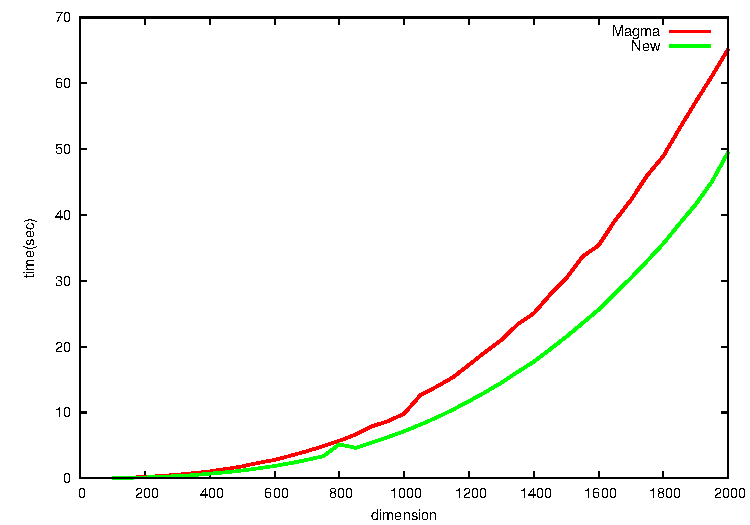
\includegraphics[width = 10cm]{figures/MMtiming.pdf}
\end{center}
\caption{\small Matrix multiplication with bitsize 200}
\label{figure:MMtiming}
\end{figure}

A natural way of computing $\Psi$ is to simply iterate over all entries of the input matrix and 
reduce each entry module each prime $p_i$ by a fast reduction function. But a more clever way is to 
do reduction by matrix multiplication as follows. Let $v = (t_1, t_2, \cdots, t_n)$ be a row of the 
matrix $A$. Write $t_i = t_{i1}t_{i2}\cdots t_{ir}$ in a basis of the form $\omega = 2^d$. Then 
compute
\[
C = 
 \begin{pmatrix}
  \omega^r \pmod {p_1} & \omega^{r - 1} \pmod {p_1} & \cdots &  1\\
  \omega^r \pmod {p_2} & \omega^{r - 1} \pmod {p_2} & \cdots &  1\\
  \vdots  & \vdots  & \ddots & \vdots  \\
  \omega^r \pmod {p_k} & \omega^{r - 1} \pmod {p_k} & \cdots &  1\\
 \end{pmatrix}
 \begin{pmatrix}
  t_{11} & t_{21} & \cdots & t_{n1} \\
  t_{12} & t_{22} & \cdots & t_{n2} \\
  \vdots  & \vdots  & \ddots & \vdots  \\
  t_{1r} & t_{2r} & \cdots & t_{nr} \\
 \end{pmatrix}
\]
The $i$th, $1 \le i \le k$, row of the matrix $C$ is the row $v$ reduced mod $p_i$. The same thing 
can be done for all rows of $A$ to compute the tuple $(A_1, \dots, A_k)$. The Vandermonde like 
matrix of $\omega^i$ is precomputed.

If the entries of the input matrices are very large then the value $x = \sum_{i = 1}^k a_it_iM_i$ in 
\refstep{step:gauss-minv} of  \refalgorithm{algorithm:lZMul} can be computed by a divide and conquer 
algorithm \cite{VonzurGathen1999}: Let $\alpha = p_{k / 2 + 1}p_{k / 2 + 2}\cdots p_k$ and $\beta = 
p_1p_2\cdots p_{k / 2}$ then
\begin{eqnarray*}
x & = & \alpha(a_1t_1M_1/\alpha + \cdots + a_{k / 2}t_{k / 2}M_{k / 2}/\alpha) \\
& & + \beta(a_{k / 2 + 1}t_{k / 2 + 1}M_{k / 2 + 1}/\beta + \cdots + a_kt_kM_k/\beta)
\end{eqnarray*}
All the values $\alpha$ and $\beta$ are precomputed. Another way of computing $x = \sum_{i = 1}^k 
a_it_iM_i$ is using a similar matrix multiplication technique as above with $t_i$ replaced by $M_i$. 
Figure \ref{figure:MMtimingDetail} shows a timing for different phases of 
\refalgorithm{algorithm:labsMMul} where \verb|reduction|, \verb|residue mul|, and \verb|inverse| are 
steps \{\ref{step:Mn-reduction1}, \ref{step:Mn-reduction2}\}, \ref{step:Mn-resmul}, and 
\ref{step:Mn-inverse} of the algorithm respectively.

\begin{figure}[ht]
\setlength{\abovecaptionskip}{-0.5cm}
%\setlength{\belowcaptionskip}{0cm}
\begin{center}
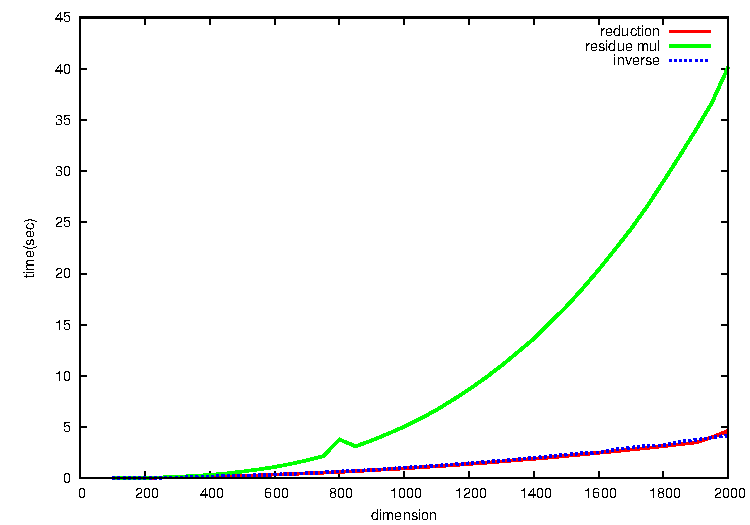
\includegraphics[width = 10cm]{figures/MMtimingDetail.pdf}
\end{center}
\caption{\small Multiplication phases with bitsize 200}
\label{figure:MMtimingDetail}
\end{figure}










\section{Some computational speed-ups}
\label{section:MMapll}

Matrix multiplication is the building block of many computational algorithms. Therefore, having a 
fast matrix multiplication library results in a speed-up in many computational areas. In this 
section, we present some specific problems, required in subsequent chapters, and show how to have 
major speed-ups by giving new implementations of the solutions based on matrix multiplication.

\paragraph{Modular Polynomial Composition.}
Let $F$ be a field and let $p(x) = p_0 + p_1x + \cdots + p_nx^n$, $q(x) = q_0 + q_1x + \cdots + 
q_nx^n$, and $f(x)$ be polynomials in $F[x]$. Then the problem is to compute $p(q) \text{ mod } f$. 
Here, we implement an algorithm by Brent and Kung \cite{BreKun1978} which was proposed for 
computation of the first $n \in \vmathbb{N}_{\ge 1}$ coefficients of the composition of two formal 
power series. But it also works for polynomial composition modulo an arbitrary polynomial $f(x)$.
\begin{algorithm}
[Modular Polynomial Composition]
\label{algorithm:polyComp}
\begin{algorithmic}[1]
\REQUIRE  polynomials $p, q, f \in F[x]$
\ENSURE  $q(p) \text{ mod } f$
\STATE $k \leftarrow \lceil \sqrt{n + 1} \rceil$
\STATE write $q(x) = Q_0(x) + Q_1(x)x^k + \cdots + Q_{k - 1}(x)(x^k)^{k - 1}$
\STATE compute $p^i(x), \: i = 2, \dots, k$
\label{step:BK-pi}
\STATE let $T(s) = p^k(x)$ and compute $T^i(x), \: i = 2, \dots, k - 1$
\label{step:BK-Ti}
\STATE compute $Q_i(p(x)), \: i = 0, \dots, k - 1$ from the \refstep{step:BK-pi}.
\label{step:BK-Qi}
\STATE compute $Q_i(p(x))T^i(x), \: i = 1, \dots, k - 1$ from the steps \ref{step:BK-Ti} and 
\ref{step:BK-Qi}.
\label{step:BK-QiTi}
\STATE compute $h(x) = \sum_{i = 0}^{k - 1} Q_i(p(x))T^i(x)$ from \refstep{step:BK-QiTi}.
\RETURN $h(x)$
\end{algorithmic}
\end{algorithm}
Note that all computations of \refalgorithm{algorithm:polyComp} are done modulo $f(x)$. Let $p^j(x) 
= \sum_{l = 0}^n p_l^{(j)}x^l$, $j = 0, \dots, k$. Then 
$$
Q_i(p(x)) = \sum_{j = 0}^{k - 1} q_{ik + j} \sum_{l = 0}^n p_l^{(j)}x^l = \sum_{l = 0}^n \left(  
\sum_{j = 0}^{k - 1} q_{ik + j}p_l^j\right)x^l
$$
which is essentially the following matrix multiplication.
\[
 \begin{pmatrix}
  p_0^{(0)} & p_0^{(1)} & \cdots & p_0^{(k - 1)} \\
  p_1^{(0)} & p_1^{(1)} & \cdots & p_1^{(k - 1)} \\
  \vdots  & \vdots  & \ddots & \vdots  \\
  p_n^{(0)} & p_n^{(1)} & \cdots & p_n^{(k - 1)}
 \end{pmatrix}
 \begin{pmatrix}
  q_0 & q_k & \cdots & q_{(k - 1)k} \\
  q_1 & q_{k + 1} & \cdots & q_{(k - 1)k + 1} \\
  \vdots  & \vdots  & \ddots & \vdots  \\
  q_{k - 1} & q_{2k - 1} & \cdots & q_{k^2 - 1}
 \end{pmatrix}
\]

\begin{figure}[ht]
\setlength{\abovecaptionskip}{-0.5cm}
%\setlength{\belowcaptionskip}{0cm}
\begin{center}
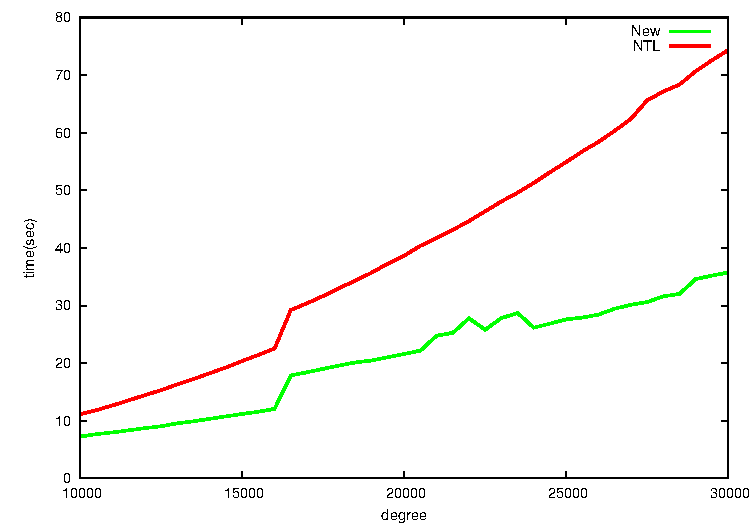
\includegraphics[width = 10cm]{figures/polyCompTiming.pdf}
\end{center}
\caption{\small Modular Polynomial Composition}
\label{figure:polyCompTiming}
\end{figure}

Therefore, \refstep{step:BK-Qi} of \refalgorithm{algorithm:polyComp} can be done using matrix 
multiplication. Let assume that $O(n^\omega)$ is the achievable bound for multiplication of two $n 
\times n$ matrices. For the classical matrix multiplication $\omega = 3$, and for the best known 
algorithm $\omega = 2.37$ \cite{Coppersmith1990}. Except \refstep{step:BK-Qi}, all steps of the 
algorithm can be done in $O(kM(n)) = O(\sqrt{n}M(n))$ multiplications in $F$. Multiplication of the 
matrices of size $n \times \sqrt{n}$ and $\sqrt{n} \times \sqrt{n}$ in \refstep{step:BK-Qi} is 
indeed equivalent to $\sqrt{n}$ multiplications of square matrices of dimension $\sqrt{n} \times 
\sqrt{n}$, which can be done in $O(\sqrt{n}n^{\omega / 2}) = O(n^{(\omega + 1) / 2})$ operations in 
$F$. Therefore, the running time of \refalgorithm{algorithm:polyComp} is $O(\sqrt{n}M(n) + 
n^{(\omega + 1) / 2})$ operations in $F$. So, assuming $M(n) = O(n\log n \log\log n)$, and $\omega = 
2.37$, the best running time for modular composition is $O(n^{1.69})$.\footnote{Huang and Pan 
\cite{Huang1997} showed that for the special dimensions $\sqrt{n} \times \sqrt{n}$ times $\sqrt{n} 
\times n$, $\omega \le 1.67$. So for their algorithm $C(n) = O(n^{1.67})$.} A new implementation of 
the polynomial composition using our matrix multiplication algorithm has been embedded into NTL. 
Figure \ref{figure:polyCompTiming} compares the new and the old algorithm for modular polynomial 
composition in NTL. 

Now that we have a fast modular polynomial composition we briefly show how to use it in polynomial 
factorization over finite fields. Let us first briefly review a factorization method. Let $f(x) \in 
\vmathbb{F}_q[x]$ be of degree $n$, where $q = p^m$ and $\vmathbb{F}_q$ is represented as the quotient 
$\vmathbb{F}_p[y]/g(y)$ with $g(y) \in \vmathbb{F}_p[y]$ monic irreducible of degree $m$. An efficient 
way of factoring $f$ over $\vmathbb{F}_q$ is breaking the factoring into three steps:
\begin{enumerate}
\item \emph{squarefree factorization}: taking the square-free part of $f$;
\label{item:sqf-factor}
\item \emph{distinct-degree factorization}: splitting the square-free polynomial into polynomials 
whose irreducible factors have the same degree;
\item \emph{equal-degree factorization}: completely factoring the square-free polynomial whose 
irreducible factors have the same degree.
\end{enumerate}
The cost of \refstep{item:sqf-factor}, which is done by Yun's algorithm \cite{Yun1976}, is 
$O(M(n)\log n + n\log (q / p))$ operations in $\vmathbb{F}_q$ which is dominated by the cost of other 
steps. So, let assume $f$ is squarefree. The distinct-degree factorization is based on the fact that 
$x^{q^d} - x$ is the product of all monic irreducible polynomials of degree dividing $d$. So, taking 
$\gcd(x^{q^d} - x, f)$ isolates all factors of degree $d$ of $f$. This idea is attributed to Arwin 
\cite{Arwin1918}.

\begin{algorithm}
[Distinct-degree factorization]
\label{algorithm:DDF}
\begin{algorithmic}[1]
\REQUIRE A squarefree monic polynomial $f \in \vmathbb{F}_q[x]$ of degree $n$
\ENSURE The distinct-degree decomposition of $f$
\STATE $f_0 \leftarrow f$, $s \leftarrow \lceil \frac{n}{2} \rceil$
\FOR{$i$ from $1$ to $s$}
	\STATE $h \leftarrow x^{q^i} \text{ mod } f$
	\STATE $g_i \leftarrow \gcd(h - x, f_i)$
	\STATE $f_i \leftarrow \frac{f_{i - 1}}{g_i}$
\ENDFOR
\RETURN $(g_1, \cdots, g_s)$
\end{algorithmic}
\end{algorithm}

Each $g_i$ produced by \refalgorithm{algorithm:DDF} is a squarefree product of monic irreducible 
factors of degree $i$ of $f$. The equal-degree factorization takes $g_i$ and splits it into its 
irreducible factors. This is usually done recursively, i.e. the polynomial is split into two parts 
then the same is done for each of the two parts and so on. The idea, which is due to 
\cite{CantorandZassenhaus1981}, is as follows. Let $f \in \vmathbb{F}_q[x]$ be a squarefree monic 
polynomial of degree $n$ with $\ell = n / d$ irreducible factors $f_i, \: i = 1, \dots, \ell$ of 
degree $d$. Then
$$
\vmathbb{F}_q[x] / \langle f \rangle \cong \prod_{i = 1}^{\ell} \vmathbb{F}_q[x] / \langle f_i \rangle 
\cong \vmathbb{F}_{q^d}^\ell
$$
which induces the mapping 
$$
\setlength\arraycolsep{2pt}
\begin{array}{llll}
\sigma: & \vmathbb{F}_q[x] / \langle f \rangle & \longrightarrow & \{-2, 0\}^{\ell}\\
& a & \longmapsto & (a_1, \dots, a_{\ell})
\end{array}
$$
where $a_i = a^{(q^d - 1) / 2} - 1 \text{ mod } f_i$. Assume $\beta \in \vmathbb{F}_q[x] / \langle f 
\rangle$ is selected at random, and $\sigma(\beta) = (\beta_1, \dots, \beta_\ell)$. If $g = 
\gcd(\beta, f) \ne 1$ then $g$ is a nontrivial factor of $f$; otherwise $\gcd(\beta, f) = 1$, and 
$\gcd(\beta^{(q^d - 1) / 2} - 1, f)$ is a nontrivial factor of $f$ unless $\beta_1 = \beta_2 = 
\dots, = \beta_\ell$ \footnote{If $\beta$ is selected uniformly at random then $\beta_i = -1$ or $1$ 
with probability $1/2$. So, $\beta_1 = \beta_2 = \dots, = \beta_\ell$ occurs with probability 
$2^{-\ell + 1}$.}. 

\begin{algorithm}
[Equal-degree splitting]
\label{algorithm:EDS}
\begin{algorithmic}[1]
\REQUIRE A squarefree monic polynomial $f \in \vmathbb{F}_q[x]$ of degree $n$ and a divisor $d$ of 
$n$ such that all irreducible factors of $f$ have degree $d$.
\ENSURE a proper monic factor of $f$ or "failure"
\STATE $\beta \leftarrow$ a nonconstant random element of $\vmathbb{F}_q[x]$ of degree less than $n$
\STATE $g \leftarrow \gcd(\beta, f)$
\IF {$g \ne 1$} 
	\RETURN $g$ 
\ENDIF
\STATE $g \leftarrow \gcd(\beta^{(q^d - 1) / 2} - 1 \text{ mod } f, f)$
\label{step:EDS-main}
\IF {$g \ne 1, f$} 
	\RETURN $g$ 
\ELSE
	\RETURN "failure"
\ENDIF
\end{algorithmic}
\end{algorithm}
 
The costliest part of \refalgorithm{algorithm:EDS} is \refstep{step:EDS-main}. We show how to 
compute $\beta^{(q^d - 1) / 2} - 1 \text{ mod } f$ efficiently. Let $\lambda \in \vmathbb{F}_q[x]$, 
and assume we are asked to compute $\alpha_k = \lambda^{1 + p + p^2 + \cdots + p^k} \text{ mod } f$ 
for a given integer $k > 0$. Let $\delta_i = \lambda^{p + p^2 + \cdots + p^i} \text{ mod } f$, 
$\zeta_i = x^{p^i} \text{ mod } f$, and $\xi_i = y^{p^i}  \text{ mod } g(y)$. Then we have the 
following recurrence relations
$$
\delta_i = 
\begin{cases}
\delta_{i / 2}\delta_{i / 2}^{p^{i / 2}} & \text{if } i \overset{2}{\equiv} 0 \\
\delta_1\delta_{i - 1}^p & \text{if } i \overset{2}{\equiv} 1 \\
\delta_1 = \lambda^p
\end{cases}
\qquad
\zeta_i = 
\begin{cases}
\zeta_{i / 2}^{p^{i / 2}} & \text{if } i \overset{2}{\equiv} 0 \\
\zeta_{i - 1}^p & \text{if } i \overset{2}{\equiv} 1 \\
\zeta_1 = x^p
\end{cases}
\qquad
\xi_i =
\begin{cases}
\xi_{i / 2}^{p^{i / 2}} & \text{if } i \overset{2}{\equiv} 0 \\
\xi_{i - 1}^p & \text{if } i \overset{2}{\equiv} 1 \\
\xi_1 = y^p
\end{cases}
$$
The initial values $\delta_1$, $\zeta_1$, and $\xi_1$ are computed using the usual exponentiation 
algorithm at a total cost of $O(M(n)M(m)\log p)$ operations in $\vmathbb{F}_p$. Assume, inductively, 
that we have computed $\delta_r$, $\zeta_r$, and $\xi_r$. Then 
\begin{align*}
\delta_r^{p^r} = \left( \sum_{j = 0}^{n - 1} a_j(y)x^j \right)^{p^r} 
& = \sum_{j = 0}^{n - 1} a_j(y)^{p^r}(x^j)^{p^r} = \sum_{j = 0}^{n - 1} a_j(y^{p^r})(x^{p^r})^j\\
& = \sum_{j = 0}^{n - 1} a_j(\xi_r)\zeta_r^j \text{ mod } \langle f(x), g(y) \rangle
\end{align*}
This means that $\delta_{2r}$ and $\delta_{2r + 1}$ can be computed using $O(n)$ modular 
compositions over $\vmathbb{F}_p$, which totally costs $O(nC(m))$ operations in $\vmathbb{F}_p$, and 
$O(1)$ modular multiplications and modular compositions over $\vmathbb{F}_q$, which totally costs 
$O(C(n)M(m))$ operations in $\vmathbb{F}_p$. The values $\zeta_{2r}$ and $\zeta_{2r + 1}$ are 
computed similarly. The cost of computing $\xi_{2r}$ and $\xi_{2r + 1}$ is dominated by the above. 
Therefore, $\delta_k$ and hence $\alpha_k = \lambda\delta_k$ can be computed using $O(\log 
k(M(n)M(m)\log p + nC(m) + C(n)M(m)))$ operations in $\vmathbb{F}_p$. Now, let $\lambda = \beta^{(p - 
1) / 2}$ then
$$
\beta^{(q^d - 1) / 2} = \beta^{(p^{md} - 1) / 2} = \left( \beta^{(p - 1) / 2} \right)^{1 + p + p^2 + 
\cdots + p^{md - 1}} = \lambda^{1 + p + p^2 + \cdots + p^{md - 1}} \text{ mod } \langle f(x), g(y) 
\rangle
$$
which can be computed at a cost of $O(\log(md)(M(n)M(m)\log p + nC(m) + C(n)M(m)))$ operations in 
$\vmathbb{F}_p$. The above idea of using modular composition for raising to the powers of the 
characteristic is essentially due to Kaltofen and Shoup \cite{KaltofenShoup1997}.

To speed the distinct-degree factorization up, \refalgorithm{algorithm:DDF}, the values $x^q, 
x^{q^2}, \dots, x^{q^s}$ can be computed at once. For this, we first compute $x^q = x^{p^m}$ using 
the above algorithm and then compute $x^{q^2}, \dots, x^{q^s}$ using the algorithm introduced in 
\cite{zurShoup1992}. 

\paragraph{Power Projection.}
Let $f \in \vmathbb{F}_p[x]$ with $\deg f = n$. Given $g \in \vmathbb{F}_p[x]/(f)$, and the vector $v 
\in \vmathbb{F}_p^n$, the problem is to compute the sequence
\begin{equation}
\label{equation:powp}
\langle v, 1\rangle, \langle v, g\rangle , \dots, \langle v, g^{m - 1} \rangle
\end{equation}
for a positive integer $m$; Here, $\langle ., .\rangle$ is the inner product operator. Let $h\circ v 
\in \vmathbb{F}_p^n$ be the unique vector such that $\langle h\circ v, \alpha \rangle = \langle v, 
h\alpha \rangle$ for all $\alpha \in \vmathbb{F}_p[x]/(f)$. Sequence (\ref{equation:powp}) can be 
computed by \refalgorithm{algorithm:powerp} due to Shoup \cite{Shoup1999}. \refstep{step:powerp-for} 
of the algorithm can be replaced by a matrix multiplication. As in the case of polynomial 
composition, this new power projection algorithm has been embedded into NTL. Figure 
\ref{figure:powerp} compares the performance of the old and the new algorithm.

\begin{algorithm}
[Power Projection]
\label{algorithm:powerp}
\begin{algorithmic}[1]
\REQUIRE  $v \in \vmathbb{F}_p^n, f  \in \vmathbb{F}_p[x], g \in \vmathbb{F}_p[x]/(f)$
\ENSURE   The sequence $\langle v, 1\rangle, \langle v, g\rangle , \dots, \langle v, g^{m - 1} 
\rangle$
\STATE $k \leftarrow \lfloor l^{1/2} \rfloor, \: k^\prime \leftarrow \lceil l/k \rceil$
\FOR{$i$ from $0$ to $k^\prime - 1$}
\label{step:powerp-for}
	\STATE $c_{ik + j} \leftarrow \langle v, g^j\rangle \quad (0 \le j < k)$
	\STATE $v \leftarrow g^k \circ v$
\ENDFOR
\RETURN $c_0, \dots, c_{m - 1}$
\end{algorithmic}
\end{algorithm}

\begin{figure}[ht]
\setlength{\abovecaptionskip}{-0.5cm}
%\setlength{\belowcaptionskip}{0cm}
\begin{center}
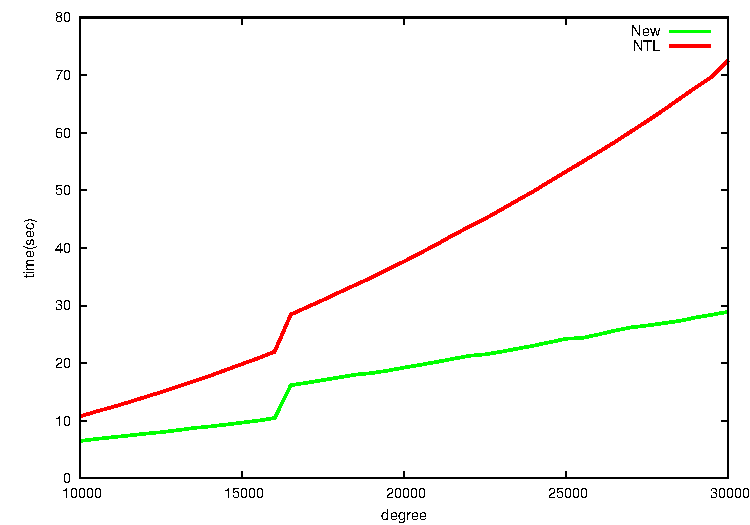
\includegraphics[width = 10cm]{figures/powerProjectTiming.pdf}
\end{center}
\caption{\small Power Projection}
\label{figure:powerp}
\end{figure}




\chapter{Computing Roots Over Finite Fields}
\label{chapter:rootcomp}

Let $R$ be a ring and let $a \in R$. Computing $a^{1/n}$, where $n$ is an integer, beside its 
intrinsic interest, is of great importance in many areas of mathematics and computer science. This 
problem can equivalently be considered as finding a root of $x^n - a \in R[x]$ in some extension of 
$R$. In this chapter, we focus on the cases where $R$ is a finite field, and devote some more space 
to the case $n = 2$ which is of special interest in point counting and cryptography. The first two 
sections are preliminary for subsequent sections. We first present some square root algorithms, and 
then extend them to compute higher roots.



\section{Discrete logarithm in cyclic $p$-groups}
\label{section:dlp-cpgroups}

A finite $p$-group $G$ is a group of order $n = p^m$ where $p$ is a prime. A special case of the 
discrete logarithm problem occurring in root computation is the one in finite cyclic $p$-groups. The 
algorithm we present here is due to Pohlig and Hellman \cite{Pohlig1978}. Let $g, a \in G$ with $g$ 
a generator of $G$. The problem is to find the integer $0 \le x \le n - 1$ such that $g^x = a$. 
Suppose that $x$ has the expansion $x = \sum_{i = 0}^{m - 1}x_ip^i, \: 0 \le x_i \le p - 1$ in base 
$p$. Then
\begin{equation}
\label{equation:dlp-dh}
a^{\frac{n}{p}} = g^{x\frac{n}{p}} = (g^{\frac{n}{p}})^x = (g^{\frac{n}{p}})^{\sum_{i = 0}^{m - 
1}x_ip^i} = (g^{\frac{n}{p}})^{x_0} = \zeta^{x_0}
\end{equation}
where $\zeta = g^{\frac{n}{p}}$ is a primitive $p$-th root of unity. Therefore, $x_0$ is uniquely 
determined by (\ref{equation:dlp-dh}). Let assume $x_1, \dots, x_k, \: k < m$ are determined. Then 
$$
(ag^{-\sum_{i = 0}^{k}x_ip^i})^{n / p^{k + 2}} = (g^{\frac{n}{p}})^{x_{k + 2}} = \zeta^{x_{k + 2}}
$$
so that $x_{k + 1}$ is uniquely determined, and hence $x$ is determined by induction. When $p$ is 
small, the values $0 \le x_i \le p - 1$ can be found by a brute force search. But when $p$ is large, 
one can use techniques like Shank's baby-step giant-step \cite{Shank1971} and Pollard's rho method 
\cite{Pollard1978}. The baby-step giant-step algorithm needs memory for $O(\sqrt{p})$ group 
elements, and its running time is $O(\sqrt{p})$ group multiplications; while the running time of the 
Pollard's rho method is the same, but it requires a negligible amount of memory. The expected 
running time of the above algorithm, which requires $m$ exponentiations and applications of, say 
Pollard's method, for discrete logarithm in $G$ is $O(m(\log_2{n} + \sqrt{p}))$ group 
multiplications.







\section{Randomized search for irreducible polynomials}
\label{section:r-s-irr-poly}

In this section, we briefly discuss the asymptotic probability for a randomly selected polynomial, 
with prescribed constraints, to be irreducible over a finite field. Let $N(n, q)$ denote the number 
of monic irreducible polynomials of degree $n$ over $\vmathbb{F}_q$. It is not hard to prove that 
$$
N(n, q) = \frac{1}{n}\sum_{d \mid n}\mu(d)q^{\frac{n}{d}}
$$
where $\mu$ is the M\"obius function. This formula was discovered by Gauss \cite{Gauss1981} for the 
case $q = p$. There are $q^n$ monic polynomials of degree $n$ over $\vmathbb{F}_q$. So, the 
probability $P(n, q)$ for a uniformly random monic polynomial of degree $n$ to be irreducible is 
$N(n, q) / q^n$. The following lemma shows that $P(n, q) \in \Theta(\frac{1}{n})$.
\begin{lemma}
The number $N(n, q)$ of monic irreducible polynomials of degree $n$ over $\vmathbb{F}_q$ satisfies
$$
\frac{1}{n}q^n - \frac{q}{n(q - 1)}(q^{\frac{n}{2}}) \le N(q, n) \le \frac{1}{n}(q^n - q) \qquad n 
\ge 2
$$
with equality on the right if and only if $n$ is prime.
\end{lemma}
\begin{proof}
The equality on the right is trivial when $n$ is prime. By the M\"obius inversion 
$$
q^n = \sum_{d \mid n}dN(d, q) = nN(n, q) + q + \sum_{\substack{d \mid n \\ d \ne 1, n}}dN(d, q) \ge 
nN(n, q) + q
$$
which establishes the upper bound. Once we proved the upper bound it can be used to prove the lower 
bound:
\begin{align*}
q^n = \sum_{d \mid n}dN(d, q) 
&= nN(n, q) + \sum_{\substack{d \mid n \\ d \ne n}}dN(d, q) \\
&\le nN(n, q) + \sum_{d = 1}^{n / 2} q^d = nN(n, q) + q \frac{q^{\frac{n}{2}} - 1}{q - 1} \qedhere
\end{align*}
\end{proof}
The coefficient of $x^{n - 1}$ of the monic polynomial $f$ of degree $n$ is called the trace of $f$. 
Let $N_\gamma(n, q)$ denote the number of polynomials of degree $n$ and trace $\gamma$ over 
$\vmathbb{F}_q$. Carlitz \cite{Carlitz1952} showed that
$$
N_\gamma(n, q) = \frac{1}{qn}\sum_{\substack{d \mid n \\ p \nmid d}} \mu(d)q^{\frac{n}{d}} \qquad 
\gamma \ne 0
$$
which means that $N_\gamma(n, q)$ does not depend on the trace $\gamma$. Let $n = p^km$ with $p 
\nmid m$. Then 
$$
N_0(n, q) = \frac{1}{qn}\sum_{d \mid m} \mu(d)q^{\frac{n}{d}} - \frac{\varepsilon}{n}\sum_{d \mid 
m}\mu(d)q^{\frac{n}{dp}} \qquad \gamma \ne 0
$$
where $\varepsilon = 1$ if $k > 0$ and $\varepsilon = 0$ if $k = 0$ \cite{Yucas2006}. Let $N(n, c, 
q)$ denote the number of monic irreducible polynomial of degree $n$ and constant term $c$. Let $D_n 
= \{r : r \mid q^n - 1, r \nmid q^m - 1 \text{ for } m < n\}$, and let $\lambda$ be the order of 
$c$. For each $r \in D_n$ let $r = m_rd_r$ where $d_r = \gcd(r, (q^n - 1)/(q - 1))$. An explicit 
formula for $N(n, c, q)$ was obtained in \cite{Yucas2006} as follows.
\begin{equation}
\label{equation:irr-const}
N(n, c, q) = \frac{1}{n\varphi(\lambda)}\sum_{\substack{r \in D_n \\ m_r = \lambda}} \varphi(r)
\end{equation}
where $\varphi$ is the Euler's function. Following the same notation as above let $N_\gamma(n, c, 
q)$ denote the number of irreducible polynomials of degree $n$, trace $\gamma$, and constant term 
$c$. The following bound was established by Wan \cite{Wan1997}. See \cite{Moisio2007} for an 
improvement to this bound.
\begin{equation}
\label{equation:irr-const-bound}
\left| N_\gamma(n, c, q) - \frac{q^{n - 1}}{n(q - 1)}\right| \le \frac{3}{n}q^{n / 2}
\end{equation}
Let $P(n, c, q)$ denote the probability for a uniformly random monic polynomial of degree $n$ and 
constant term $c$ to be irreducible. 
Summing both sides of (\ref{equation:irr-const}) over all elements of $\vmathbb{F}_q$ we have
\begin{align*}
\frac{3}{n}q^{(n + 2) / 2} = \sum_{\gamma \in \vmathbb{F}_q}\frac{3}{n}q^{n / 2} 
& \ge \sum_{\gamma \in \vmathbb{F}_q} \left| N_\gamma(n, c, q) - \frac{q^{n - 1}}{n(q - 1)}\right| \\
& \ge \left| \sum_{\gamma \in \vmathbb{F}_q}N_\gamma(n, c, q) - \sum_{\gamma \in 
\vmathbb{F}_q}\frac{q^{n - 1}}{n(q - 1)}\right| \\
& = \left| N(n, c, q) - \frac{q^n}{n(q - 1)}\right|
\end{align*}
Since the number of all polynomials of degree $n$ and a prescribed constant term is $q^{n - 1}$, the 
above bound shows that $P(n, c, q) \in \Theta(\frac{1}{n})$. This means that for a monic polynomial 
$f \in \vmathbb{F}_q[x]$ of degree $n$, if the constant term is fixed and all other coefficients are 
selected in a uniformly random way then there still is a reasonable chance for $f$ to be 
irreducible. The surprising fact is that the above asymptotic results hold for some polynomials of 
very special form. Extensive research has been done on the number of irreducible binomials and 
trinomials over finite fields. These polynomials are very computationally useful, and result in 
simpler representations of extensions of finite fields. 

Let $T_n(p)$ be the number of irreducible polynomials of the form $x^n + x + a \in \vmathbb{F}_p[x]$ 
over $\vmathbb{F}_p$. Then $T_n(p)$ is asymptotic to $p / n$ for a fixed $n$ and $p \rightarrow 
\infty$. This was first conjectured by Chowla \cite{Chowla1966}. The following more general result 
was proved by Cohen \cite{Cohen1970} and Ree \cite{Ree1971}. 
\begin{theorem}
For an integer $n$ such that $p \nmid n(n - 1)$, let $T_n(q)$ denote the number of trinomials $x^n + 
x + a \in \vmathbb{F}_q[x]$ that are irreducible over $\vmathbb{F}_q$. Then
$$
\left| T_n(q) - \frac{q}{n} \right| \le C_nq^{\frac{1}{2}}
$$
where $C_n$ is a constant depending only on $n$.
\end{theorem}









\section{General approaches}

There are many polynomial factorization algorithms that can be used as general algorithms to find an 
$n$th root of an element of a finite field. See \cite{vonzurGathen2001} for a survey of polynomial 
factorization over finite fields and \cite{Lidl-Niederreiter1994} for special root finding 
algorithms based on factorization. For an element $a \in \vmathbb{F}_q$ if $\sqrt[n]{a} \notin 
\vmathbb{F}_q$ then there is a finite extension $\vmathbb{F}_{q^m} / \vmathbb{F}_q$ containing 
$\sqrt[n]{a}$. Therefore, given $a \in \vmathbb{F}_q$, we can always assume that an $n$-th root of 
$a$ is contained in $\vmathbb{F}_q$, since a polynomial over $\vmathbb{F}_q$ can always be viewed as a 
polynomial over $\vmathbb{F}_{q^m}$. Let $f \in \vmathbb{F}_q[x]$ be an arbitrary polynomial. To find 
the zeros of $f$ in $\vmathbb{F}_q$, it is sufficient to apply the equal degree factorization 
algorithm to $\gcd(x^q - x, f)$.

\begin{algorithm}
[Root finding using factorization]
\label{algorithm:groot1}
\begin{algorithmic}[1]
\REQUIRE A nonconstant $f \in \vmathbb{F}_q[x]$
\ENSURE  Zeros of $f$ in $\vmathbb{F}_q$
\STATE $h \leftarrow x^q \mod f$.
\label{step:genroot-pow}
\STATE $g \leftarrow \gcd(h - x, f), d \leftarrow \deg{g}$
\label{step:genroot-gcd}
\IF {$d = 0$} 
	\RETURN $\varnothing$
\ENDIF
\STATE factorize $g$ using equal degree factorization to get the linear factors $x - u_i, \: i = 1, 
\dots, d$
\RETURN $u_i, \: i = 1, \dots, d$
\end{algorithmic}
\end{algorithm}

\refalgorithm{algorithm:groot1} can be applied to the polynomial $x^n - a$ to compute an $n$-th root 
of $a$. It is essentially due to Legendre \cite{Legendre1785}. He suggested, in the case $q = p$, 
splitting $\gcd(f, x^{p - 1} - 1)$ by computing $\gcd(f, x^{(p - 1) / 2} \pm 1)$ and substituting 
$x$ by $x + a$ for a random $a \in \vmathbb{F}_p$ in the case of a trivial split. The dominant steps 
of the algorithm are steps \ref{step:genroot-pow} and \ref{step:genroot-gcd} which take 
$O(M(n)\log{q})$ and $O((\log{q} + \log{n})M(n)\log{n})$ operations in $\vmathbb{F}_q$ respectively. 
Therefore, the running time is $O(M(n)\log{n}\log(nq))$ or $\tilde{O}(n\log{q})$ operations in 
$\vmathbb{F}_q$.








\section{Computing square roots}
\label{section:squareroot}

Let $G$ be a group with an odd order $n$. Then the mapping $f: G \rightarrow G$, $f(x) = x^2$ is an 
automorphism of $G$, hence every element $x \in G$ has a unique square root which is $x^{(n + 
1)/2}$. For the cyclic group $\vmathbb{F}_q^*$ if $q = 2^m$ then the square root of $x \in 
\vmathbb{F}_q^*$ is $x^{2^{n - 1}}$. In fact, this is true in general, i.e. for $q = p^n$ the $p$-th 
root of $x \in \vmathbb{F}_q^*$ is $x^{p^{n - 1}}$. If $q \equiv 3 \pmod 4$ then for any $x \in 
(\vmathbb{F}_q^*)^2$ the square root is $x^{(q + 1) / 4}$. The latter is because $(\vmathbb{F}_q^*)^2$ 
is a subgroup of odd order $(q - 1) / 2$.

An interesting field theoretic approach to computing square roots in $\vmathbb{F}_q$ was introduced 
by Cipolla \cite{Cipolla1903}. Let $K = \vmathbb{F}_{q^m}$ be a finite extension of $\vmathbb{F}_q$, 
and let $N_{K/\vmathbb{F}_q}: K \rightarrow \vmathbb{F}_q$ be the norm function 
$N_{K/\vmathbb{F}_q}(\alpha) = \prod_{i = 1}^{m - 1}\alpha^{q^i} = \alpha^{(q^m - 1)/(q - 1)}$. Then 
$N_{K/\vmathbb{F}_q}$ is surjective. The idea of Cipolla's algorithm is as follows. Let $a \in 
\vmathbb{F}_q$, and assume we find a quadratic extension $K = \vmathbb{F}_{q^2}$ of $\vmathbb{F}_q$ by 
adjoining a quadratic nonresidue to $\vmathbb{F}_q$. Then, there is an element $x \in K$ such that 
$N_{K/\vmathbb{F}_q}(x) = a$. But $N_{K/\vmathbb{F}_q}(x) = x^{q + 1}$ hence $\sqrt{a} = x^{(q + 1) / 
2}$.

\begin{algorithm}
[Cipolla's square root]
\label{algorithm:Cipolla-sq}
\begin{algorithmic}[1]
\REQUIRE A nonzero $a \in \vmathbb{F}_q$
\ENSURE Square root of $a$ in $\vmathbb{F}_{q^2}$
\STATE choose a random $b \in \vmathbb{F}_q$
\IF {$b^2 - 4a$ is a square} 
	\RETURN failure.
\ENDIF
\STATE $c \leftarrow x^{(q + 1) / 2} \mod x^2 - bx + a$
\label{step:Cipolla-norm}
\RETURN $c$
\end{algorithmic}
\end{algorithm}

If $\left( \frac{b^2 - 4a}{\vmathbb{F}_q}\right) = -1$ then the polynomial $f(x) = x^2 - bx + a$ is 
irreducible over $\vmathbb{F}_q$ hence $\vmathbb{F}_q[x]/(f)$ is a field. Since $f$ is the minimal 
polynomial of $x$ over $\vmathbb{F}_q$, $c^2 = N_{K/\vmathbb{F}_q}(x) = a$. According to 
\refsection{section:r-s-irr-poly}, finding a quadratic nonresidue of the form $b^2 - 4a$ by choosing 
random $b \in \vmathbb{F}_q$, which is equivalent to choosing a uniformly random polynomial of degree 
$2$ and constant term $a$, does not require too many trials. More precisely \cite[page 
158]{BachSh1996},

\begin{lemma}
The probability of $\left(\frac{b^2 - 4a}{\vmathbb{F}_q}\right) = -1$ for a randomly chosen $b \in 
\vmathbb{F}_q$ is $(q - 1)/2q$.
\end{lemma} 

\refalgorithm{algorithm:Cipolla-sq} fails with probability $(q + 1) / 2q$. The quadratic residue 
test, and \refstep{step:Cipolla-norm} take $O(\log q)$ and $O(\log q)$ multiplications in 
$\vmathbb{F}_q$ respectively. Therefore, its expected complexity is $O(\log q)$ multiplications in 
$\vmathbb{F}_q$.

Another algorithm for computing square roots is the algorithm of Tonelli \cite{Tonelli1891}. The 
algorithm, which is more group theoretic, was improved by Shanks \cite{Shanks1972} and is known as 
Tonelli-Shanks algorithm. The idea of the algorithm is to use discrete logarithm to reduce the 
problem to a subgroup of $\vmathbb{F}_q^*$ of an odd order. Let $q - 1 = 2^r\ell$ with $(\ell, 2) = 
1$. Let $H$ be the unique subgroup of $\vmathbb{F}_q^*$ of order $\ell$. Then we have a chain of 
subgroups
$$
H = H_0 \subset H_1 \subset \cdots \subset H_r = \vmathbb{F}_q^*
$$
where $H_i / H_{i - 1}$ is a simple group of order 2 for $i = 1, \dots, r$. The natural homomorphism 
$\vmathbb{F}_q^* \rightarrow \vmathbb{F}_q^* / H$ sends any quadratic nonresidue of $\vmathbb{F}_q^*$ 
to a generator of $\vmathbb{F}_q^* / H$. Assume we find a quadratic nonresidue $g \in 
\vmathbb{F}_q^*$. Then the square root of an element $a \in \vmathbb{F}_q^*$ can be computed as 
follows. We can be express $a$ as $g^th \in g^tH$ by solving a discrete logarithm in $\vmathbb{F}_q^* 
/ H$. Now, $t$ is necessarily even, so that $\sqrt{a} = g^{t / 2}h^{(\ell + 1) / 2}$. Here is the 
algorithm.

\begin{algorithm}
[Tonelli-Shanks square root]
\label{algorithm:Tonelli-sq}
\begin{algorithmic}[1]
\REQUIRE A nonzero $a \in \vmathbb{F}_q$ with $q$ odd
\ENSURE Square root of $a$ in $\vmathbb{F}_{q}$
\STATE choose a random $g \in \vmathbb{F}_q$
\IF {$g$ is a square} 
	\RETURN failure.
\ENDIF
\STATE let $q - 1 = 2^r\ell$ with $2 \nmid \ell$.
\label{step:factor-q}
\STATE let $H$ be the subgroup of $\vmathbb{F}_q^*$ of order $\ell$
\STATE $t \leftarrow $ the discrete logarithm of $aH$ in base $gH$
\label{step:TS-DL}
%\FOR {$i = 2$ \TO $r$}
%	\IF {$(ag^{-t})^{(q - 1) / 2^i} \ne 1$} 
%		\STATE $t \leftarrow 2^{i - 1} + t$ 
%	\ENDIF
%\ENDFOR
\STATE $h \leftarrow ag^{-t}$
\RETURN $g^{t / 2}h^{(\ell + 1) / 2}$
\end{algorithmic}
\end{algorithm}

According to \refsection{section:dlp-cpgroups}, \refstep{step:TS-DL} of 
\refalgorithm{algorithm:Tonelli-sq} requires $O(r^2)$ multiplications in $\vmathbb{F}_q$ where $r$ is 
the highest power of $2$ dividing $q - 1$. All other steps take $O(\log q)$ multiplications in 
$\vmathbb{F}_q$. Hence, the expected running time of the algorithm is $O(r^2 + \log q)$ 
multiplications in $\vmathbb{F}_q$. Despite  \refalgorithm{algorithm:Cipolla-sq}, the efficiency of 
this algorithm depends on the structure of $\vmathbb{F}_q^*$. Let $r$ and $\ell$ be as in 
\refstep{step:factor-q} of the algorithm. For most $q$, $r$ is fairly small \footnote{For example, 
primes used in public-key cryptography, see \cite{Maurer1992a, Maurer1989}.}, and 
\refalgorithm{algorithm:Tonelli-sq} requires few exponentiations in $\vmathbb{F}_q^*$, and hence 
preferred over \refalgorithm{algorithm:Cipolla-sq} which requires exponentiation in 
$\vmathbb{F}_{q^2}$. If $2^r$ is comparable to $\ell$ then the running time of 
\refalgorithm{algorithm:Tonelli-sq} is $O((\log q)^2)$. In this case,  
\refalgorithm{algorithm:Cipolla-sq} is preferable. The latter case can happen quite naturally:
\begin{theorem}
\label{theorem:Dir-ar-prog}
Let $a$ and $b$ be positive coprime integers. Then there are infinitely many primes $p$ such that $p 
\overset{b}{\equiv} a$.
\end{theorem}

This is due to Dirichlet \cite{Dirichlet1837}, and known as \emph{Dirichlet's theorem on arithmetic 
progressions}; Because it equivalently says that if $a$ and $b$ are positive coprime integers then 
the arithmetic progression $a, a + b, a + 2b, \dots$ contains infinitely many primes. Let $p(a, b)$ 
be the least prime in this arithmetic progression. Linnik \cite{Linnik1944} proved that there is a 
constant $L > 0$ such that $p(a, b) < b^L$. This constant is not too large, e.g. it is shown in 
\cite{Heath-Brown1992} that $L \le 11/2$. By  \reftheorem{theorem:Dir-ar-prog}, for any given 
integer $r > 0$, there are infinitely many primes in the progression $1, 1 + 2.2^r, 1 + 3.2^r, 
\dots, 1 + k.2^r, \dots$. Let $q$ be the least prime in this sequence. Then $2^r \mid q - 1$, and $q 
\le 2^{11r/2}$, and hence $2\log q / 11 \le r$. This shows the bound $O((\log q)^2)$ for 
\refalgorithm{algorithm:Tonelli-sq} is tight.

Let $\mathcal{P} = \bigcup_{i \in \vmathbb{N}}\left\lbrace \text{the least prime } p_i \text{ such 
that } p_i \equiv 2^i + 1 \text{ mod } 2^{i + 1} \right\rbrace$. Then $\mathcal{P}$ is clearly not 
finite. Let $\{q_n\}_{n \in \vmathbb{N}}$ be an increasing sequence of elements of $\mathcal{P}$, and 
let $C(q)$ and $T(q)$ be the expected complexity of algorithms \ref{algorithm:Cipolla-sq} and 
\ref{algorithm:Tonelli-sq} respectively, averaged over all quadratic residue and non-residue inputs. 
Then it is not hard to prove, see \cite{Tornaria2002}, that
$$
\lim_{n \to \infty}\frac{T(q_n)}{C(q_n)} = \infty.
$$
which means we have found an infinite sequence of primes for which 
\refalgorithm{algorithm:Cipolla-sq} is asymptotically better.

The last square root algorithm we present is a new algorithm based on the trace function. Assume 
that the field $\vmathbb{F}_q$, where $q = p^n$, is represented, as usual, by a quotient 
$\vmathbb{F}_p[x] / (f(x))$ with $f(x) \in \vmathbb{F}_p[x]$ a monic irreducible polynomial of degree 
$n$. Let $T_{\vmathbb{F}_q / \vmathbb{F}_p}: \vmathbb{F}_q \rightarrow \vmathbb{F}_p$ be the trace 
function $T_{\vmathbb{F}_q / \vmathbb{F}_p}(\alpha) = \sum_{i = 0}^{n - 1} \alpha^{p^i}$ where $\alpha 
\in \vmathbb{F}_q$ . Given $a \in \vmathbb{F}_q^\times$, let $\gamma \in \vmathbb{F}_q$ be a square 
root of it. Then
\begin{equation}
\label{equation:tr-square}
\begin{aligned}
\vmathbb{F}_p \ni \beta = T_{\vmathbb{F}_q / \vmathbb{F}_p}(\gamma) = \sum_{i = 1}^{n - 1} \gamma^{p^i}
& = \gamma(1 + \gamma^{p - 1} + \gamma^{p^2 - 1} + \cdots + \gamma^{p^{n - 1} -1}) \\
& = \gamma(1 + a^{(p - 1) / 2} + a^{(p^2 - 1) / 2} + \cdots + a^{(p^{n - 1} -1) / 2})
\end{aligned}
\end{equation}
Let $b = 1 + a^{(p - 1) / 2} + a^{(p^2 - 1) / 2} + \cdots + a^{(p^{n - 1} -1) / 2}$. We may assume 
$b \ne 0$; because otherwise,  we can start by $ac^2$ for different random elements $c \in 
\vmathbb{F}_q^\times$ until we get a nonzero $b$, and at the end multiply the result by $c^{-1}$. 
Squaring both side of the \refequation{equation:tr-square} results in the quadratic equation 
$\beta^2 = ab^2$ over $\vmathbb{F}_p$ from which $\beta$ can be determined. Then $\gamma = \beta 
b^{-1}$. Computing $\beta$ from the above quadratic equation takes $O(\log p)$ operation in 
$\vmathbb{F}_p$. Therefore, efficient computation of $\gamma$ needs an efficient computation of $b$. 
For this, we use a recursive technique, similar to the one used in  \refsection{section:MMapll}, as 
follows. Let $\lambda \in \vmathbb{F}_q$, and assume we are asked to compute 
$$
\alpha_k = \lambda^{1 + p} + \lambda^{1 + p + p^2} + \cdots + \lambda^{1 + p + p^2 + \cdots + p^k}
$$
for a given integer $k > 0$. Let $\delta_i = \lambda^{p} + \lambda^{p + p^2} + \cdots + \lambda^{p + 
p^2 + \cdots + p^i}$, $\zeta_i = \lambda^{p + p^2 + \cdots + p^i}$, and $\xi_i = x^{p^i}$. Then we 
have the following recurrence relations
$$
\delta_i = 
\begin{cases}
\delta_{i / 2} + \zeta_{i / 2}\delta_{i / 2}^{p^{i / 2}} & \text{if } i \overset{2}{\equiv} 0 \\
\delta_1 + \zeta_1\delta_{i - 1}^p & \text{if } i \overset{2}{\equiv} 1 \\
\delta_1 = \lambda^p
\end{cases}
\qquad
\zeta_i = 
\begin{cases}
\zeta_{i / 2}\zeta_{i / 2}^{p^{i / 2}} & \text{if } i \overset{2}{\equiv} 0 \\
\zeta_1\zeta_{i - 1}^p & \text{if } i \overset{2}{\equiv} 1 \\
\zeta_1 = \lambda^p
\end{cases}
\qquad
\xi_i =
\begin{cases}
\xi_{i / 2}^{p^{i / 2}} & \text{if } i \overset{2}{\equiv} 0 \\
\xi_{i - 1}^p & \text{if } i \overset{2}{\equiv} 1 \\
\xi_1 = x^p
\end{cases}
$$
Assume, inductively, that we have computed $\delta_r$, $\zeta_r$, and $\xi_r$. Then $\delta_r^{p^r} 
= \left( \sum_{j = 0}^{n - 1} a_jx^j \right)^{p^r} = \sum_{j = 0}^{n - 1} a_j(x^j)^{p^r} = \sum_{j = 
0}^{n - 1} a_j(x^{p^r})^j = \sum_{j = 0}^{n - 1} a_j\xi_r^j$ which means that raising $\delta_r$ to 
the power of $p^r$ is indeed computing the modular polynomial composition $\delta_r\circ\xi_r$ over 
$\vmathbb{F}_p$. Thus, ignoring the additions, computing $\delta_{2r}$ and $\delta_{2r + 1}$ costs 
$O(1)$ polynomial multiplications and modular polynomial compositions over $\vmathbb{F}_p$. The same 
can be done for computing $\zeta_{2r}$, $\zeta_{2r + 1}$, $\xi_{2r}$, and $\xi_{2r + 1}$. Therefore, 
$\delta_k$ and hence $\alpha_k = \lambda\delta_k$ can by computed using $O(C(n)\log k)$ operations 
in $\vmathbb{F}_p$. Now, let $\lambda = a^{(p - 1) / 2}$, then $b = 1 + \lambda + \alpha_{n - 2}$. 
Computing $\lambda$ needs $O(M(n)\log p)$ operations in $\vmathbb{F}_p$, and hence computing $b$ 
needs $O(M(n)\log p + C(n)\log n)$ operations in $\vmathbb{F}_p$. Thus, the expected running time of 
the above algorithm for computing a square of an element $a \in \vmathbb{F}_q$ is $O(M(n)\log p + 
C(n)\log n)$ operations in $\vmathbb{F}_p$. 

\begin{figure}[ht]
\setlength{\abovecaptionskip}{-0.5cm}
%\setlength{\belowcaptionskip}{0cm}
\begin{center}
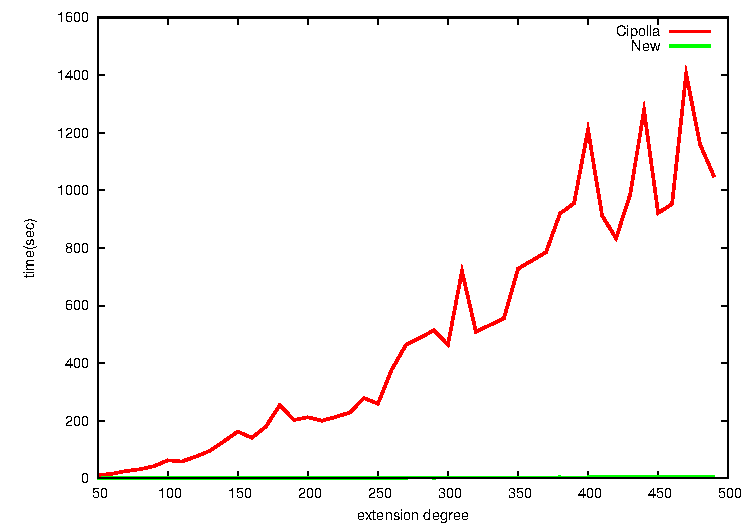
\includegraphics[width = 10cm]{figures/sqrtTiming.pdf}
\end{center}
\caption{\small The new square root algorithm}
\label{figure:sqrtTiming}
\end{figure}

We have implemented the above algorithm, and \refalgorithm{algorithm:Cipolla-sq} in NTL. Figure 
\ref{figure:sqrtTiming} compares the two algorithms in $\vmathbb{F}_q$ with $q = p^n$, for a randomly 
selected prime $p = \seqsplit{348975609381470925634534573457497}$, and different values of the 
extension degree $n$. Since Figure \ref{figure:sqrtTiming} does not reveal the behaviour of the new 
algorithm, a better view of the asymptotic  description of the algorithm for extension degrees $\le 
10000$ is provided in Figure \ref{figure:sqrtTimingHDeg}.

\begin{figure}[ht]
\setlength{\abovecaptionskip}{-0.5cm}
%\setlength{\belowcaptionskip}{0cm}
\begin{center}
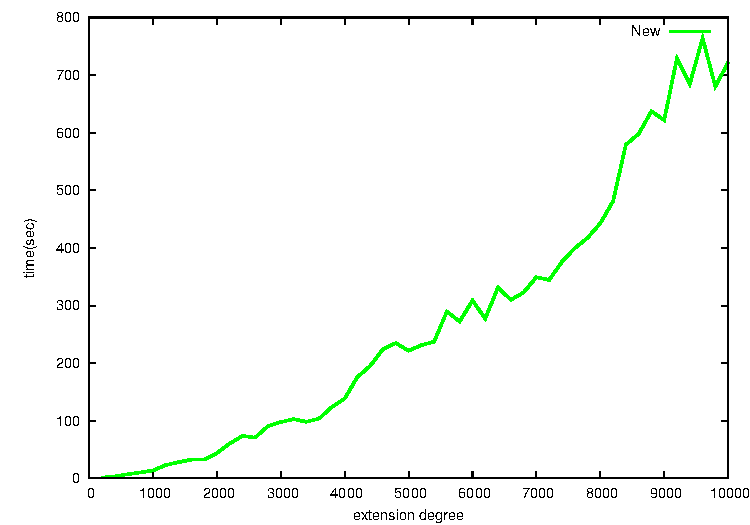
\includegraphics[width = 10cm]{figures/sqrtTimingHDeg.pdf}
\end{center}
\caption{\small The new square root algorithm for high extensions}
\label{figure:sqrtTimingHDeg}
\end{figure}










\section{Computing higher roots}

All of the algorithms presented in \refsection{section:squareroot} for computing square roots can 
somehow be extended to compute $m$-th roots where $m \ge 3$ is an arbitrary integer. In this 
section, we present such extensions, but let us first make the following observation. Let $G$ be a 
group of order $n$ and let $k$ be an integer such that $(n, k) = 1$. Then every $a \in G$ has a 
unique $k$-th root $b = a^{k^{-1} \text{ mod } n}$ in $G$; for if $c$ is another $k$-th root of $a$ 
then $b^k = c^k$ so $(cb^{-1})^k = 1$ which implies $\text{ord}(cb^{-1}) \mid k$ hence 
$\text{ord}(cb^{-1}) \mid (k, n) = 1$. Therefore $cb^{-1} = 1$ hence $c = b$. Suppose we can find a 
$t$-th root of $a \in \vmathbb{F}_q$ when $t$ is a prime divisor of $q - 1$. Then computing an $m$-th 
root of $a$ for an arbitrary $m$ is as follows. Let $m = m_1m_2$ with $(m_2, q - 1) = 1$, and $t 
\mid q - 1$ for every prime divisor $t$ of $m_1$. Then we can compute $a_0 = \sqrt[m_2]{a}$ by 
simply inverting $m_2 \text{ mod } q - 1$. Let $m_1 = \prod_{i = 1}^s{p_i^{\alpha_i}}$ be the prime 
factorization of $m_1$. Then we can compute $a_k = \sqrt[p_1]{a_{k - 1}},\: k = 1, \dots, \alpha_1$ 
and hence $a_{\alpha_1} = \sqrt[p_1^{\alpha_1}]{a_0}$. The same process can be applied to compute 
$\sqrt[p_2^{\alpha_2}]{a_{\alpha_1}}$ and so on. Therefore, the problem is reduced to computing 
$t$-th roots when $t$ is a prime divisor of $q - 1$, and so the algorithms we present in this 
section will compute $t$-th roots for such a $t$.

A natural extension of \refalgorithm{algorithm:Tonelli-sq} was introduced in \cite{AdlManMil1977}. 
Let $t$ be a prime divisor of $q - 1$ and let $q - 1 = t^r\ell$ such that $t \nmid \ell$. As before, 
let $H$ be the unique subgroup of $\vmathbb{F}_q^*$ of order $\ell$. Then we have a chain of 
subgroups
$$
H = H_0 \subset H_1 \subset \cdots \subset H_r = \vmathbb{F}_q^*
$$

where $H_i / H_{i - 1}$ is a simple group of order $t$ for $i = 1, \dots, r$. If $g$ is not a $t$-th 
power then $gH$ generates $\vmathbb{F}_q^*/H$ so that $a$ can be represented as $g^sh$ with $h \in 
H$. Since $a$ is a $t$-th power, it can easily be seen that $t \mid s$. On the other hand $(\left| H 
\right|, t) = 1$. Therefore, a $t$-th root of $a$ is $g^{s/t}h^{t^{-1} \text{ mod } \ell}$. 

\begin{algorithm}
[Tonelli-Shanks $t$-th root when $t$ is a prime divisor of $q - 1$]
\label{algorithm:AMM}
\begin{algorithmic}[1]
\REQUIRE A nonzero $a \in \vmathbb{F}_q$ with $q$ odd
\ENSURE a $t$-th root of $a$ in $\vmathbb{F}_{q}$
\STATE choose a random $g \in \vmathbb{F}_q$
\IF {$g$ is a $t$-th power} 
	\RETURN failure.
\ENDIF
\STATE let $q - 1 = t^r\ell$ with $t \nmid \ell$.
\STATE let $H$ be the subgroup of $\vmathbb{F}_q^*$ of order $\ell$
\STATE $s \leftarrow $ the discrete logarithm of $aH$ in base $gH$
\label{step:AMM-dlog}
\STATE $h \leftarrow ag^{-s}$
\STATE $u \leftarrow t^{-1} \text{ mod } \ell$
\RETURN $g^{s / t}h^u$
\end{algorithmic}
\end{algorithm}

By the following lemma, a randomly chosen $g \in \vmathbb{F}_q$ is a $t$-th power with probability 
$1/t$. Therefore, \refalgorithm{algorithm:AMM} fails with probability $1/t < 1/2$.
\begin{lemma}
Let $G$ be a cyclic group of order $n$. Then $a \in G$ is a $d$-th power if and only if $a^{n/(d, 
n)} = 1$.
\end{lemma}
\begin{proof}
'$\Rightarrow$' is trivial. For the converse let $g$ be a generator of $G$, and $a = g^\ell$. Then 
$1 = a^{n / (d, n)} = g^{\ell n / (d, n)}$. So, $n \mid \ell \frac{n}{(d, n)}$ and hence $(d, n) 
\mid \ell$. Therefore $a = g^\ell = g^{\ell_1(d, n)} = g^{\ell_1(r_1n + s_1d)} = (g^{\ell_1s_1})^d$ 
as desired.
\end{proof}
The expected cost of finding a non $t$-th power is $O(t\log q)$ multiplications. 
\refstep{step:AMM-dlog} is done in $O(r(\log t^r + \sqrt{t}))$ operations, see 
\refsection{section:dlp-cpgroups}, and the rest of the algorithm is accomplished in $O(\log q)$ 
operations. Therefore, the expected running time of \refalgorithm{algorithm:AMM} is $O(t\log q + 
r^2\log t + r\sqrt{t})$ multiplications in $\vmathbb{F}_q$.

Next, we extend \refalgorithm{algorithm:Cipolla-sq} to compute $t$-th roots where $t$ is a prime 
divisor of $q - 1$. Given an element $a \in \vmathbb{F}_q$ we can find a monic irreducible polynomial 
$f(x) \in \vmathbb{F}_q[x]$ of degree $t$ and constant term $a$ by a random search. According to 
\refsection{section:r-s-irr-poly}, this needs $\Theta(t)$ trials in average. The primality of $t$, 
and the following theorem result in a simple irreducibility test. 
\begin{lemma}
\label{lemma:irr}
A monic polynomial $f \in \vmathbb{F}_q[x]$ of degree $n \ge 1$ is irreducible if and only if 
\begin{itemize}
\item[I.] $f$ divides $x^{q^n} - x$
\item[II.] $(x^{q^{n/t}} - x, f) = 1$ for all prime divisors $t$ of $n$. 
\end{itemize}
\end{lemma}
\begin{proof}
It is well known that $x^{q^n} - x$ is the product of all monic irreducible polynomials over 
$\vmathbb{F}_q$ of degree dividing $n$. In other words, a monic irreducible polynomial $f \in 
\vmathbb{F}_q[x]$ divides $x^{q^n} - x$ if and only if $\deg(f) \mid n$. So, If $f$ is irreducible 
then it clearly satisfies the conditions. Conversely, let $h$ be an irreducible factor of $f$ of 
degree $d < n$. Since $h \mid x^{q^n} - x$, we have $d \mid n$, and so $d \mid \frac{n}{t}$ for some 
prime divisor $t$ of $n$. This means $h \mid x^{q^{n/t}} - x$ which contradicts (II). Therefore, $d 
= n$ and hence $f$ is irreducible.
\end{proof}
Therefore, the polynomial $f$ is irreducible if and only if $\gcd(x^q - x, f) = 1$ and $f \mid 
x^{q^t} - x$. Once we found an irreducible $f$, the norm of $x \in \vmathbb{F}_q[x] / (f(x))$ is $a$, 
hence $x^{(q^t - 1) / (q - 1)} = a$. It can easily be seen that $(q^t - 1) / (q - 1)$ is divisible 
by $t$ so that $x^{(q^t - 1) / t(q - 1)}$ is a $t$-th root of $a$. 

\begin{algorithm}
[Cipolla's $t$-th root when $t$ is a prime divisor of $q - 1$]
\label{algorithm:Cipolla-t}
\begin{algorithmic}[1]
\REQUIRE A nonzero $a \in \vmathbb{F}_q$
\ENSURE a $t$-th root of $a$ in $\vmathbb{F}_{q^t}$
\STATE choose a random $f \in \vmathbb{F}_q[x]$ with constant term $a$
\IF {$\gcd(x^q - x, f) \ne 1$}
\label{step:Cipolla-t-gcd} 
	\RETURN failure.
\ENDIF
\IF {$f \nmid x^{q^t} - x$} 
\label{step:Cipolla-t-div} 
	\RETURN failure.
\ENDIF 
\STATE $c \leftarrow x^{(q^t - 1) / t(q - 1)} \text{ mod } f$
\label{step:Cipolla-t-mod}
\RETURN $c$
\end{algorithmic}
\end{algorithm}

\refstep{step:Cipolla-t-gcd} requires $O(M(t)\log q)$ multiplications, and 
\refstep{step:Cipolla-t-div} requires $O(C(t)\log t)$ multiplications \cite{zurShoup1992}, assuming 
we have $x^q$ from \refstep{step:Cipolla-t-gcd}. Thus, the expected number of operations for finding 
an irreducible polynomial of degree $t$ is $O(M(t)t\log q + C(t)t\log t)$. 
\refstep{step:Cipolla-t-mod} also needs $O(M(t)t\log q)$ multiplications. Therefore, the expected 
complexity of \refalgorithm{algorithm:Cipolla-t} is $O(M(t)t\log q + C(t)t\log t)$ operations in 
$\vmathbb{F}_q$.

Finally, we extend the new square root algorithm proposed at the end of 
\refsection{section:squareroot} to compute $t$-th roots where $t$ is a prime divisor of $q - 1$. 
Given $a \in \vmathbb{F}_q$, let $\gamma \in \vmathbb{F}_q$ be a $t$-th root of it. Since $t \mid q - 
1 = p^n - 1 = (p - 1)(p^{n - 1} + \cdots + p + 1)$, we consider two cases: \\
\textbf{Case 1:} Assume that $t \mid p - 1$. Then
\begin{equation}
\label{equation:tr-tth}
\begin{aligned}
\vmathbb{F}_p \ni \beta = T_{\vmathbb{F}_q / \vmathbb{F}_p}(\gamma) = \sum_{i = 1}^{n - 1} \gamma^{p^i}
& = \gamma(1 + \gamma^{p - 1} + \gamma^{p^2 - 1} + \cdots + \gamma^{p^{n - 1} -1}) \\
& = \gamma(1 + a^{(p - 1) / t} + a^{(p^2 - 1) / t} + \cdots + a^{(p^{n - 1} -1) / t})
\end{aligned}
\end{equation}
Analogous to the square root case, letting $b = 1 + a^{(p - 1) / t} + a^{(p^2 - 1) / t} + \cdots + 
a^{(p^{n - 1} -1) / t}$, and raising both side of the \refequation{equation:tr-tth} to the power of 
$t$ result in the equation $\beta^t = ab^t$ over $\vmathbb{F}_p$. Computing $\beta$ from the above 
equation takes $O(t\log p)$ operations in $\vmathbb{F}_p$. Computing $b$ and then $b^t$ needs 
$O(M(n)\log p + C(n)\log n)$ and then $O(M(n)\log t)$ operations in $\vmathbb{F}_p$ respectively. 
Therefore, the expected running time of the algorithm in this case is $O((t + M(n))\log p + C(n)\log 
n)$ operations in $\vmathbb{F}_p$.\\
\textbf{Case 2:} If $t \nmid p - 1$ then $(t, p - 1) = 1$. Let $(q - 1) / (p - 1) = t^r\ell$ with $t 
\nmid \ell$. Then
\begin{equation}
\label{equation:new-tth}
\vmathbb{F}_p \ni \gamma^{\frac{q - 1}{p - 1}} = \gamma^{t^r\ell} = (\gamma^{\ell})^{t^r} = a^{t^{r - 
1}\ell}
\end{equation}
which gives us an equation of degree $t^r$ over $\vmathbb{F}_p$ from which $\gamma^\ell$ can be 
computed as follows. Let $k$ be the order of $p$ in $\vmathbb{Z}/t^r\vmathbb{Z}$, then $k \mid 
\varphi(t^r) = t^r - t^{r - 1}$ where $\varphi$ is the Euler function. Let $f(x) \in 
\vmathbb{F}_p[x]$ be an irreducible polynomial of degree $k$ and constant term $a^{t^{r - 1}\ell}$. 
Then $x^{(p^k - 1) / (p - 1)} = N_{\vmathbb{F}_{p^k}/\vmathbb{F}_p}(x) = a^{t^{r - 1}\ell}$, where 
$N(\cdot)$ is the norm function. Thus, $x^{(p^k - 1) / (p - 1)t^r} = \gamma^\ell$. There exist 
integers $u, v$ such that $ut + v\ell = 1$, and hence $a^u(\gamma^\ell)^v = 
(\gamma^t)^u(\gamma^\ell)^v = \gamma^{ut + v\ell} = \gamma$. Finding $f(x)$ requires an average 
$\Theta(k)$ applications of irreducibility test. Each irreducibility test takes $O(C(k)\log k + 
M(k)\log p)$ operation in $\vmathbb{F}_p$, see \cite{Shoup1994}. So, finding $f$ takes $O(C(k)k\log k 
+ M(k)k\log p)$ operations in $\vmathbb{F}_p$. Computing $a^{t^{r - 1}\ell}$, $x^\ell$, $a^u$, and 
$(\gamma^\ell)^v$ requires $O(M(n)\log q) = O(M(n)n\log p)$ multiplications in $\vmathbb{F}_p$. 
Therefore, the expected complexity of the algorithm in this case is $O(C(k)k\log k + M(k)k\log p + 
M(n)n\log p)$ operations in $\vmathbb{F}_p$. 

\chapter{Point Counting on Genus 2 Curves}

By counting points on a genus 2 curve over a finite field we mean computing the order of its 
jacobian. For cryptographic purposes, the order of the jacobian should be a non-smooth number. A 
curve is called a secure curve if it is also defined over a large enough base field. In this 
chapter, as mentioned in \refchapter{chapter:intro}, we present a generalization of the genus 1 
Schoof algorithm for point counting on genus 2 curves. We first present a general picture of the 
work of Gaudry and Schost, without going into details, we refer the reader to the original reference 
\cite{GASC2010} for great detail. Then we report the practical improvements on their work by 
applying the contributions presented in previous chapters.









\section{Preliminaries}
\label{section:genus2-pre}

Let $p > 2$ be a fixed prime and let $\vmathbb{F}_p$ be a finite field of $p$ elements. A 
hyperelliptic curve of genus 2 over $\vmathbb{F}_p$ is a curve $\mathcal{H}$ defined by 
\refequation{equation:hyper-not2} by setting $g = 2$. Let simply denote 
$J_{\vmathbb{F}_{p}}(\mathcal{H})$ by $J(\mathcal{H})$ in this chapter. For a divisor $D \in 
J(\mathcal{H})$ with Mumford representation $(u, v)$, the \textit{weight} of $D$ is defined to be 
the degree of $u$. Let $\Theta$ denote the set of divisors of weight smaller than $2$. Then the 
representation of an element $D \in J(\mathcal{H}) \backslash \Theta$ is of the form $(x^2 + u_1x + 
u_0, v_1x + v_0)$. By \refequation{equation:Frob-charpoly}, the characteristic polynomial of the 
Frobenius endomorphism $\phi_p$ of $J(\mathcal{H})$ is $\chi_p(t) = t^{4} - a_1t^{3} + a_2t^2 - 
a_1pt + p^2$ with $a_1 = \alpha_1 + \alpha_2 + \alpha_3 + \alpha_4$, and $a_2 = \alpha_1\alpha_2 + 
\alpha_1\alpha_3 +\cdots + \alpha_3\alpha_4$ where $\alpha_i$ are as in 
\reftheorem{theorem:Weil-conj}.(\ref{item:zeta-frac}). Therefore, $\abs{a_1} \le 4\sqrt{p}$, and 
$\abs{a_2} \le 6p$. Also by \refequation{equation:num-point-J}, $\#J(\mathcal{H}) = \chi_p(1) = p^2 
+ 1 - a_1(p + 1) + a_2$. For a positive integer  $\ell$ prime to $p$, the $\ell$-torsion subgroup 
$J(\mathcal{H})[\ell]$ is isomorphic to $(\vmathbb{Z} / \ell\vmathbb{Z})^4$. Since $\chi_p(D) = 0$ for 
all $D \in J(\mathcal{H})$, we have
\begin{equation}
\label{equation:Frob-genus2}
\phi_p^{4}(D) - [a_1 \text{ mod } \ell]\phi_p^{3}(D) + [a_2 \text{ mod } \ell]\phi_p^2(D) - [a_1p 
\text{ mod } \ell]\phi_p(D) + [p^2 \text{ mod } \ell]D = 0
\end{equation}
for all $D \in J(\mathcal{H})[\ell]$. According to a result of \cite{Kampkotter1991}, for any odd 
prime power $\ell$, $J(\mathcal{H}) \backslash \Theta$ contains a $\vmathbb{Z} / 
\ell\vmathbb{Z}$-basis of $J(\mathcal{H})[\ell]$. Hence, $\phi_p \vert_{J(\mathcal{H})[\ell]}$ is 
completely determined by its action on $J(\mathcal{H})[\ell] \backslash \Theta$. The goal is to 
imitate the elliptic version of the Schoof's algorithm by computing $\chi_p(t) \mod \ell$ for small 
primes or prime powers $\ell$, and then recombine the results using Chinese remaindering theorem to 
get $\chi_p(t)$. By the above, we can always assume that $D$ is a divisor of weight $2$.










\section{Representing $\ell$-torsion divisors}
\label{section:l-tor-rep}

Let $\ell$ be a prime or prime power such that $\gcd(\ell, p) = 1$. In the case of elliptic curves, 
i.e. curves of genus 1, a divisor $D$, which is a indeed a point on the curve, is an $\ell$-torsion 
divisor if and only if $\psi_\ell(D) = 0$ where $\psi_\ell$ is the $\ell$-th division polynomial. 
Therefore, an $\ell$-torsion divisor can be obtained by extracting a root of $\psi_\ell$. A similar 
situation holds for genus 2 curves. Let $D$ be a divisor of weight $2$ given by $(x^2 + u_1x + u_0, 
v_1x + v_0)$. Then there exist a radical ideal $I_\ell \subset \vmathbb{F}_p[U_1, U_0, V_1, V_0]$ 
such that $D \in J(\mathcal{H})[\ell]$ if and only if $s(u_1, u_0, v_1, v_0) = 0$ for all $s \in 
I_\ell$. The ideal $I_\ell$ is called the $\ell$-\emph{th division ideal}. See \cite{Kampkotter1991} 
for an explicit set of generators for $I_\ell$.

It can be shown that the Gr\"{o}bner basis of the ideal $I_\ell$ has the form
$$
I_\ell \left|
\setlength\arraycolsep{2pt}
\begin{array}{lll}
V_0 & - & V_1Z(U_1) \\
V_1^2 & - & W(U_1) \\
U_0 & - & S(U_1) \\
&& R(U_1) 
\end{array}
\right.
$$
where $R \in \vmathbb{F}_p[U_1]$ is a squarefree monic polynomial of degree $(\ell^4 - 1) / 2$, and 
$Z, W, S \in \vmathbb{F}_p[U_1]$ are polynomials of degree less than $(\ell^4 - 1) / 2$. Therefore, 
we can use a hyperelliptic analogous of the Schoof's algorithm by working in the quotient algebra 
$\vmathbb{F}_p[U_1, U_0, V_1, V_0] / I_\ell$. This algorithm has polynomial time. But since there is 
no computationally efficient recurrence relations, like for division polynomials of elliptic curves, 
for the Gr\"{o}bner bases of the division ideals, the algorithm requires computation of Gr\"{o}bner 
bases, which is time consuming in practice. A more efficient approach is to use Cantor's division 
polynomials. Let $P = (x - x_P, y_P)$ be a divisor of weight 1. Then there are polynomials $d_0, 
d_1, d_2, e_0, e_1, e_2 \in \vmathbb{F}_p[X]$, depending on $\ell$, such that
\begin{equation}
\label{equation:Cantor-divpoly}
[\ell]P = \left( x^2 + \frac{d_1(x_P)}{d_0(x_P)}x + \frac{d_2(x_P)}{d_0(x_P)}, 
y_P\frac{e_1(x_P)}{e_0(x_P)}x + y_P\frac{e_2(x_P)}{e_0(x_P)}\right).
\end{equation}
For $\ell$ odd, the degrees of the above polynomials are $2\ell^2 - 1, 2\ell^2 - 2, 2\ell^2 - 3, 
3\ell^2 - 2, 3\ell^2 - 2$, and $3\ell^2 - 3$ respectively, and for $\ell$ even, these degrees are 
reduced by $5$. These division polynomials can be easily computed using recurrence relations. Now, 
let $D = (x^2 + U_1x + U_0, V_1x + V_0) = (u, v) \in J(\mathcal{H})[\ell] \backslash \Theta$ be a 
generic divisor. Then we can write $D = P_1 + P_2$ where $P_1 = (x - X_1, Y_1)$, and $P_2 = (x - 
X_2, Y_2)$ such that $X_1, X_2$ are roots of $u$, and $Y_i = v(X_i), i = 1, 2$. Therefore, $[\ell]D 
= 0$ if and only if $[\ell]P_1 = -[\ell]P_2$. Rewriting this equation using 
(\ref{equation:Cantor-divpoly}) results in the following system of equations
$$
\mathbf{E} \left|
\setlength\arraycolsep{2pt}
\begin{array}{lllll}
E_1(X_1, X_2) & = & (d_1(X_1)d_2(X_2) - d_1(X_2)d_2(X_1) / (X_1 - X_2) & = & 0, \\
E_2(X_1, X_2) & = & (d_0(X_1)d_2(X_2) - d_0(X_2)d_2(X_1) / (X_1 - X_2) & = & 0, \\
F_1(X_1, X_2, Y_1, Y_2) & = & Y_1e_1(X_1)e_0(X_2) + Y_2e_1(X_2)e_0(X_1) & = & 0, \\
F_2(X_1, X_2, Y_1, Y_2) & = & Y_1e_2(X_1)e_0(X_2) + Y_2e_2(X_2)e_0(X_1) & = & 0, \\
\end{array}
\right.
$$
which encodes the $\ell$-torsion divisors in $J(\mathcal{H})[\ell] \backslash \Theta$. It can be 
shown that the division ideal $I_\ell$ can be reconstructed from the system $\mathbf{E}$.










\section{A Schoof algorithm for genus 2}

Assume we have the $\ell$-th division ideal reconstructed from the system $\mathbf{E}$ of 
\refsection{section:l-tor-rep}. Then we can extract a root $r$ of $R(U_1)$ and obtain the 
coordinates of a weight $2$ divisor $D$ by substituting $r$ into equations of $\mathbf{E}$ or 
$I_\ell$. The divisor $D$ can then be plugged into the characteristic polynomial $\chi_p(t)$ for 
computing $a_1 \text{ mod } \ell$, and $a_2 \text{ mod } \ell$. With this descriptions, the sketch 
of a genus $2$ Schoof algorithm is the following.

\begin{algorithm}
[A genus $2$ Schoof algorithm]
\label{algorithm:genus2-Schoof}
\begin{algorithmic}[1]
\REQUIRE A genus $2$ hyperelliptic curve $\mathcal{H}$ over $\vmathbb{F}_p$
\ENSURE  The number $\#J(\mathcal{H})$
\STATE $\mathcal{A} \leftarrow \varnothing$
\FOR {enough number of small primes or prime powers $\ell$}
	\STATE Let $L = \{ (a_1, a_2); \: a_1, a_2 \in [0, \ell - 1]\}$
	\WHILE {$\#L > 1$}
		\STATE construct a new $\ell$-torsion divisor $D$
		\STATE eliminate the pairs $(a_1, a_2)$ in $L$ such that \\
		\begin{center}
		 $\phi_p^{4}(D) - [a_1]\phi_p^{3}(D) + [a_2]\phi_p^2(D) - [a_1p \text{ mod } \ell]\phi_p(D) 
+ [p^2 \text{ mod } \ell]D \ne 0$
		\end{center}
	\ENDWHILE
	\STATE use the elements of $L$ to deduce $\chi_p(t) \text{ mod } \ell$
	\STATE $\mathcal{A} \leftarrow \mathcal{A} \cup \{ (\chi_p(t) \text{ mod } \ell, \ell) \}$
\ENDFOR
\STATE deduce $\chi_p(t)$ from the elements of $\mathcal{A}$ by Chinese remaindering
\RETURN $\chi_p(1)$
\end{algorithmic}
\end{algorithm}

An efficient way of extracting a root of $R(U_1)$ is to extract an irreducible factor of it, and 
then construct an extension $\vmathbb{F}_q$ of $\vmathbb{F}_p$ using this factor. Since factoring is 
rather time consuming, when $\ell$ is prime, we may avoid factoring $R(U_1)$ as follows. Define the 
quotient algebra 
$$
\vmathbb{D} = \vmathbb{F}_p[U_1, U_0, V_1, V_0] / \langle V_0 - V_1Z(U_1), V_1^2 - W(U_1), U_0 - 
S(U_1), R(U_1) \rangle
$$
Then we may define divisors with coordinates in $\vmathbb{D}$, although it may not a field. In 
particular, we let $D_\ell = (x^2 + U_1x + U_0, V_1x + V_0) = (x^2 + U_1x + S(U_1), V_1x + V_0)$. We 
can also use the standard addition formulae to add such divisor. Since $\vmathbb{D}$ may contain zero 
divisors, and the addition law of the jacobian involves inversions, we may encounter a division by 
zero. In that case, we can instead factor $R(U_1)$, and work modulo all factors separately. 
Computing $\phi_p^i(D_\ell)$ for a positive integer $i$ is also straightforward. Now, since 
\refequation{equation:Frob-genus2} holds for all $D \in J(\mathcal{H})[\ell]$, we have the equality
$$
\phi_p^{4}(D_\ell) - [a_1 \text{ mod } \ell]\phi_p^{3}(D_\ell) + [a_2 \text{ mod } 
\ell]\phi_p^2(D_\ell) - [a_1p \text{ mod } \ell]\phi_p(D_\ell) + [p^2 \text{ mod } \ell]D_\ell = 0
$$
over $\vmathbb{D}$. Therefore, to find the pairs $(a_1, a_2) \in [0, \ell - 1]^2$ satisfying this 
relation, we can proceed as in \refalgorithm{algorithm:genus2-Schoof}. 











\section{Lifting $\ell^k$-torsion divisors}
\label{section:lift-ell-tors}

Let $\ell$ be a prime different from $p$. Since the $[\ell]: J(\mathcal{H}) \rightarrow 
J(\mathcal{H})$ is surjective, for any $D \in J(\mathcal{H})$, there is a divisor $D_1 \in 
J(\mathcal{H})$ such that $[\ell]D_1 = D$. This is a division by $\ell$ in the jacobian. In the 
following, we show how to obtain a sequence of $\ell^k$-torsion divisors $P_k$, such that 
$[\ell]P_{k + 1} = P_k$, and $P_1 \in J(\mathcal{H})[\ell]$. For $k = 1$, an $\ell$-torsion divisor 
$P_1$ is obtained by factoring the polynomial $R$ in the Gr\"{o}bner basis of the division ideal 
$I_\ell$ (see \refsection{section:l-tor-rep}). Now, assume we have computed an $\ell^k$-torsion 
divisor $P_k = (x^2 + u_1x + u_0, v_1x + v_0)$. Suppose that $P_{k + 1} = (x^2 + U_1x + U_0, V_1x + 
V_0)$ such that $[\ell]P_{k + 1} = P_k$. Using the addition law on the jacobian, this equality 
yields the system of equations
$$
\mathcal{F}_k \left|
\setlength\arraycolsep{2pt}
\begin{array}{l}
H_1(U_1, U_0, V_1, V_0) = u_1, \\
H_2(U_1, U_0, V_1, V_0) = u_0, \\
H_3(U_1, U_0, V_1, V_0) = v_1, \\
H_4(U_1, U_0, V_1, V_0) = v_0, \\
\end{array}
\right.
$$
where $H_i$ are rational functions. Clearing the denominators results in a system of polynomial 
equations $\mathcal{P}_k$ in four variables $U_1, U_0, V_1, V_0$. We may assume that the ideal 
$\langle \mathcal{P}_k \rangle$ admits a Gr\"{o}bner basis of the form
$$
\mathcal{P}_k \left|
\setlength\arraycolsep{2pt}
\begin{array}{lll}
V_0 & - & G_1(U_1) \\
V_1 & - & G_2(U_1) \\
U_0 & - & G_3(U_1) \\
&& M(U_1) 
\end{array}
\right.
$$
Let $\vmathbb{F}_q$ be the field of definition of $P_k$, and let $e_k$ be the degree of the extension 
$\vmathbb{F}_q / \vmathbb{F}_p$. Let $F \in \vmathbb{F}_p[T]$ be a monic irreducible polynomial of 
degree $e_k$ so that $\vmathbb{F}_q \cong \vmathbb{F}_p[T] / F$. Then $u_1, u_0, v_1, v_0$ are 
expressed as polynomials in $\vmathbb{F}_p[T]$ of degree less than $e_k$, and hence $P_{k + 1}$ is 
described by a system of the form
$$
K_{\ell^k} \left|
\setlength\arraycolsep{2pt}
\begin{array}{cll}
V_0 & = & Z(T) \\
V_1 & = & W(T) \\
U_0 & = & S(T) \\
U_1 & = & R(T) \\
F(T) & = & 0
\end{array}
\right.
$$
where $Z, W, S, R \in \vmathbb{F}_p[T]$. At each step of computing the sequence $P_1, P_2, \dots$, we 
can use $P_{i}$ to obtain modular information on the polynomial $\chi_p(t)$ modulo $\ell^i$ as in 
\refalgorithm{algorithm:genus2-Schoof}.









\section{Experimental results}

In this section, we compare timings for lifting $2^k$-torsion divisors. For the case of $\ell = 2$, 
it is more efficient to work on the Kummer surface associated to the curve than the jacobian. The 
Kummer surface $\mathcal{K} \in \vmathbb{P}^3$ is the quotient of the jacobian $J(\mathcal{H})$ by 
the hypereliptic involution. More precisely, there is a surjective mapping $\varphi: J(\mathcal{H}) 
\rightarrow \mathcal{K}$ where $\varphi^{-1}(\kappa)$ is a set of two opposite divisors for every 
$\kappa \in \mathcal{K}$. Because of the simple doubling formulae, division by $2$ in $\mathcal{K}$ 
is done efficiently by taking four square roots and doing a few multiplications or divisions. 
Therefore, for halving an element $P \in J(\mathcal{H})$, we can halve $\kappa = \varphi(P)$ in 
$\mathcal{K}$, and then compute $\varphi^{-1}(\kappa)$ which can be done rather efficiently 
\cite{Gaudry2007}. 

Table \ref{table:2-tor-timings} compares the timings (in seconds) obtained for lifting $2^k$-torsion 
for the sample curve 
\[
\begin{array}{rcl}
y^2 &=& 
x^5 + 168757993785992721416148486985004362096\, x^4 \\
&& + 22694776835380974819448515025325210463\, x^3 \\
&& + 77741235738513704233876669606862675128\, x^2 \\
&& + 150617856041609651434793310038133555411\, x\\
&& + 143282909778412049875859459912573485378.
\end{array}
\]
over $\vmathbb{F}_p$ with $p = 2^{127} - 1 = \seqsplit{170141183460469231731687303715884105727}$. The 
degree $e_k$ is the degree of the field extension defined in \refsection{section:lift-ell-tors}. 
There are two main rows: the first one gives the timings for computing all required square roots, 
and the second row gives the timing for computing the Frobenius and searching for the pair $(a_1, 
a_2)$ as in \refalgorithm{algorithm:genus2-Schoof}. For a more precise profiling, each of the two 
main rows is divided into three subrows labelled with \Romnum{1}, \Romnum{2}, and \Romnum{3}: 
\Romnum{1} denotes the original Guadry and Schost implementation; \Romnum{2} denotes the same 
implementation but with the new NTL containing the new modular composition and power projection 
(\refsection{section:MMapll}); \Romnum{3} is the same as \Romnum{2} except that the new square root 
algorithm (\refsection{section:squareroot}) has been used.
\begin{center}
\renewcommand{\multirowsetup}{\centering}
\renewcommand{\tabcolsep}{1.7mm}
% preventing the expont to touch the top of the cell
\newlength{\lengthofcell}
\newcommand{\pboxc}[1]{
\settowidth{\lengthofcell}{#1}
\parbox{\lengthofcell}{#1}}
%------------------------------------
\begin{table}[h]
\centering
\begin{tabular}{c|c||c|c|c|c|c|c|c|c|c|c|c|c}
\multicolumn{2}{c||}{index $2^k$} & \pboxc{$2^{6}$} & \pboxc{$2^{7}$} & \pboxc{$2^{8}$} & 
\pboxc{$2^{9}$} & \pboxc{$2^{10}$} & \pboxc{$2^{11}$} & \pboxc{$2^{12}$} & \pboxc{$2^{13}$} & 
\pboxc{$2^{14}$} & \pboxc{$2^{15}$} & \pboxc{$2^{16}$} & \pboxc{$2^{17}$} \\
\hline\hline
\multicolumn{2}{c||}{degree $e_k$} & \pboxc{$2^{5}$} & \pboxc{$2^{6}$} & \pboxc{$2^{7}$} & 
\pboxc{$2^{8}$} & \pboxc{$2^{9}$} & \pboxc{$2^{10}$} & \pboxc{$2^{11}$} & \pboxc{$2^{12}$} & 
\pboxc{$2^{13}$} & \pboxc{$2^{14}$} & \pboxc{$2^{15}$} & \pboxc{$2^{16}$}\\
\hline\hline
\multirow{3}{2cm}{square roots} & \Romnum{1} & 0.2 & 0.4 & 1.2 & 3.5 & 11 & 33 & 109 & 365 & 1262 & 
4466 & 16246 & 60689 \\  
& \Romnum{2} & 0.3 & 0.6 & 1.5 & 4.0 & 12 & 36 & 114 & 360 & 1140 & 3610 & 11507 & 36938 \\ 
& \Romnum{3} & 0.2 & 0.5 & 1.2 & 2.9 & 8 & 23 & 73 & 232 & 734 & 2309 & 7368 & 23604 \\ 
\hline\hline
\multirow{3}{2cm}{Frobenius $+$ finding $(a_1, a_2)$} & \Romnum{1} & 0.5 & 1.1 & 2.8 & 6.5 & 14 & 32 
& 73 & 164 & 368 & 816 & 2020 & 4827  \\
& \Romnum{2} & 0.5 & 1.1 & 2.7 & 6.5 & 14 & 32 & 72 & 162 & 366 & 813 & 2011 & 4827  \\
& \Romnum{3} & 0.4 & 1.0 & 2.3 & 5.4 & 12 & 27 & 62 & 139 & 309 & 657 & 1609 & 3740  \\
\end{tabular}
\caption{Timings for lifting $2^k$-torsion}
\label{table:2-tor-timings}
\end{table}
\end{center}











\addcontentsline{toc}{chapter}{Bibliography}
\bibliographystyle{plain}
\bibliography{bibliography/references}

%\addcontentsline{toc}{chapter}{Curriculum Vitae}

\thispagestyle{empty}
\vspace*{0.5in}

\begin{center}
\textbf{VITA}
\end{center}

\begin{center}
\textbf{Javad N. Doliskani}\\
\bigskip
Ontario Research Center for Computer Algebra (ORCCA)\\
Department of Computer Science, University of Western Ontario\\
London, Ontario, Canada, N6A 5B7\\
\end{center}

\textbf{Education}
\smallskip
\hrule
\smallskip
\begin{tabular}{ll}
2003-2008 & Kharazmi University, \\
& Tehran, Tehran, Iran,\\
& Software Engineering, B.S. \\
& \\
2009-2011 & Western University, \\
& London, Ontario, Canada, \\
& Computer Algebra, MSc.
\end{tabular}

\end{document}
